%%
% Copyright (c) 2018, Pascal Wagler;  
% Copyright (c) 2014--2018, John MacFarlane
% 
% All rights reserved.
% 
% Redistribution and use in source and binary forms, with or without 
% modification, are permitted provided that the following conditions 
% are met:
% 
% - Redistributions of source code must retain the above copyright 
% notice, this list of conditions and the following disclaimer.
% 
% - Redistributions in binary form must reproduce the above copyright 
% notice, this list of conditions and the following disclaimer in the 
% documentation and/or other materials provided with the distribution.
% 
% - Neither the name of John MacFarlane nor the names of other 
% contributors may be used to endorse or promote products derived 
% from this software without specific prior written permission.
% 
% THIS SOFTWARE IS PROVIDED BY THE COPYRIGHT HOLDERS AND CONTRIBUTORS 
% "AS IS" AND ANY EXPRESS OR IMPLIED WARRANTIES, INCLUDING, BUT NOT 
% LIMITED TO, THE IMPLIED WARRANTIES OF MERCHANTABILITY AND FITNESS 
% FOR A PARTICULAR PURPOSE ARE DISCLAIMED. IN NO EVENT SHALL THE 
% COPYRIGHT OWNER OR CONTRIBUTORS BE LIABLE FOR ANY DIRECT, INDIRECT, 
% INCIDENTAL, SPECIAL, EXEMPLARY, OR CONSEQUENTIAL DAMAGES (INCLUDING,
% BUT NOT LIMITED TO, PROCUREMENT OF SUBSTITUTE GOODS OR SERVICES; 
% LOSS OF USE, DATA, OR PROFITS; OR BUSINESS INTERRUPTION) HOWEVER 
% CAUSED AND ON ANY THEORY OF LIABILITY, WHETHER IN CONTRACT, STRICT 
% LIABILITY, OR TORT (INCLUDING NEGLIGENCE OR OTHERWISE) ARISING IN 
% ANY WAY OUT OF THE USE OF THIS SOFTWARE, EVEN IF ADVISED OF THE 
% POSSIBILITY OF SUCH DAMAGE.
%%

%%
% For usage information and examples visit the GitHub page of this template:
% https://github.com/Wandmalfarbe/pandoc-latex-template
%%

\PassOptionsToPackage{unicode=true}{hyperref} % options for packages loaded elsewhere
\PassOptionsToPackage{hyphens}{url}
\PassOptionsToPackage{dvipsnames,svgnames*,table}{xcolor}
%
\documentclass[a4paper]{scrreprt}
\usepackage{lmodern}
\usepackage{setspace}

\setstretch{1.2}
\usepackage{amssymb,amsmath}
\usepackage{ifxetex,ifluatex}
\usepackage{fixltx2e} % provides \textsubscript
\ifnum 0\ifxetex 1\fi\ifluatex 1\fi=0 % if pdftex
  \usepackage[T1]{fontenc}
  \usepackage[utf8]{inputenc}
  \usepackage{textcomp} % provides euro and other symbols
\else % if luatex or xelatex
  \usepackage{unicode-math}
  \defaultfontfeatures{Ligatures=TeX,Scale=MatchLowercase}
\fi
% use upquote if available, for straight quotes in verbatim environments
\IfFileExists{upquote.sty}{\usepackage{upquote}}{}
% use microtype if available
\IfFileExists{microtype.sty}{%
\usepackage[]{microtype}
\UseMicrotypeSet[protrusion]{basicmath} % disable protrusion for tt fonts
}{}
\IfFileExists{parskip.sty}{%
\usepackage{parskip}
}{% else
\setlength{\parindent}{0pt}
\setlength{\parskip}{6pt plus 2pt minus 1pt}
}


\usepackage{ragged2e}
\usepackage{todonotes}

\usepackage{multicol}

%
% variables for title and author
%
\usepackage{titling}
\title{Design and Implementation of Computational Offloading in Mobile Edge Computing for Augmented Reality Applications}
\providecommand{\subtitle}[1]{}
\subtitle{Master thesis}
\author{Alex Justesen Karlsen}
\date{\today}

\usepackage{hyperref}
\hypersetup{
            pdftitle={\thetitle{}},
            pdfauthor={\theauthor},
            pdfsubject={RD Project},
            pdfkeywords={Markdown, Example},
            pdfborder={0 0 0},
            breaklinks=true}
\urlstyle{same}  % don't use monospace font for urls
\usepackage[margin=2.5cm,includehead=true,includefoot=true,centering]{geometry}
\usepackage{longtable,booktabs}
\usepackage{longtable,tabu}
\usepackage[export]{adjustbox}
\usepackage{graphicx}
\usepackage{listings}
\newcommand{\passthrough}[1]{#1}
\setlength{\emergencystretch}{3em}  % prevent overfull lines
\providecommand{\tightlist}{%
  \setlength{\itemsep}{0pt}\setlength{\parskip}{0pt}}
\setcounter{secnumdepth}{5}
% Redefines (sub)paragraphs to behave more like sections
\ifx\paragraph\undefined\else
\let\oldparagraph\paragraph
\renewcommand{\paragraph}[1]{\oldparagraph{#1}\mbox{}}
\fi
\ifx\subparagraph\undefined\else
\let\oldsubparagraph\subparagraph
\renewcommand{\subparagraph}[1]{\oldsubparagraph{#1}\mbox{}}
\fi

% Make use of float-package and set default placement for figures to H
\usepackage{float}
\floatplacement{figure}{H}



%%
%% added
%%

%
% No language specified? take American English.
%

\ifnum 0\ifxetex 1\fi\ifluatex 1\fi=0 % if pdftex
  \usepackage[shorthands=off,main=english]{babel}
  \usepackage{blindtext}
\else
    % See issue https://github.com/reutenauer/polyglossia/issues/127
  \renewcommand*\familydefault{\sfdefault}
    % load polyglossia as late as possible as it *could* call bidi if RTL lang (e.g. Hebrew or Arabic)
  \usepackage{polyglossia}
  \setmainlanguage[]{english}
\fi

%
% Bibliography
%
\usepackage[backend=bibtex,style=ieee,natbib=true]{biblatex} %added
\addbibresource{_tex/biblio.bib}
%\usepackage[numbers]{natbib}
%\renewcommand{\bibsection}{}
%\bibliographystyle{ieee}

%
% Glossary and abbreviations
%
\usepackage[acronym]{glossaries}
\usepackage{glossary-mcols}
\makenoidxglossaries

\loadglsentries{_tex/glossary}

%
% colors
%
\usepackage[]{xcolor}

%
% listing colors
%
% \definecolor{listing-background}{HTML}{F7F7F7}
% \definecolor{listing-rule}{HTML}{B3B2B3}
% \definecolor{listing-numbers}{HTML}{B3B2B3}
% \definecolor{listing-text-color}{HTML}{000000}
% \definecolor{listing-keyword}{HTML}{435489}
% \definecolor{listing-identifier}{HTML}{435489}
% \definecolor{listing-string}{HTML}{00999A}
% \definecolor{listing-comment}{HTML}{8E8E8E}
% \definecolor{listing-javadoc-comment}{HTML}{006CA9}

%\definecolor{listing-background}{rgb}{0.97,0.97,0.97}
%\definecolor{listing-rule}{HTML}{B3B2B3}
%\definecolor{listing-numbers}{HTML}{B3B2B3}
%\definecolor{listing-text-color}{HTML}{000000}
%\definecolor{listing-keyword}{HTML}{D8006B}
%\definecolor{listing-identifier}{HTML}{000000}
%\definecolor{listing-string}{HTML}{006CA9}
%\definecolor{listing-comment}{rgb}{0.25,0.5,0.35}
%\definecolor{listing-javadoc-comment}{HTML}{006CA9}

%
% for the background color of the title page
%
\usepackage{pagecolor}
\usepackage{afterpage}

%
% TOC depth and 
% section numbering depth
%
\setcounter{tocdepth}{3}
\setcounter{secnumdepth}{3}

%
% break urls
%
\PassOptionsToPackage{hyphens}{url}

%
% When using babel or polyglossia with biblatex, loading csquotes is recommended 
% to ensure that quoted texts are typeset according to the rules of your main language.
%
\usepackage{csquotes}

%
% captions
%
\definecolor{caption-color}{HTML}{777777}
\usepackage[font={stretch=1.2}, textfont={color=caption-color}, position=top, skip=4mm, labelfont=bf, singlelinecheck=false, justification=raggedright]{caption}
\setcapindent{0em}
\captionsetup[longtable]{position=above}

%
% blockquote
%
\definecolor{blockquote-border}{RGB}{221,221,221}
\definecolor{blockquote-text}{RGB}{119,119,119}
\usepackage{mdframed}
\newmdenv[rightline=false,bottomline=false,topline=false,linewidth=3pt,linecolor=blockquote-border,skipabove=\parskip]{customblockquote}
\renewenvironment{quote}{\begin{customblockquote}\list{}{\rightmargin=0em\leftmargin=0em}%
\item\relax\color{blockquote-text}\ignorespaces}{\unskip\unskip\endlist\end{customblockquote}}

%
% Source Sans Pro as the de­fault font fam­ily
% Source Code Pro for monospace text
%
% 'default' option sets the default 
% font family to Source Sans Pro, not \sfdefault.
%
\usepackage[default]{sourcesanspro}
\usepackage{sourcecodepro}

%
% heading color
%
\definecolor{heading-color}{RGB}{40,40,40}
\addtokomafont{section}{\color{heading-color}}
% When using the classes report, scrreprt, book, 
% scrbook or memoir, uncomment the following line.
%\addtokomafont{chapter}{\color{heading-color}}
%\RedeclareSectionCommand[beforeskip=0pt,
%afterskip=10pt]{chapter}



%
% tables
%

\definecolor{table-row-color}{HTML}{F5F5F5}
\definecolor{table-rule-color}{HTML}{999999}

%\arrayrulecolor{black!40}
\arrayrulecolor{table-rule-color}     % color of \toprule, \midrule, \bottomrule
\setlength\heavyrulewidth{0.3ex}      % thickness of \toprule, \bottomrule
\renewcommand{\arraystretch}{1.3}     % spacing (padding)

% Reset rownum counter so that each table
% starts with the same row colors.
% https://tex.stackexchange.com/questions/170637/restarting-rowcolors
\let\oldlongtable\longtable
\let\endoldlongtable\endlongtable
\renewenvironment{longtable}{
\rowcolors{3}{}{table-row-color!100}  % row color
\oldlongtable} {
\endoldlongtable
\global\rownum=0\relax}

% Unfortunately the colored cells extend beyond the edge of the 
% table because pandoc uses @-expressions (@{}) like so: 
%
% \begin{longtable}[]{@{}ll@{}}
% \end{longtable}
%
% https://en.wikibooks.org/wiki/LaTeX/Tables#.40-expressions

%
% remove paragraph indention
%
\setlength{\parindent}{0pt}
\setlength{\parskip}{6pt plus 2pt minus 1pt}
\setlength{\emergencystretch}{3em}  % prevent overfull lines

%
%
% Listings
%
%

\definecolor{listing-background}{HTML}{F7F7F7}
\definecolor{listing-rule}{HTML}{B3B2B3}
\definecolor{listing-numbers}{HTML}{B3B2B3}
\definecolor{listing-text-color}{HTML}{000000}
\definecolor{listing-keyword}{HTML}{3333CC}
\definecolor{listing-identifier}{HTML}{435489}
\definecolor{listing-string}{HTML}{990000}
\definecolor{listing-comment}{HTML}{669933}

\lstdefinestyle{eisvogel_listing_style}{
  language         = python,
  numbers          = left,
  xleftmargin      = 2.7em,
  framexleftmargin = 2.5em,
  backgroundcolor  = \color{listing-background},
  basicstyle       = \color{listing-text-color}\small\ttfamily{}\linespread{1.15}, % print whole listing small
  breaklines       = true,
  frame            = single,
  framesep         = 0.6mm,
  rulecolor        = \color{listing-rule},
  frameround       = ffff,
  tabsize          = 4,
  numberstyle      = \color{listing-numbers},
  aboveskip        = 1.0em,
  belowcaptionskip = 1.0em,
  keywordstyle     = \color{listing-keyword}\bfseries,
  classoffset      = 0,
  sensitive        = true,
  identifierstyle  = \color{listing-identifier},
  commentstyle     = \color{listing-comment},
  morecomment      = [s][\color{listing-comment}]{/**}{*/},
  stringstyle      = \color{listing-string},
  showstringspaces = false,
  escapeinside     = {/*@}{@*/}, % Allow LaTeX inside these special comments
  literate         =
  {á}{{\'a}}1 {é}{{\'e}}1 {í}{{\'i}}1 {ó}{{\'o}}1 {ú}{{\'u}}1
  {Á}{{\'A}}1 {É}{{\'E}}1 {Í}{{\'I}}1 {Ó}{{\'O}}1 {Ú}{{\'U}}1
  {à}{{\`a}}1 {è}{{\'e}}1 {ì}{{\`i}}1 {ò}{{\`o}}1 {ù}{{\`u}}1
  {À}{{\`A}}1 {È}{{\'E}}1 {Ì}{{\`I}}1 {Ò}{{\`O}}1 {Ù}{{\`U}}1
  {ä}{{\"a}}1 {ë}{{\"e}}1 {ï}{{\"i}}1 {ö}{{\"o}}1 {ü}{{\"u}}1
  {Ä}{{\"A}}1 {Ë}{{\"E}}1 {Ï}{{\"I}}1 {Ö}{{\"O}}1 {Ü}{{\"U}}1
  {â}{{\^a}}1 {ê}{{\^e}}1 {î}{{\^i}}1 {ô}{{\^o}}1 {û}{{\^u}}1
  {Â}{{\^A}}1 {Ê}{{\^E}}1 {Î}{{\^I}}1 {Ô}{{\^O}}1 {Û}{{\^U}}1
  {œ}{{\oe}}1 {Œ}{{\OE}}1 {æ}{{\ae}}1 {Æ}{{\AE}}1 {ß}{{\ss}}1
  {ç}{{\c c}}1 {Ç}{{\c C}}1 {ø}{{\o}}1 {å}{{\r a}}1 {Å}{{\r A}}1
  {€}{{\EUR}}1 {£}{{\pounds}}1 {«}{{\guillemotleft}}1
  {»}{{\guillemotright}}1 {ñ}{{\~n}}1 {Ñ}{{\~N}}1 {¿}{{?`}}1
  {…}{{\ldots}}1 {≥}{{>=}}1 {≤}{{<=}}1 {„}{{\glqq}}1 {“}{{\grqq}}1
  {”}{{''}}1
}
\lstset{style=eisvogel_listing_style}


\lstdefinelanguage{JavaScript}{
  keywordstyle=\color{listing-keyword}\bfseries,
  %keywordstyle=[2]\color{js-method-color},
  %keywordstyle = [3]\color{js-type-color},
  ndkeywordstyle=\color{listing-keyword}\bfseries,
  identifierstyle=\color{listing-identifier},
  commentstyle=\color{listing-comment}\ttfamily,
  stringstyle=\color{listing-string}\ttfamily,
  keywords={new, true, false, catch, return, null, catch, switch, if, in, while, do, else, case, break},
  %keywords=[2]{createElement, append, methodName},
  %keywords = [3]{Name, Error, boolean},
  ndkeywords={class, export, throw, implements, import, this, var, function, typeof},
  sensitive=false,
  comment=[l]{//},
  morecomment=[s]{/*}{*/},
  morestring=[b]',
  morestring=[b]"
}

\lstdefinelanguage{XML}{
  morestring      = [b]",
  moredelim       = [s][\bfseries\color{listing-keyword}]{<}{\ },
  moredelim       = [s][\bfseries\color{listing-keyword}]{</}{>},
  moredelim       = [l][\bfseries\color{listing-keyword}]{/>},
  moredelim       = [l][\bfseries\color{listing-keyword}]{>},
  morecomment     = [s]{<?}{?>},
  morecomment     = [s]{<!--}{-->},
  commentstyle    = \color{listing-comment},
  stringstyle     = \color{listing-string},
  identifierstyle = \color{listing-identifier}
}



%
% header and footer
%
\usepackage{fancyhdr}
\pagestyle{fancy}
\fancyhead{}
\fancyfoot{}
\lhead[\today]{}
\chead[]{}
\rhead[\thesubtitle{}]{\today}
\lfoot[\thepage]{\theauthor}
\cfoot[]{}
\rfoot[\theauthor]{\thepage}
\renewcommand{\headrulewidth}{0.4pt}
\renewcommand{\footrulewidth}{0.4pt}

%%
%% end added
%%


\begin{document}
	\begin{titlepage}
    \newgeometry{left=3cm, right=3cm, top=-6cm}
    \definecolor{titlepage-color}{HTML}{ffffff}
    \newpagecolor{titlepage-color}\afterpage{\restorepagecolor}
    \newcommand{\colorRule}[3][black]{\textcolor[HTML]{#1}{\rule{#2}{#3}}}
    \begin{flushleft}
    \noindent
    \\[-1em]
    \color[HTML]{000000}
    \makebox[0pt][l]{\colorRule[FFFFFF]{1.3\textwidth}{1pt}}
    \par
    \noindent
    { \setstretch{1.4}
    \vfill
    \noindent {\huge \textbf{\textsf{\thetitle}}}
    \vskip 1em
    {\Large \textsf{Master thesis} by \textsf{\theauthor}}
	\vskip 2em
	
	% Front page image
	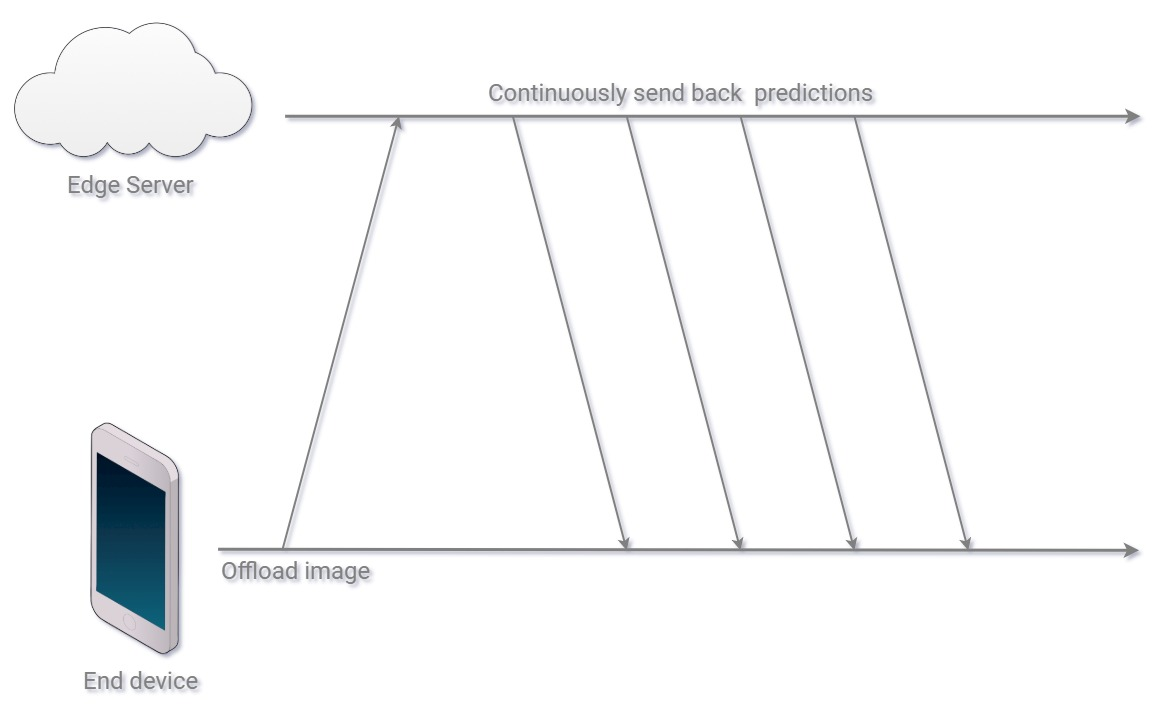
\includegraphics[width=\textwidth, left]{figures/models/timeline_all}
	
	

	\begin{minipage}[t]{.4\linewidth}
		\noindent
		{\large 
			\textsf{Supervisor: Qi Zhang} \\
			\textsf{Co-supervisor: Jianhui Liu}
			
		}
	\end{minipage}
	\begin{minipage}[t]{.59\linewidth}
	    \noindent
		% Logo could be included here
		
\includegraphics[width=100pt, right]{figures/logos/au}
		\vskip 1em
		
\includegraphics[width=100pt, right]{figures/logos/netx}
		\vskip 1em
		
\includegraphics[width=100pt, right]{figures/logos/stibo}
	\end{minipage}
    

    
    \textsf{Aarhus 2019}}
    \end{flushleft}
    \end{titlepage}
	\restoregeometry


    
    
	%\clearpage
	% Empty page after title page
	\begingroup
	\pagestyle{empty}
	\begin{center}
		\begin{LARGE}
			\thetitle \\
			\vskip 1em
			by\\
			\vskip 1em
			\theauthor
		\end{LARGE}
	\end{center}

	\vspace*{\fill}
	\begin{center}
		\begin{minipage}[t]{.5\linewidth}
			\centering
			
\includegraphics[width=\linewidth]{figures/logos/au}
			\hskip 1em
			
\includegraphics[width=.8\linewidth]{figures/logos/netx}
		\end{minipage}
		\vskip 3em
		\begin{minipage}[t][][b]{.3\linewidth}
			\textbf{\textsf{\theauthor}} \\
			Borggade 6k, 2., 8 \\
			8000 Aarhus C, Denmark \\
			Phone +45 2336 3745 \\
			alexkarlsen7@gmail.com \\
		\end{minipage}
		\hskip 10em
		\begin{minipage}[t][][b]{.3\linewidth}
			\textbf{Aarhus University} \\
			\textbf{Department of Engineering} \\
			Finlandsgade 22 \\
			5125 Edison \\
			8200 Aarhus N, Denmark \\
			Phone +45 8715 0000 \\
			eng@au.dk \\
			eng.au.dk \\
		\end{minipage}

	\end{center}
	\newpage
	\restoregeometry
	\setcounter{page}{1}
	
	\hypertarget{preface}{%
\chapter*{Preface}\label{sec:preface}}
 \blockquote{The master thesis have been accomplished at Department of Engineering at Aarhus University and facilitated by Stibo Accelerator. The work in fulfilment of the requirements for acquiring the degree of Master of Science in Computer Engineering. A special thanks is given to supervisor Qi Zhang, co-supervisor Jianhui Liu and the director of Stibo Accelerator Kim Svendsen.} \color{caption-color} 
 
 \vspace*{\fill}
 \begin{center}
 	 Aarhus, \today
 	 \vskip 10em
 	\begin{minipage}[c]{.5\linewidth}
		\hrulefill \\
 	\end{minipage}
 \end{center}


 
 \raggedleft\theauthor
\vskip 5em


	\endgroup
	\pagenumbering{Roman}
	\justify
	
	
	
    \hypertarget{abstract}{%
    \chapter*{Abstract}\label{sec:abstract}}
\begin{justify}
	\begin{small}
		{\textcolor{caption-color}{The thesis \textit{"\thetitle"}, investigates methods to reduce inference latency of deep neural networks (DNNs) for intelligent applications on the edge. This is important for emerging applications such as AR/VR, autonomous vehicles, mission-critical IoT applications, and others. These applications all require extremely low latency, which the conventional cloud intelligence approach cannot meet due to communication bottlenecks on the public internet. \newline
		The conventional, cloud-centric framework offloads sensor data, e.g., images from end devices to the central cloud in order to perform model inference and send the results back to the end devices. DNNs have been state-of-the-art for such tasks for the last decade and but only when run in large-scale data centers. However, as hardware for accelerated computing is becoming increasingly accessible, a new computing paradigm has emerged on the edge of the network.
		\newline Edge intelligence reduces communication latency by moving the processing of AI algorithms from the core of the network to the network edge using decentral servers and small scale data centers. Edge computing has many benefits such as lower communication latency, higher reliability and resilience, better security and privacy, scalability and context-awareness, and others. Despite being a fairly recent area of research, efforts have already been made in designing DNN models specially suited for edge computing by reducing the inference time. One of these is the early exit model. 
		\newline Early exiting models have been used to either reduce the mean inference time by allowing samples to exit the inference process at an early stage if a confident prediction can be obtained. We have implemented and trained early exiting models based on state-of-the-art DNN architectures and made a comprehensive evaluation of the promising accuracy-latency trade-off implied by early exiting. We have studied confidence threshold strategies for early exiting to reduce mean inference latency and improve reliability under delay constraints. 
		\newline
		Based on our findings, we propose a novel, flexible inference scheme, \acrfull{aee}, which can comply with more stringent latency requirements. The proposed scheme is implemented as a prototype using an Intel NUC as IoT end-device and NVIDIA Jetson TX2 and a GPU Workstation as edge servers and tested in a lab setup. The scheme takes advantage of the inherent properties of early exiting models. The end-device offloads image data to an edge server, which processes the DNN. While the DNN keeps running, the predictions via early exits will be sent back to the end device as soon as they are ready. The end-device might receive multiple predictions within the allowed time frame and can use information from all predictions to make a final decision. Our work reveals the new possibility to improve the reliability under stringent latency requirements, which cannot be fulfilled by conventional DNNs.
		}}
	\end{small}
\end{justify}
    
	\addcontentsline{toc}{chapter}{Abstract}
    \setglossarystyle{mcolindex}
    \printnoidxglossary[type=\acronymtype]%,numberedsection=autolabel]
    \addcontentsline{toc}{chapter}{Acronyms}
    
    
    \tableofcontents
    
    \pagenumbering{arabic}
    \setcounter{page}{1}
    
    
    \pagebreak

    
    
\hypertarget{introduction}{%
	\chapter{Introduction}\label{ch:introduction}}
%\thispagestyle{fancy}

Deep Neural Networks have in recent years outperformed traditional \gls{ml}, and achieved even super-human performance in \gls{cv} for image classification and object detection \cite{russakovsky_imagenet_2015}. Emerging applications, such as AR/VR, autonomous vehicles, mission critical IoT applications, could all benefit from \gls{ai} \cite{pettey_immersive_2018}. Opposed to traditional \gls{ml} algorithms, a \gls{dnn} requires tremendous computing power, which have made \gls{dnn}s infeasible for mobile and \gls{iot} devices. All these applications require extreme low latency of \gls{ai} decision feedback, which makes \gls{ci} infeasible \cite{zhou_edge_2019}. 

\acrlong{ei} reduces communication latency by moving the processing of AI algorithms away from cloud data centers at the core of the network, to the network edge using servers and small-scale data centers deployed in closer proximity to the application \cite{shi_edge_2016}. In chapter \ref{ch:edgeintelligence} we elaborate upon \gls{ei}. We describe the background of \gls{ei} and \gls{ei} inference architectures, and we present related work in reducing inference latency and cost of \gls{dnn}s deployed at the edge. Our main focus is early exiting models, due to the flexibility of reducing the inference latency by early exits using fewer layers of the \gls{dnn}. Methods to reduce inference latency at the edge are elaborated upon in \ref{sec:ei-fast-inference}. 

We investigate early exit \gls{dnn}s on image classification in chapter \ref{ch:earlyexit}. We describe early exits models, including the training and inference framework. We define an analytical model used for evaluation of the early exit and the conventional \gls{dnn}s. We implement the early exit models using the \gls{branchynet} framework \cite{teerapittayanon_branchynet:_2016} based on state-of-the-art \gls{resnet} \cite{he_deep_2015}, \gls{densenet} \cite{huang_densely_2016} models, and \gls{msdnet} \cite{huang_multi-scale_2017}, a model specifically designed for early exits. We contribute with a study of early exiting \gls{dnn}'s capability to trade accuracy for latency using different exit thresholds, and also early exiting for time-critical applications with deadlines.

In chapter \ref{ch:edgeoffloading}, we propose an inference scheme for time-critical applications named \acrfull{aee}. The scheme utilizes the flexibility of early exit models to produce increasingly confident predictions from deeper layers of the \gls{dnn} before the deadline. The scheme is applicable for both on-device inference and edge offloading. If \gls{aee} is deployed on the edge, the predictions are sent back to the device. Continuously sending back predictions is the best effort approach to cope with latency uncertainties from both computation and communication. \gls{aee} suffers less from sporadic, unexpected delays. Upfront optimal exit decision, as proposed in \cite{li_edge_2018}, do not account for these uncertainties. Due to the limited delay overhead from additional classifiers we argue, that our approach is able to reach the same exit, as in \cite{li_edge_2018}. We show that \gls{aee} has the potential to enable services with stringent latency requirements, which cannot be realized by the conventional DNNs. We implement \gls{aee} and setup experiments on an Intel NUC and a Jetson TX2. We present our results and show that the solution improves service reliability under stringent delay requirements compared to on-device inference.

In chapter \ref{ch:conclusion} we conclude upon the thesis.

    \section{Related work}

Read cascade neural net for inspiration to this introduction

Over the last couple of years an increasing interest in reducing the inference time of intelligent applications to be able to run on less powerful mobile and \gls{iot} device in real-time applications. The survey \citetitle{zhou_edge_2019} by \citet{zhou_edge_2019} review the current state within the research field of \gls{ei}. The survey includes training and inference of \gls{dnn} on the edge and categorizes similar approaches to improve training \gls{ei} application and services and proposals to shorten the inference time in such setups. This thesis is mainly concerned with reducing inference time.

\section{Our contribution}

We look at combining early exiting with model partitioning. 

The objective of this thesis is, taking mobile AR applications as use case, to design and implement of MEC offloading deep learning algorithms to maximize the inference reliability while meeting the service latency deadline. The thesis will design feasible offloading schemes, such as deep neural network partitioning, preprosssing (feature extractions), in objective detection and classification. The proposed schemes will be implemented using Raspberry Pi and Jetson TX2. The communication and computation latency, as well as the inference accuracy and reliability will be measured and analyzed.
    \chapter{Theory}

\section{\gls{mec}}

Mobile computing, \gls{mcc}, \gls{iot} \gls{ei}

\section{\gls{ai}}

\gls{ml}, supervised learning

\gls{cv}, recognition, localization, detection, segmentation

\gls{dl}, training, inference, convolution layers, weights, transfer learning 



    \hypertarget{earlyexiting}{%
	\chapter{Early Exiting}\label{ch:earlyexit}}
\thispagestyle{fancy}

In this chapter we study accuracy latency trade-off of the early exiting \gls{dnn}s, by experimentation of exit thresholds and delay thresholds. We have found, that the early exiting have capabilities to better accommodate delay threshold, than conventional single-exit \gls{dnn}s. The chapter is structured as follows, in section\ref{sec:ee-branchy-vs-cascaded}   present the early exit proposals \gls{branchynet} ann Cascaded \gls{dnn}. In section \ref{sec:ee-metrics} we define the metrics used in our experiments. In section \ref{sec:ee-exp-setup} we descibe our experimental setup. In Section \ref{sec:ee-implementation} we describe the implementation details of our early exiting models B-\gls{resnet} and B-\gls{densenet}. In section \ref{sec:ee-results} we present our results of training the models and experimenting with the fast inference framework using exit threshold and delay threshold. In section \ref{sec:ee-summary} we discuss our results.

%Early exiting \gls{dnn} draws inspiration from another \gls{cv} algorithm, Viola-Jones \cite{viola_rapid_2001}. Viola Jones Face Detection was proposed in \citeyear{viola_rapid_2001}. The idea is a stacking or cascaded less accurate predictors to build a strong predictor. The predictors increasingly gain confidence when running the algorithm which termintates when the confidence has reached a threshold. Early exiting \gls{dnn} likewise stacks multiple classifiers. The \gls{dnn} can too be terminated, when a prediction with satisfying confidence is obtained. 



% and have primarily been used to solve two challenges in current literature.
%
%\begin{enumerate}
%	\item Reducing average inference latency and power consumption by letting samples prematurely exit the model based on a threshold measure of confidence \cite{teerapittayanon_branchynet:_2016}.
%	\item Comply with application time constraints by exit selection or sub-model selection. By only inference samples up to a selected exit possible to meet stringent delay constraints and reduce waste of computation \cite{li_edge_2018}. 
%\end{enumerate}

\section{BranchyNet vs. Cascaded DNN} \label{sec:ee-branchy-vs-cascaded}

\gls{branchynet} \cite{teerapittayanon_branchynet:_2016} and cascaded \gls{dnn} \cite{leroux_resource-constrained_2015} was published around the same time. We describe the two very similar proposals and how they differ.  Cascaded \gls{dnn} adds intermediate classifiers after a layer, or a block of layers in a \gls{dnn}, wheres \gls{branchynet} constructs early exit branches with additional layers, see figure \ref{fig:cascaded-vs-branchy}.

\begin{figure}
	\centering
	\subfloat[Branchy AlexNet, Source \citetitle{teerapittayanon_branchynet:_2016} \cite{teerapittayanon_branchynet:_2016}]{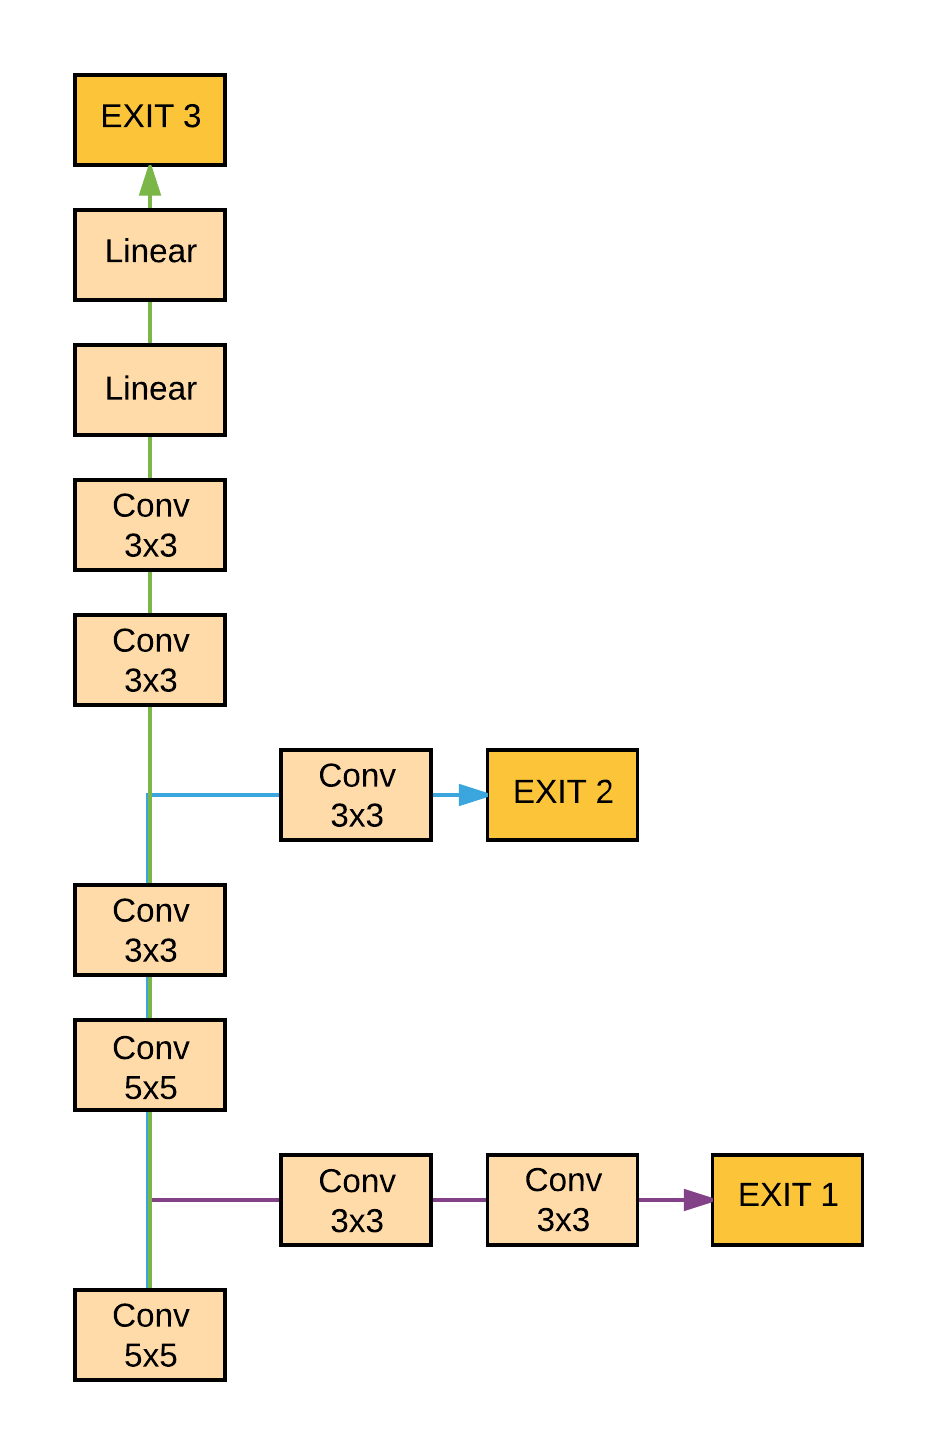
\includegraphics[height=.3\textheight]{figures/articles/branchynet}}
	\hspace{2em}
	\subfloat[Cascaded \gls{dnn}, Source \citetitle{leroux_resource-constrained_2015}\cite{leroux_resource-constrained_2015}]{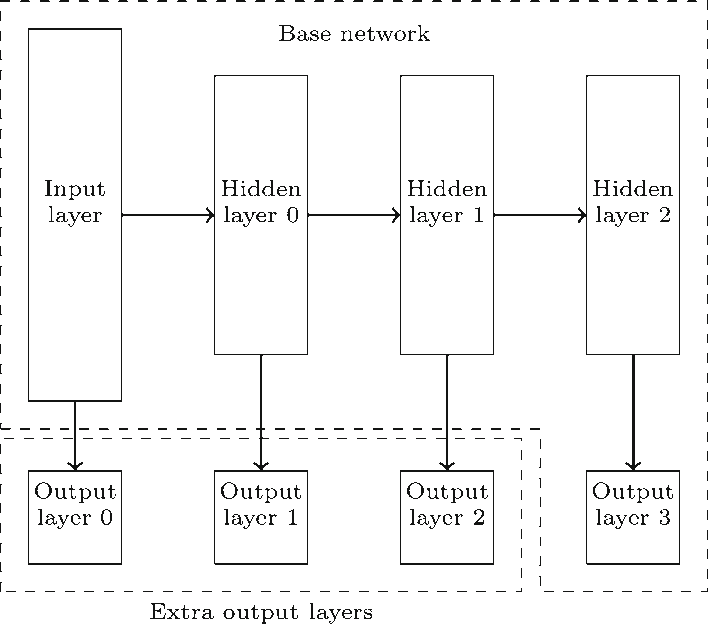
\includegraphics[height=.3\textheight]{figures/articles/cascade_dnn}}
	\caption[\gls{branchynet} vs. Cascaded \gls{dnn}]{\gls{branchynet} vs. Cascaded \gls{dnn}}
	\label{fig:cascaded-vs-branchy}
\end{figure}

Early exiting relies on the assumption, that the majority of samples are easy to classify correctly, and that \gls{dnn}s only have become deeper to accurately classify more difficult samples. As figures \ref{fig:hardvseasydog} exemplifies, samples where the object is easily separated from the background, are not occluded, and are viewed from angles which makes it easier to classify. Contrary samples that are not, are harder, additionally if the sample, should be discriminated from classes, with similar features are difficult such as different dog breeds etc. These examples have been found by running an early exit model. The hard examples have been found from looking at samples, that the \gls{dnn}s failed to classify, or can only classify using the last exit. The easy example are found by looking at samples, that can be correctly classified with high confidence by the first exit. 

\begin{figure}
	\captionsetup[subfigure]{justification=centering}
	\centering
	\subfloat[bluetick]{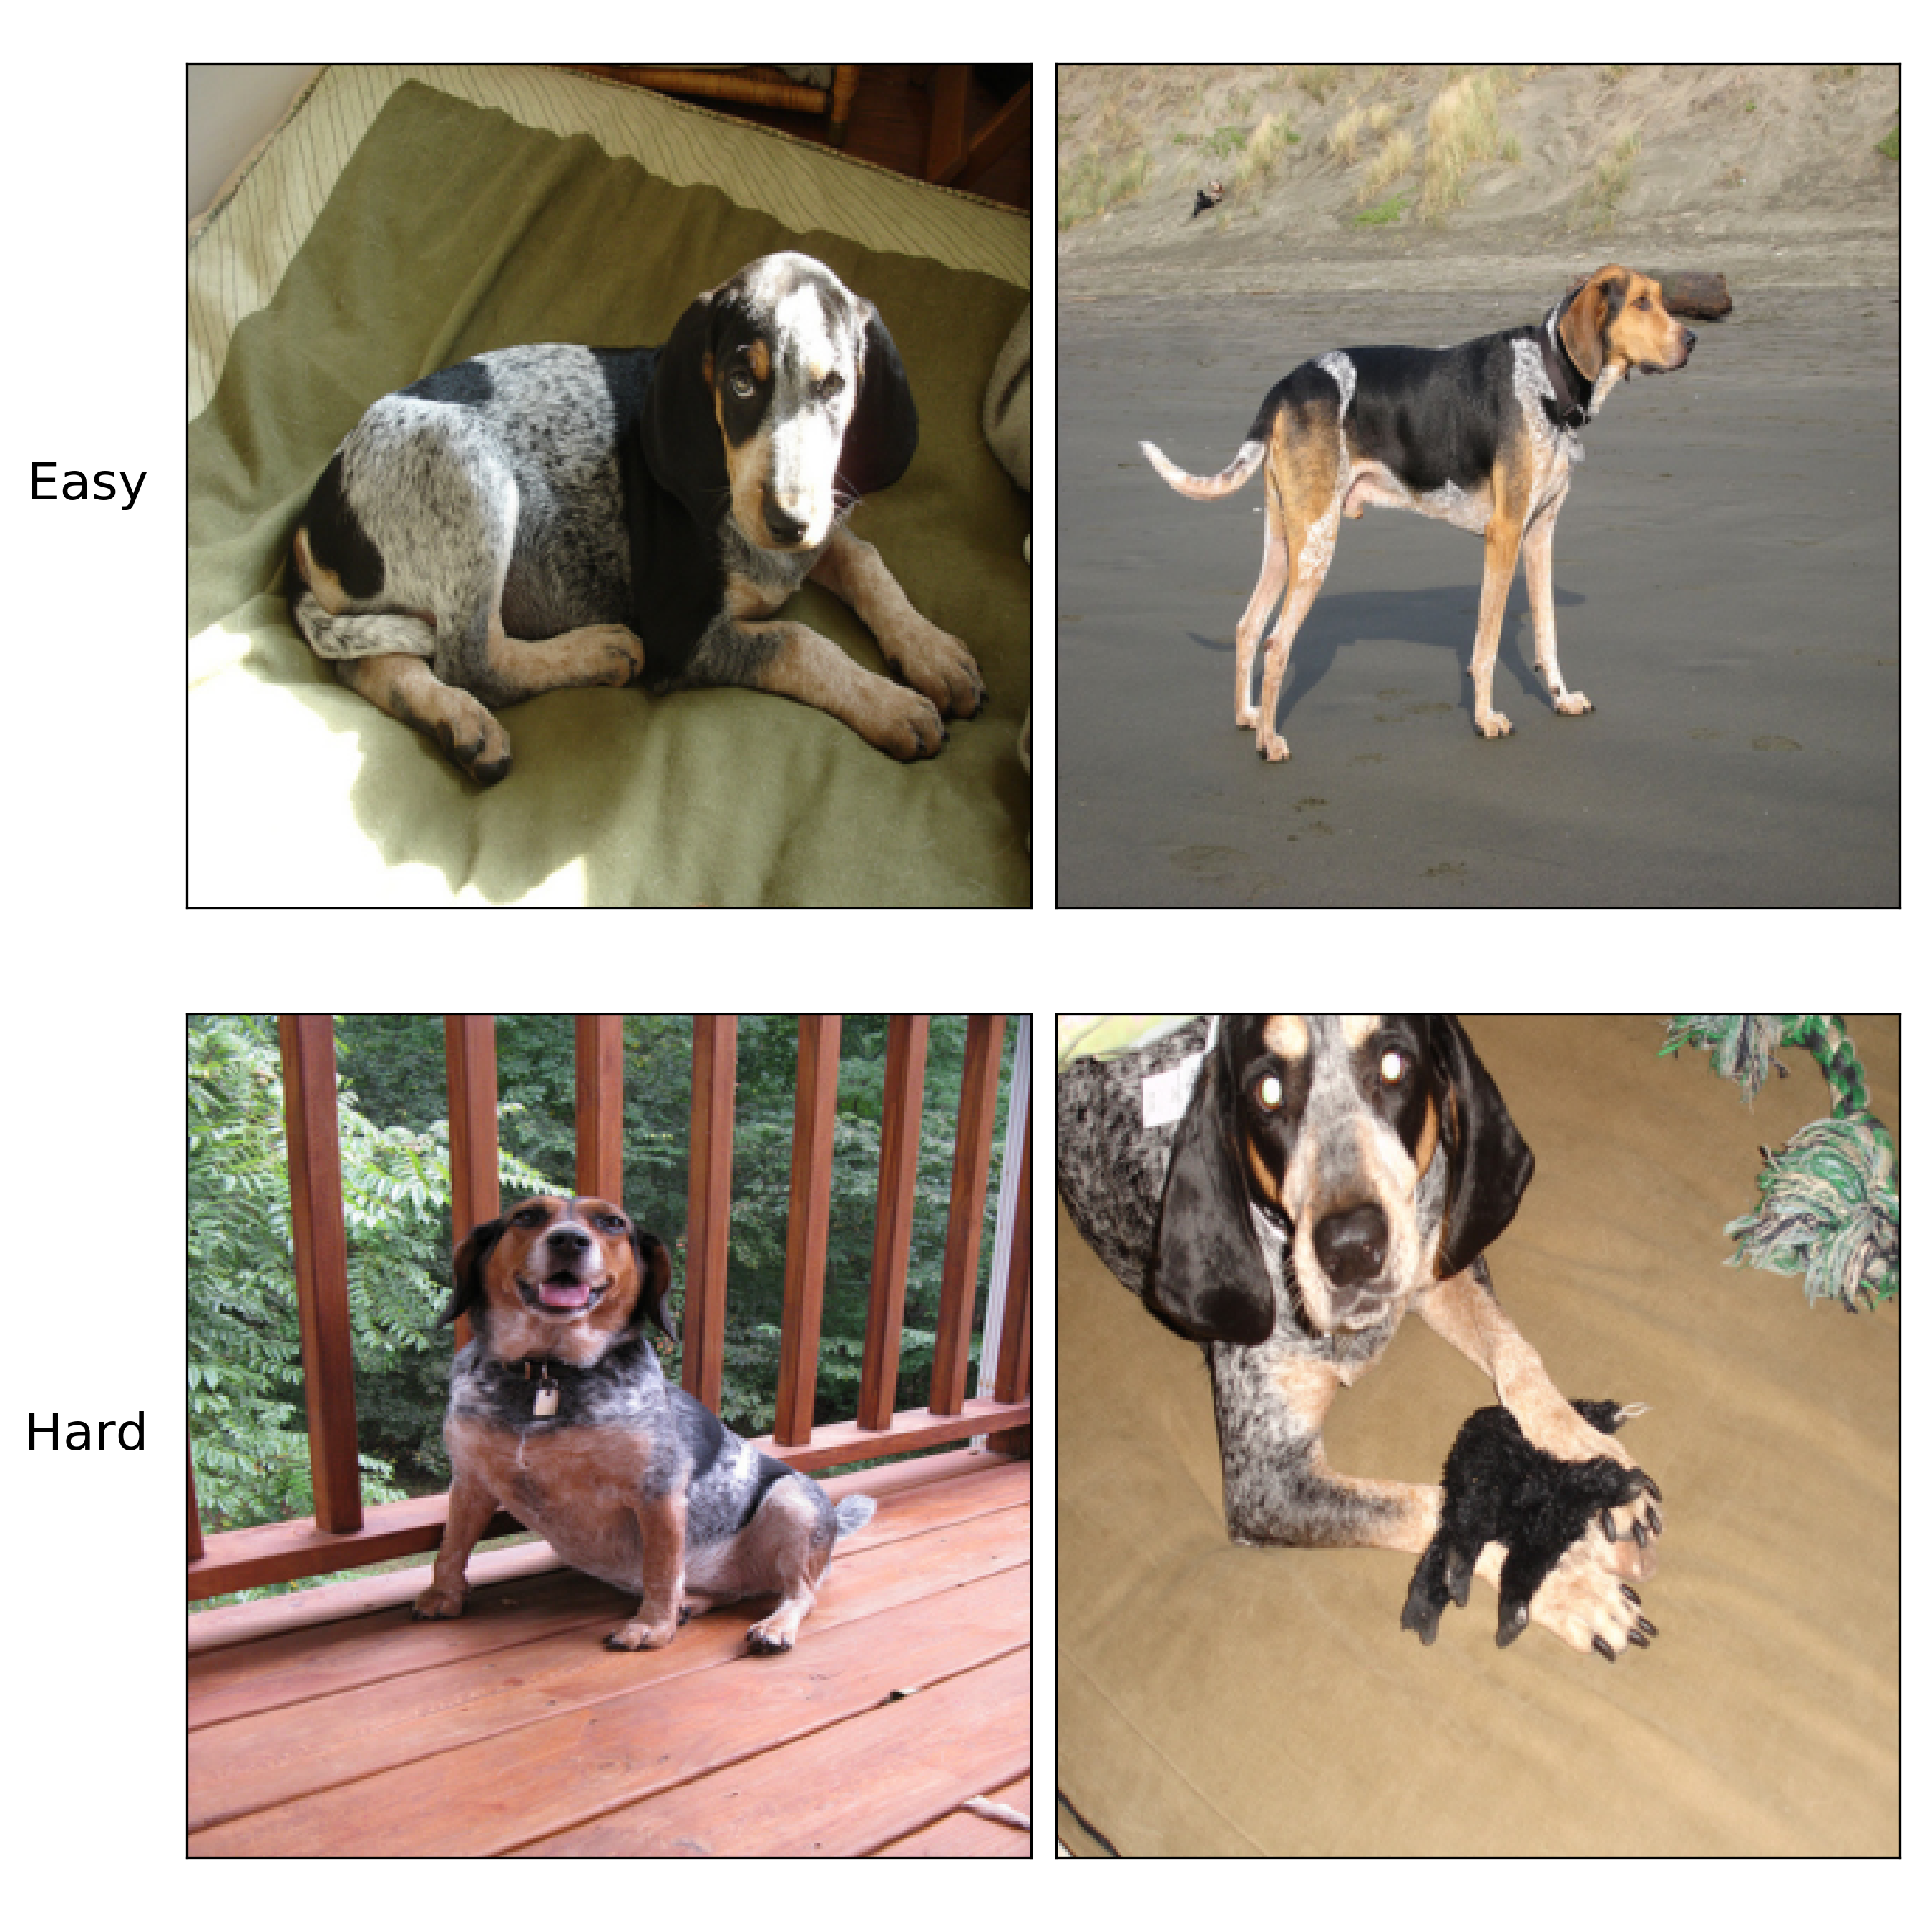
\includegraphics[width=0.5\linewidth]{figures/illustrations/hard_vs_easy_dog}}
	\subfloat[flamingo]{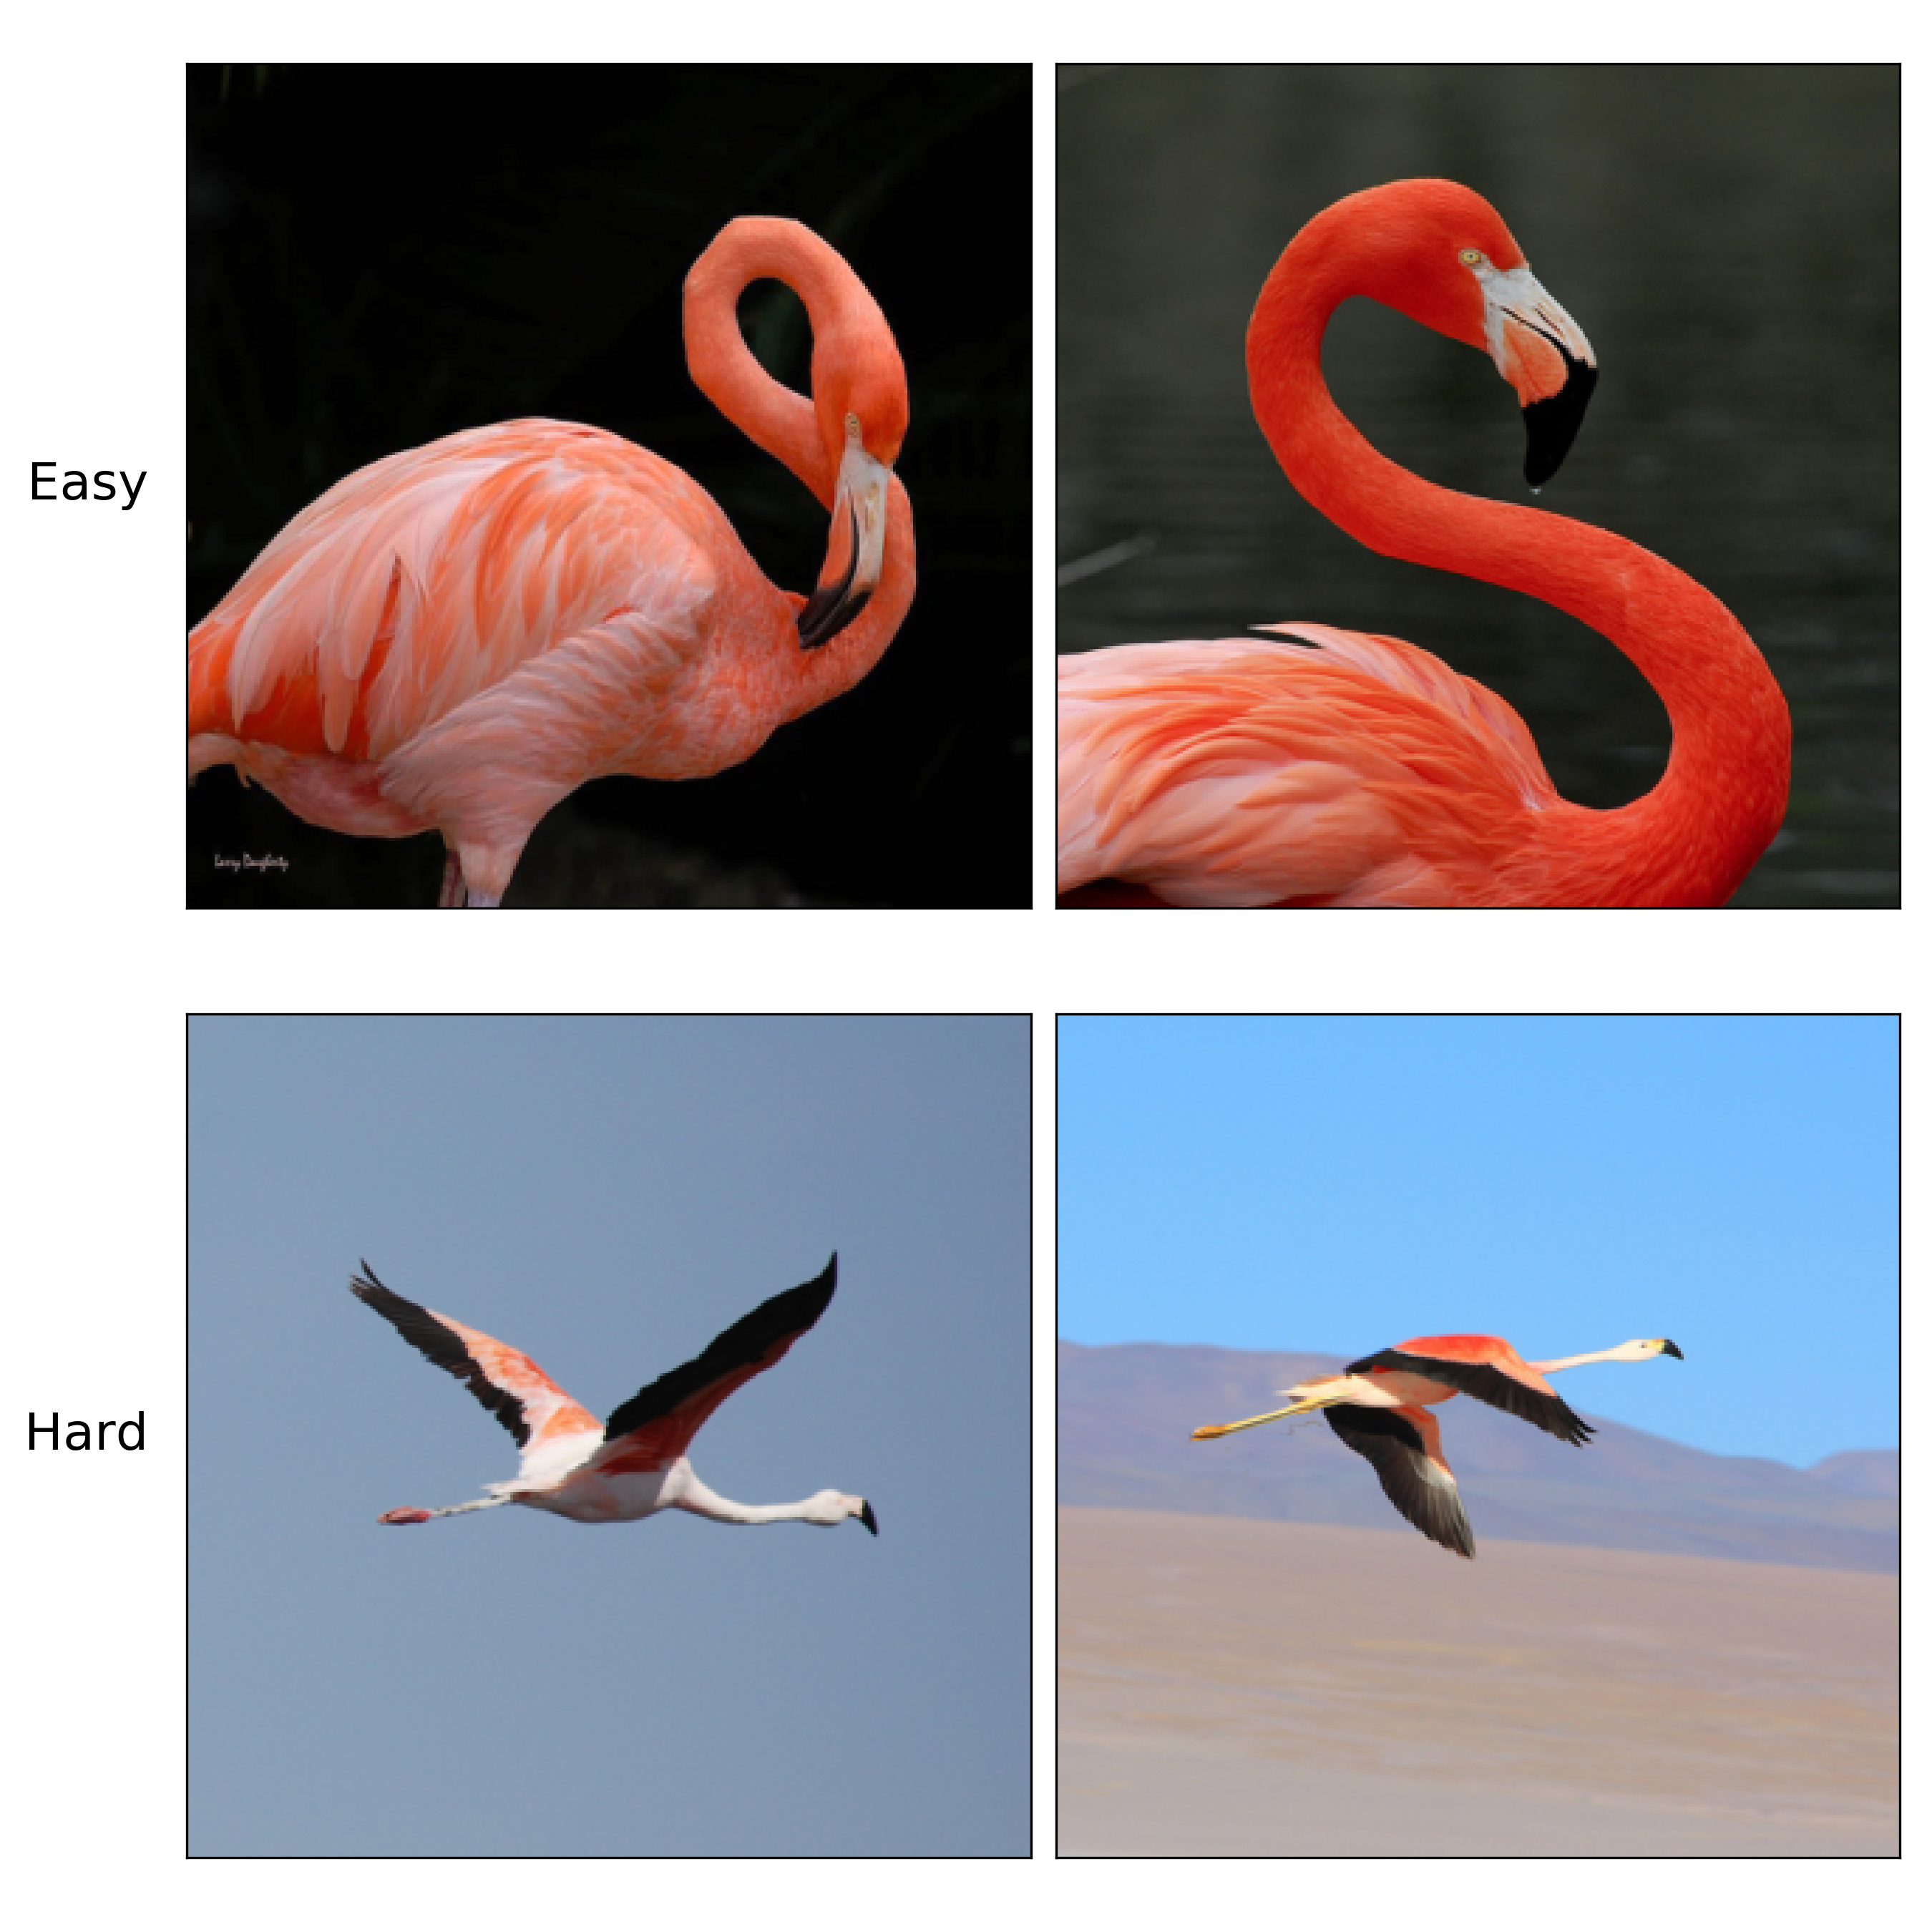
\includegraphics[width=0.5\linewidth]{figures/illustrations/hard_vs_easy_flamingo}}
	\caption[Easy vs. Hard Samples]{Easy vs. Hard Samples}
	\label{fig:hardvseasydog}
\end{figure}

\paragraph{Fast Inference Framework} The inference framework for the two proposal \gls{branchynet} and Cascaded \gls{dnn} are almost identical. A sample is inferred up to an exit and based on an exit criteria, it is decided to exit or to continue the inference. The only difference is the choice of exit threshold. Cascaded \gls{dnn} uses the softmax score of the prediction, and evaluates if the score higher than a selected threshold, it is exited. \gls{branchynet} determines the entropy of the softmax output, and evaluates if the entropy is less than a selected threshold, the sample is is is exited.

The algorithm we use for early exit fast inference is provided in listing \ref{lst:score-margin-inference}. Note the algorithm uses the confidence threshold for exit decision.

\begin{minipage}{\linewidth}
	\begin{lstlisting}[language = {}, mathescape=true, caption={Early Exit using Score-margin }, label={lst:score-margin-inference}]
procedure $\textsc{EarlyExitFastInference}$$(x, T )$
	for $k = 1\dots K$ do
		$z = f_{exit_k}(x)$
		$ \hat{y} = softmax(z) $
		if $\hat{y} > T_k$ then
			return $\arg \max \hat{y}$
	return $\arg \max \hat{y}$ 
	\end{lstlisting}
\end{minipage}

Early exiting have shown promising result in other works. In \cite{berestizshevsky_sacrificing_2019}, they suggest removing convolutional layers of branches in \gls{branchynet}, to reduce the amount of branch computation. They show a 2 $ \times $ speed-up at only the cost of 1 \% accuracy using two fully-connected layers in exits.

In \cite{kaya_shallow-deep_nodate}, \emph{Overthinking}, the phenomena where an early exit correctly classifies an input, but a later exit makes it wrong is investigated. They propose to use the highest scoring prediction from all exits to cope with overthinking. 

\paragraph{Training Framework} 
Training cascaded \gls{dnn}, in \cite{leroux_resource-constrained_2015} it is proposed to train a network using a single end-classifier. Once the model has reaches convergence, the intermediate classfiers are attached and the entire network is trained for one single epoch, before freezing the network weights and training the classifiers. This is equivalent to use a pre-trained model and convert it to a cascaded model. The approach was tested and gave unsatisfactory results, see figure \ref{fig:frozen-b-resnet-miniimagenet-100}. In \cite{leroux_cascading_2017}, the follow-up paper to cascaded \gls{dnn}, they too train a frozen base network on the ImageNet dataset, but does not achieve better performance for early exit classifiers.  

The \gls{branchynet} approach is remarkably similar. In \cite{teerapittayanon_branchynet:_2016} they define the \gls{branchynet} loss function, as an extension of the widely used softmax cross-entropy loss function.
\begin{align}
L\left(\mathbf{y},\hat{\mathbf{y}}\right) = - \frac{1}{C} \sum_{j =1}^{C} y_c \log \hat{y}_c
\end{align}
Where $ \bm{y} $ is a on-hot encoded ground truth vector, $ \bm{\hat{y}} $ is the output score vector of the softmax classfier and $ C $ is the number of classes and $ c \in \left[1, C\right] $ is the class labels. The softmax function is defined as
\begin{align}
 \bm{\hat{y}} = \frac{e^{z}}{\sum_{j=1}^{C}e^{z_c}}
\end{align}
where $ z $ is the output of the \gls{dnn}.
	
The \gls{branchynet} loss function is defined as the weighted sum of the softmax cross-entropy loss of each branch-prediction. 
\begin{align}
	L_{\mathrm{BranchyNet}}(\hat{\mathbf{y}},\mathbf{y};\theta) = \sum_{n=1}^{N} w_n L \left(\hat{\mathbf{y}}_{n},\mathbf{y};\theta\right)
\end{align}
Where $ \bm{\hat{y}} $ is the output score vector of exit $ n $, $ w_n $ is the weight for exit $ n $ and $ \theta $ represents the parameters of the layers from an entry point to the exit point $ n $.

They claim, that the joint-optimization of multiple exits provides a regularization effect, thus countering over-fitting and potentially improves test accuracy. Additionally is also mitigates vanishing gradient, due to additional gradient signal from the early exits, which promotes more discriminative feature in early layers. In \gls{googlenet} \cite{szegedy_going_2015} auxiliary classifiers are too place in the middle of the network to counter vanishing gradients. However, that is also the only purpose of the auxiliary classifiers, as they are only used when training the network. Thus, no samples can exit the inference process prematurely. 

In \gls{branchynet}, they have also too found, that first training the network end-to-end or using a pre-trained model, and then attach the intermediate exits/classifiers both improves the performance and shortens the training time, as in cascaded \gls{dnn}. However, they do not suggest to freeze the features of the base model, but to train the entire model. We have tried both freezing and unfreezing the network base and have found, that training the entire model is the far superior approach, see figure \ref{fig:b-resnet-miniimagenet-100}. 

In the next section we explain the \gls{msdnet} \cite{huang_multi-scale_2017}, a novel \gls{dnn} specifically designed for early exits.

\section{Multi-Scale Dense Network}

A study in \cite{huang_densely_2016} show that densely connected layers of \gls{densenet} are more suitable for early exiting, than the popular \gls{resnet} architecture build of residual blocks. Densely connected block uses a concatenation of features from all layers for final classification. The combination of  general feature and increasingly more specific and complex features are shown to be important for early exiting models. This finding have been used to come of the novel \gls{dnn} design. A further elaboration of the network layers are found in section \ref{sec:ee-implementation}. Figure \ref{fig:msdnet} from the original article Multi-scale path on the vertical axis and the depth on the horizontal axis. The figure show the stacking of filters that are concatenated (c) along both axes. Each block contain an exit with a classifier.

\begin{figure}
	\centering
	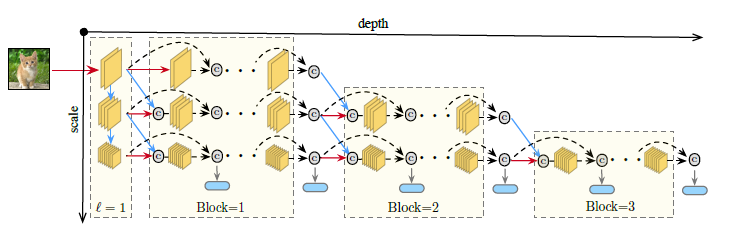
\includegraphics[width=\linewidth]{figures/models/msdnet}
	\caption[\gls{msdnet} Architecture]{\gls{msdnet} Architecture, Source: \citetitle{huang_multi-scale_2017} \cite{huang_multi-scale_2017}}
	\label{fig:msdnet}
\end{figure}

The work addresses two main problems concerning early exiting. The first problem is the lack of coarse-level features in early classifiers. Traditional \gls{dnn}s uses stacking of layers to get coarse level features, which the early classifier lacks, thus giving unsatisfactory high error-rates. Multi-scale feature maps addresses this issues by preserving high-resolution information and allow constructing coarse-level features for all classifiers in the network.

The second problem is early classifiers interfere with later classifiers. The early classifiers might cause early features to be optimized for the short-term by collapsing information prematurely, thus harming the later and final classifiers. Their study reveals, that densely connected layers suffers much less from intermediate classifiers than residual layers, as a layer is connected to all previous layer and is therefore able to recover collapsed information. We elaborate upon the two different types of layers in section \ref{sec:ee-implementation}. We experiment with \gls{resnet}, \gls{densenet} and \gls{msdnet} in our experiments.

In the next section we describe the mathematical models used to evaluate the latency, accuracy and early exiting capabilities using confidence and delay thresholds.

\section{Analytical Model} \label{sec:ee-metrics}

In this section we define the analytical model used for our experiments. We compare conventional models with early exiting models. Most \gls{dnn}s are build of blocks of convolution and pooling layers, or at least the ones we use, and exits i.e. classifiers. We adapt the same notation for the early exiting inference model and the conventional inference model with a single exit at the end of the \gls{dnn}, see figure \ref{fig:inference_models}.
	\begin{figure}
		\centering
		\captionsetup[subfigure]{justification=centering, farskip=1pt,captionskip=1pt}
		\subfloat[Conventional Inference Model]{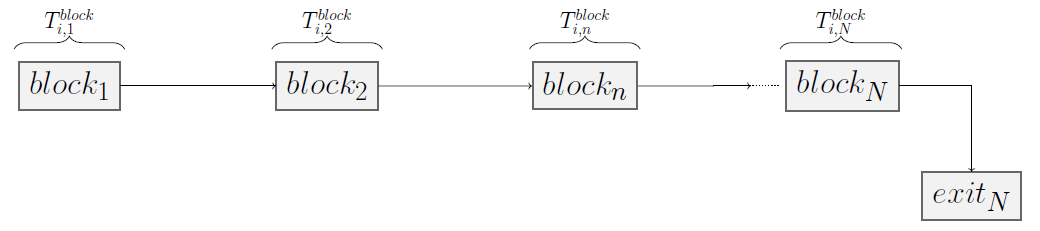
\includegraphics[width=.7\linewidth]{figures/models/conv_math}}
		\hfill
		\subfloat[Early Exit Inference Model]{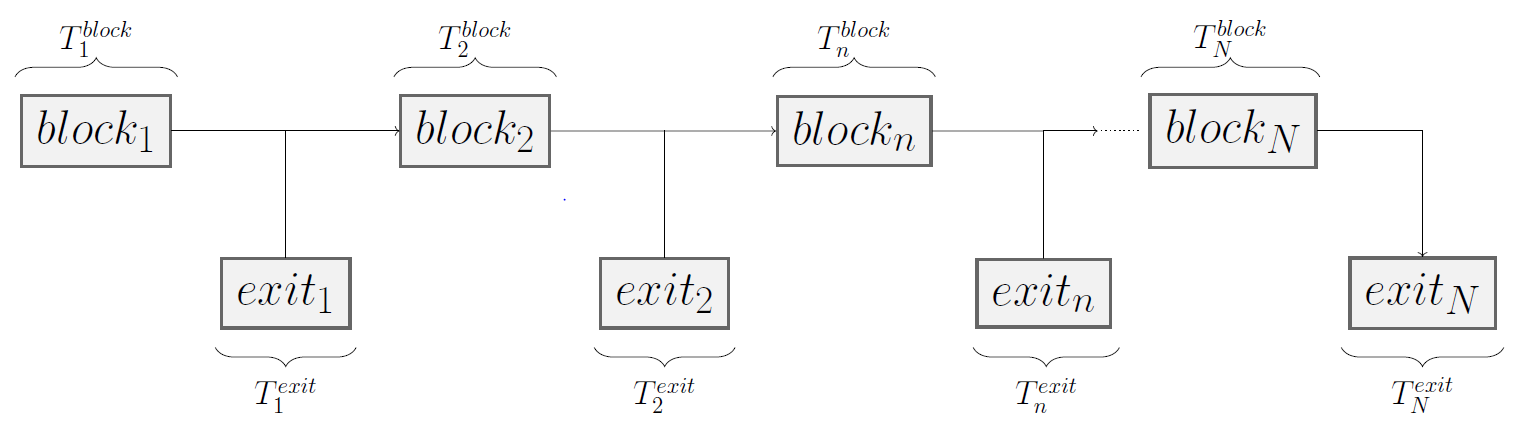
\includegraphics[width=.7\linewidth]{figures/models/exit_math}}
		\caption[\gls{dnn} structure]{\gls{dnn} inference models: A \gls{dnn} is constructed by stacking layers of non-linear function on top of each other to form a \gls{dag}. The layers are typically grouped into blocks, and a classification layer is attached at the end of the network, i.e. exits in our models.}
		\label{fig:inference_models}
	\end{figure}	
	We define the inference latency for both models, classification accuracy, early exit condition and our problem formulation. Assume $ C $ denotes the number of image classes, $ N $ denotes the number of the exit points in a DNN, $ I $ denotes the number of images.

	\begin{enumdescript}
		\item[Inference Latency] is defined as the response time for a \gls{dnn} to provide a prediction i.e. the time from input to output. 

		Assume:
		\begin{itemize}
			\item $T_{i,n}^{block}$ denotes the runtime inference an image $ i $ to the $ n $th block of the \gls{dnn} $ i $ for $ \left(1\leq n \leq N, 1 \leq i \leq I\right) $
			\item $T_{i,n}^{exit}$ denotes the runtime of the exit $ n $  to process image $i$ for $ \left(1\leq n \leq N, 1 \leq i \leq I\right) $
		\end{itemize}
		\begin{enumdescript}
			\item[Inference Latency Conventional Model] The conventional inference model only have a single exit at block $ N $, hence all $ N $ blocks of the \gls{dnn} must have inferred the image $ i $ before a classifications is reached at exit $ N $. Thus the latency model for a conventional inference model is presented as
			\begin{align}
			T^{ci}_{i}= \sum_{j=1}^{N} T_{i,n}^{block} + T_{i,N}^{exit}
			\end{align}
			\item[Inference Latency Early Exit Model] The early exit inference model is adaptive. The inference of image $ i $ can terminate at any exit $ n $. If the classification exits from exit point $ n $, then the latency model for early exit inference model is presented as
			\begin{align}
			T_{i,n}^{ee}=\sum_{j=1}^{n} \left(T_{i,n}^{block} + T_{i,n}^{exit} \right) 
			\end{align}
			The additional classifiers of the early exit inference model add a overhead compared to the conventional inference model, however it may not be required to run all $ n $ blocks and classifiers of the early exiting inference model. 
		\end{enumdescript}
		
		\item[Classification Accuracy] is the defined as the fraction of correctly classified samples out of all inferred samples. The inference accuracy of exit point $ n $ can be expressed by
		\begin{align}
		\bar{A}_{n}=1-\frac{1}{I} \sum_{i=1}^{I} \mathbb{I}\left(\left|\hat{c}^*_{i,n}-c_{i}\right|\right) \label{eq:accuracy}
		\end{align}
		%We can express the ground truth as a one-hot encoded vector $ \bm{y}_i $
		where the ground truth class label of image $ i $ is $ c_i \in \left[1, C \right] $.
		
		an $ \mathbb{I(\cdot)}  $ is a indicating function defined by
		\begin{align}
		\mathbb{I}(a)= \begin{cases}
		0, & \mathrm{if\:} a \leq 0, \\
		1, & \mathrm{otherwise}
		\end{cases}
		\end{align}
		    		
		Note for the conventional model only $ A_N $ can be expressed, as the model only has a single exit.
		
		The prediction output from the softmax classifier is denoted
		\begin{align}
			\mathbf{\hat{y}}_{i,n} = \left[\begin{array}{ccccc}\hat{y}_{i,n,1} & \hat{y}_{i,n,2} & \hat{y}_{i,n,c} & \dots & \hat{y}_{i,n,C}\end{array}\right]
		\end{align}
		Where $ \hat{y}_{i,n,c} $ denotes the score of class $ c $ from exit point $ n $ by processing image $ i $
		
		The prediction is the highest scoring class of the softmax output. The class label of the prediction is denoted $ \hat{c}^*_{i,n} $ and is expressed as
		\begin{align}
		\hat{c}^*_{i,n} = \arg \underset{c}{\max}\: \mathbf{\hat{y}}_{i,n}
		\end{align}
		The score associated the class label is of image $ i $ from the exit point $ n $ is
		\begin{align}
		\hat{y}^*_{i,n} = \underset{c}{\max}\: \mathbf{\hat{y}}_{i,n}
		\end{align}
	
		Note that the prediction to go through the entire \gls{dnn} is $ \bm{\hat{c}}^*_i  = \arg \underset{c}{\max} \bm{\hat{y}}_{i,N} $, i.e. the last exit $ N $ of the early exit model, or equivalent to the prediction of conventional inference model.
  
		\item[Early Exit Condition] we define the early exit condition based on the output of our scoring function $ f_\phi(\bm{\hat{y}}_{i,n}) $, given the score vector $ \bm{\hat{y}}_{i,n} $ for image $ i $ at exit point $ n $. An image $ i $ is allowed to exit the model at exit point $ n $, if a score threshold $ \gamma $ is surpassed. 
		
		We assume $	\gamma \in \left[0,1\right] $, as the all scores of  $ \bm{\hat{y}}_{i,n} $ sum to 1. Note that, although the score threshold could be different for each exit point, in our experiments, we use the same threshold, since we are concerned with the latency. Selecting a higher threshold value at an early exit, will cause less samples to exit and promote use of later exits, which will cause additional inference delay. It is seen in \cite{teerapittayanon_finding_2018}, that finding different threshold values for the exits can improve the accuracy.
		
		We express the probability of early exit at exit $ n $, given the score function. 
		\begin{align}
		\overline{F}^{exit}_n = \frac{1}{I}\sum_{i=1}^{I} \mathbb{I} \left(\gamma-f_{\phi}\left(\bm{\hat{y}}_{i,n}\right) \right)
		\end{align}
		Where $ f_\phi\left(\bm{\hat{y}}_{i,n}\right) $ is a scoring function and for notation simplicity we write 
		\begin{align}
			f_{\phi}\left(\bm{\hat{y}}_{i,n}\right) = \begin{cases}
			 	f_{max}\left(\bm{\hat{y}}_{i,n}\right)\\
			 	f_{margin}\left(\bm{\hat{y}}_{i,n}\right)
			\end{cases}
		\end{align}
		which means we can choose to use either one. Next We define two different score functions.
		
		\begin{enumdescript}
			\item[Score-Max] the score-max function $ f_{max}(\cdot)$ also used in \cite{leroux_resource-constrained_2015}, is a simple function, that takes the score vector $ \bm{\hat{y}}_{i,n} $ of image $ i $ at exit $ n $ as input and outputs the maximum value of the vector. We express it as 
			\begin{align}
			f_{max}\left(\bm{\hat{y}}_{i,n}\right) = \underset{c}{\max} \bm{\hat{y}}_{i,n}
			\end{align}
			\item[Score-Margin] the score-margin function $ f_{margin}(\cdot)$, is defined and used in \cite{park_big/little_2015}. The function also takes the $ \bm{\hat{y}}_{i,n} $ as input and returns the difference between the two largest elements. We express it as
			\begin{align}
			f_{margin}\left(\bm{\hat{y}}_{i,n}\right) = \hat{y}_{i,n}^{1st} - \hat{y}_{i,n}^{2nd}
			\end{align}
			where $ \hat{y}_{i,k}^{1st} $ denotes the largest element of $ \bm{\hat{y}}_{i,n} $ 
			and $ \hat{y}_{i,n}^{2nd} $ the second largest element of $ \bm{\hat{y}}_{i,n} $.
			
		\end{enumdescript}
	
	\item[Reliability] our main concern is time-critical application. We define the reliability as the fraction of samples, that con be correctly classified given a latency threshold $ \delta $.
	
	\begin{align}
	R= \bar{A} \cdot (1-\overline{F}^{to})
	\end{align}
	
	The timeout probability $ \overline{F}^{to} $ is defined as the number of samples not able to meet the delay requirement out of all samples in the set.
	\begin{align}
	\overline{F}^{to}=\frac{1}{I}\sum_{i=1}^{I} \mathbb{I}\left(T_{i}^{cmp}-\delta\right)
	\end{align}
	Where $ T_{i}^{cmp} $ denotes computation time irregardless of conventional inference model with a single exit, or early exit models with multiple. We only have a delay violation if $ T_i^{cmp} \leq \delta $, i.e. the model have not provided a single prediction within the time frame. Thus, if no exit of the model can meet the delay requirements and a prediction cannot be acquired, it is treated as a misclassification. 
		
	\item[Problem formulation] we select exit point for each image and optimize its accuracy with a latency constraint. The inference time of image $ i $ at exit $ n $, cannot be greater than or equal to our latency threshold $ \delta $. 
	
	\begin{maxi}
		{n}{\bar{A}_{n}}
		{}{}
		\addConstraint{T_{i,n}}{\leq \delta}
	\end{maxi}
%	where $\vec{n} = \left[n_1,,n_2, \dots, n_I\right]$. 
	
	To solve this problem, instead of making decision before processing the image, we simply use the best effort way, i.e., feed each exit results back and let user decide the prediction. For three reasons:
	\begin{enumerate}
		\item latency uncertainty make it hard to make decision in advance
		\item algorithm to make decision may take time
		\item going through classifier of each exit point would not take too long time.
	\end{enumerate}
		
	\end{enumdescript}


In the next section we describe our implementation of early exit models.

\section{Implementation} \label{sec:ee-implementation}

In this section we describe our implementation of early exit models. We have implemented \gls{bresnet} and \gls{bdensenet}.  

\subsection{Branchy-ResNet} 

In this section is the residual layer, the building block of the residual network explained. Followed by a design description of \gls{bresnet}.

The depth of \gls{dnn}s is of paramount importance to extract increasingly richer features from images to obtain highly accurate classification models. Training very deep models with more than ten layer for convergence is not easy due to vanishing/exploding gradients. Residual Networks or \gls{resnet} \cite{he_deep_2015} have for long been a state-of-the-art network and won ILSVRC15 using 152 layers. The network is build of residual blocks, a \gls{dnn} layer designed for extremely deep networks. 

Just as plain \gls{vgg} networks \cite{simonyan_very_2015}, residual networks is still a stacking of convolutional layers. The \gls{resnet}, however, adds a shortcut connection, which skips a layer or a block of layers. The skip connection adds the identity of input to the output of the layers/block, see figure \ref{fig:residualblock}

\begin{figure}
	\centering
	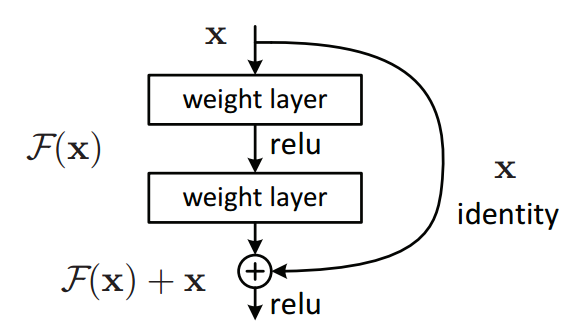
\includegraphics[width=.5\linewidth]{figures/models/residualblock}
	\caption[Residual Block]{Residaul Block}
	\label{fig:residualblock}
\end{figure}

Information from earlier layers are preserved by the residual, which diminishes the vanishing gradient problem. Thus this type of network have shown to be easier to train compared to it’s plain counterpart and able to obtain far superior accuracy.  

Very deep residual networks comprised of up to 152 layers have also shown to be far more efficient requiring less \gls{flop}s, than \gls{vgg}16 comprised of only 16 layers, by introducing a bottleneck unit. The bottleneck reduces the dimensions, applies the concolutional filters, and then restores the dimensions.

The residual networks proposed in \cite{he_deep_2015} are grouped into 4 resolutions block each of which downsamples the input data. The network are proposed with different number of layers (18, 34, 50, 101, 152) exemplifying th ability to train extremely deep networks. Table \ref{tbl:resnet101} describes the blocks and layers of the \gls{resnet} architecture. \gls{pytorch} provide implementations of these networks. The implementations can be trained from scratch or can be initialized with downloadable pretrained weights based on ImageNet. \gls{resnet}101 have been chosen for this project, as it has comparable depth to the smallest available \gls{pytorch} \gls{densenet}-121 implementation and also have similar inference latency on a Titan Xp (8.90ms and 8.93ms) \cite{bianco_benchmark_2018}.

\small
\begin{center}

\begin{minipage}[c]{\linewidth}
\begin{longtabu}{>{\bfseries}X|X[c]|X[2c]}
	\caption[\gls{resnet}101 description]{\gls{resnet}101 description. The table describes the blocks of \gls{resnet}101, the size of the block and the layers of the block.} \label{tbl:resnet101} \\
	\toprule
	\rowfont{\bfseries}
	Resolution block & Output size & Layer description \tabularnewline
	\hline
	\endfirsthead
	\multicolumn{3}{@{}l}{\textbf{\textcolor{black}{Table \ref{tbl:resnet50}:}} continued}\\
	\toprule
	\rowfont{\bfseries}
	Conv block & Output size & Layer description \tabularnewline
	\hline
	\endhead % all the lines above this will be repeated on every page
	\hline
	\multicolumn{3}{@{}l}{continued \ldots}\\
	\endfoot
	\hline
	\endlastfoot
	conv1 & $112\times 112$& $7\times 7, 64, \:\mathrm{stride}\: 2$ \tabularnewline \hline
	
	\multirow{5}{*}{conv2\_x} 	& \multirow{5}{*}{$56 \times 56$} 	& $3 \times 3 \:\mathrm{maxpool, stride}\: 2 $ \\ \tabucline{3-3} & & \multirow{4}{*}{
		$\begin{bmatrix}
		1 \times 1, 64 \\ 3 \times 3, 64 \\1 \times 1, 256
		\end{bmatrix} \times 3$ }		\tabularnewline										
	& & 	\tabularnewline
	& & 	\tabularnewline
	& & 	\tabularnewline
	\hline
	
	\multirow{4}{*}{conv3\_x} 	& \multirow{4}{*}{$28\times 28$} & \multirow{4}{*}{
		$\begin{bmatrix}
		1 \times 1, 128 \\ 3 \times 3, 128 \\1 \times 1, 512
		\end{bmatrix} \times 4$ }		\tabularnewline										
	& & 	\tabularnewline
	& & 	\tabularnewline
	& & 	\tabularnewline
	\hline
	
	\multirow{4}{*}{conv4\_x} 	& \multirow{4}{*}{$14\times 14$} & \multirow{4}{*}{
		$\begin{bmatrix}
		1 \times 1, 256 \\ 3 \times 3, 256 \\1 \times 1, 1024
		\end{bmatrix} \times 23$}		\tabularnewline										
	& & 	\tabularnewline
	& & 	\tabularnewline
	& & 	\tabularnewline
	\hline
	
	\multirow{4}{*}{conv5\_x} 	& \multirow{4}{*}{$7\times 7$} & \multirow{4}{*}{
		$\begin{bmatrix}
		1 \times 1, 512 \\ 3 \times 3, 512 \\1 \times 1, 2048
		\end{bmatrix} \times 3$}		\tabularnewline										
	& & 	\tabularnewline
	& & 	\tabularnewline
	& & 	\tabularnewline
	\hline
	
	Classifier & \multicolumn2{c}{$\mathrm{Avg.\: Pool,\:} 1000d\: \mathrm{fc,\: Softmax}$} \tabularnewline
	\bottomrule
\end{longtabu}
\color{caption-color}{\textit{Source: \citetitle{he_deep_2015}, by \citeauthor{he_deep_2015} \cite{he_deep_2015}, describes a full list of Residual Networks (\gls{resnet}18, \gls{resnet}34, \gls{resnet}50, \gls{resnet}101 and \gls{resnet}152)}}\color{main-color}
\end{minipage}
\end{center}
\normalsize

The early exits of \gls{bresnet} is placed immediately after a resolution block, as;
\begin{enumerate}
	\item The exit must be placed sufficiently deep, so that the model is actually able to correctly predict some input samples
	\item If used in a collaborative setup, a smaller feature representation is desired. The exits are placed after the resolution block, as the filter size is unchanged within the block. 
\end{enumerate}
To contruct the early exits a pooling-layer followed by a fully-connected linear classifier is added. Figure \ref{fig:b-resnet} illustrates the early exiting model B-\gls{resnet}101.

\begin{figure}
	\centering
	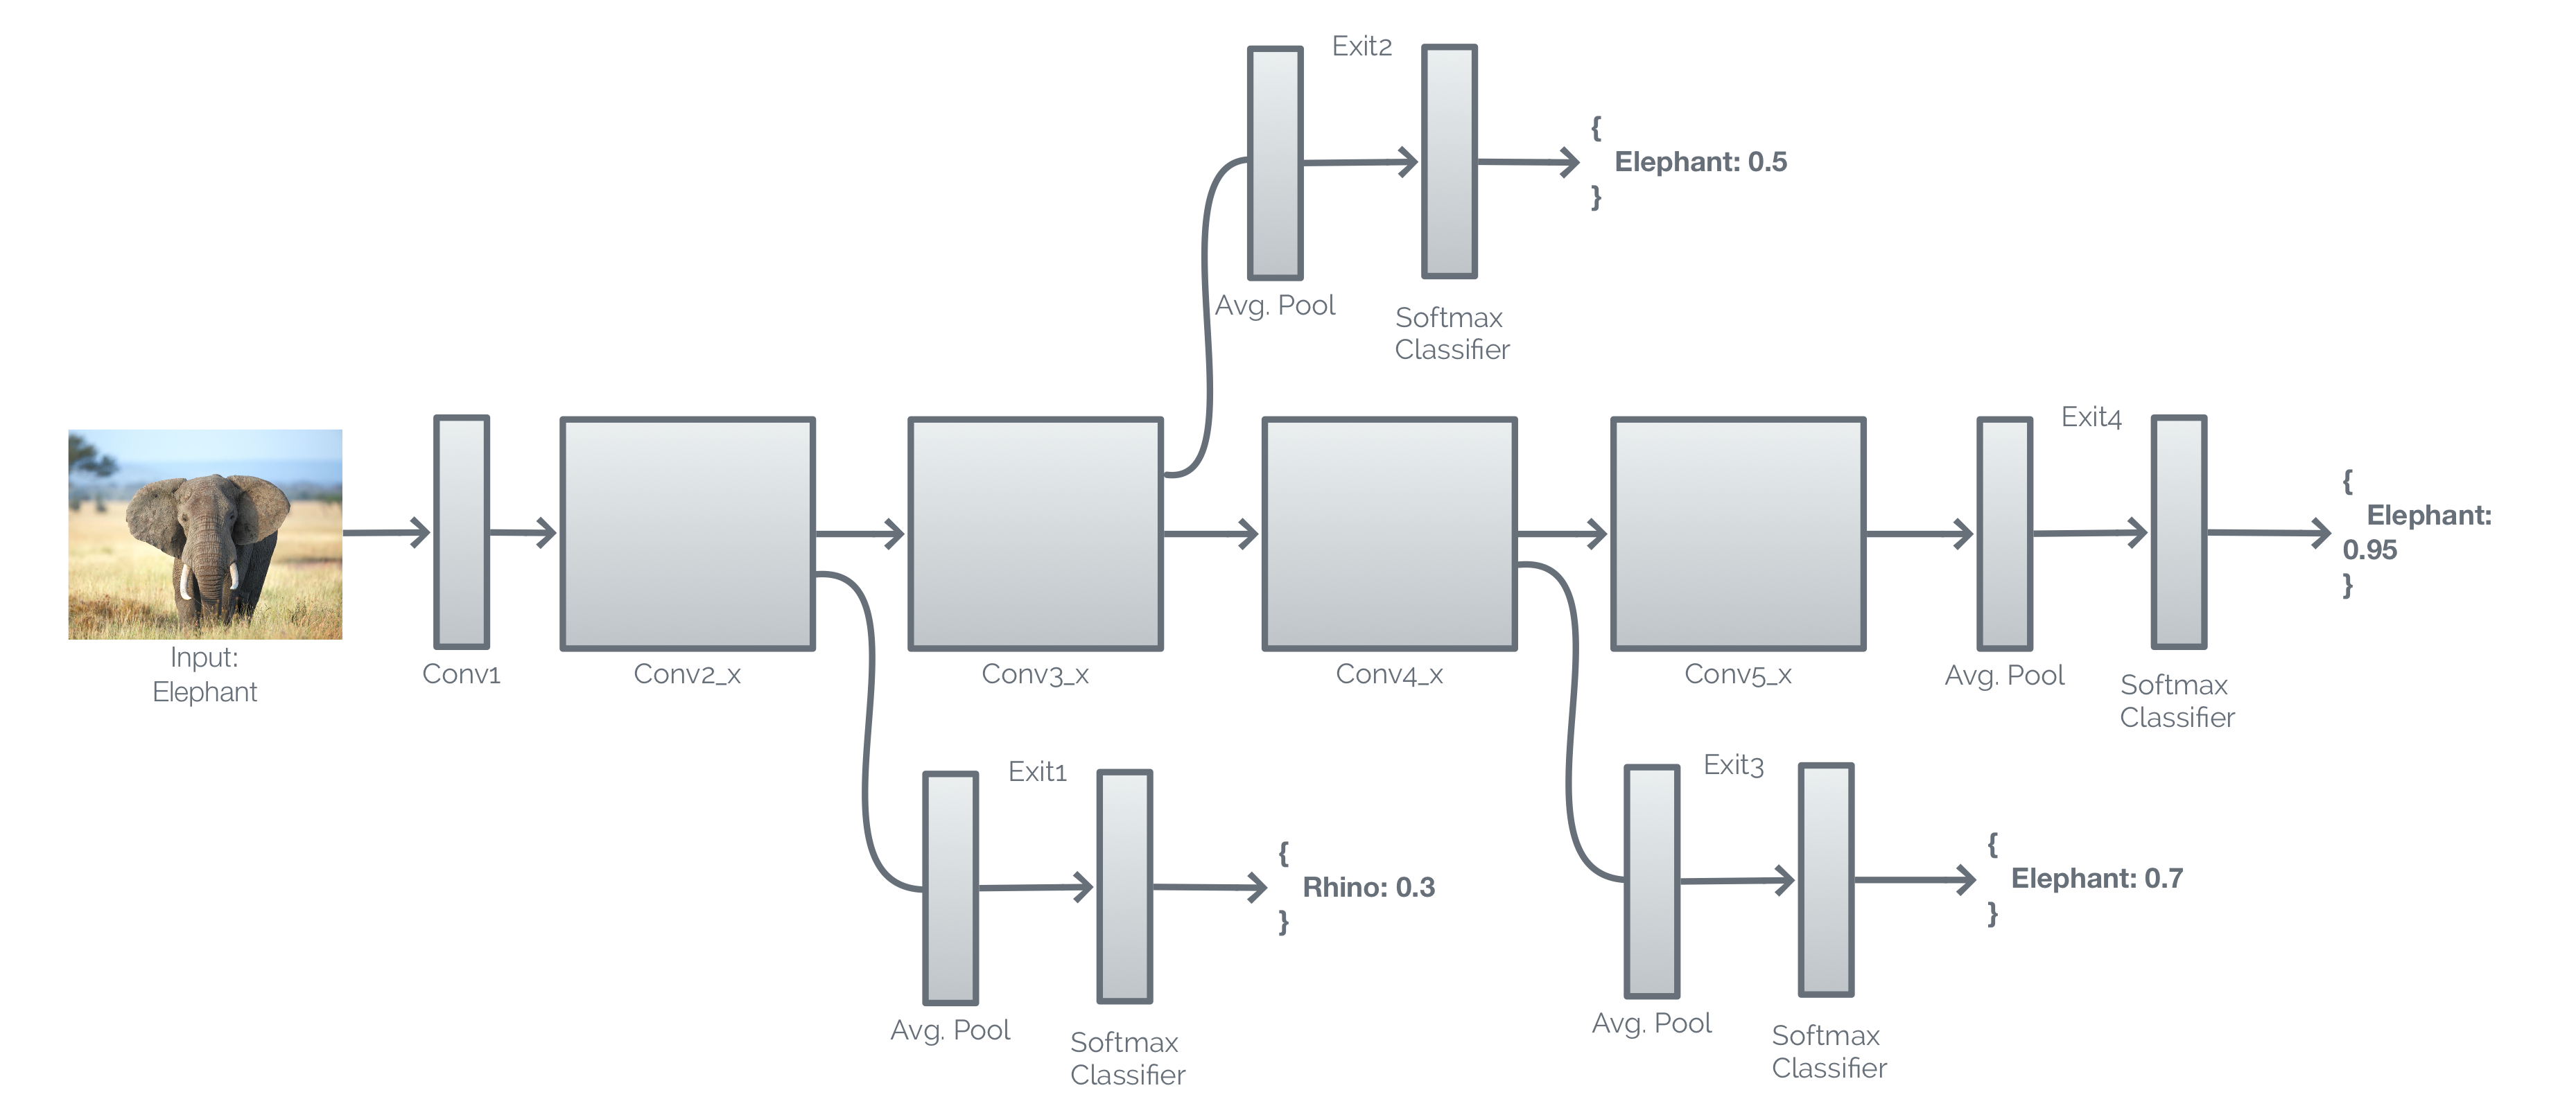
\includegraphics[width=\linewidth]{figures/models/BResNet}
	\caption[B-\gls{resnet} architecture]{Branchy-\gls{resnet}101: \gls{resnet}101 extended to implement the BranchyNet framework. The figure illustrates how classification confidence grows, as we go deeper in the model. The first exit actually fails to classify the elephant. }
	\label{fig:b-resnet}
\end{figure}


\subsection{Branchy-DenseNet}

In this section is the dense layers, the building block of the densely connected network, is explained. Followed by a design description of Branchy-\gls{densenet}.

DenseNet \cite{huang_densely_2016} is build on the assumption, that many layers of a \gls{resnet} only have a small contribution to the output and can in fact be dropped during training \cite{huang_densely_2016}. Instead of adding previously learned information to the output, \gls{densenet} combines features from all subsequent layers by concatenation, as there is no need to relearn redundant information. Figure \ref{fig:densenet} show the dense connections, that combine features from previous layers and how the features size grows throughout a densely connected block \todo{maybe a bit sharper explanation and more figure near.}

%\begin{figure}
%	\centering
%	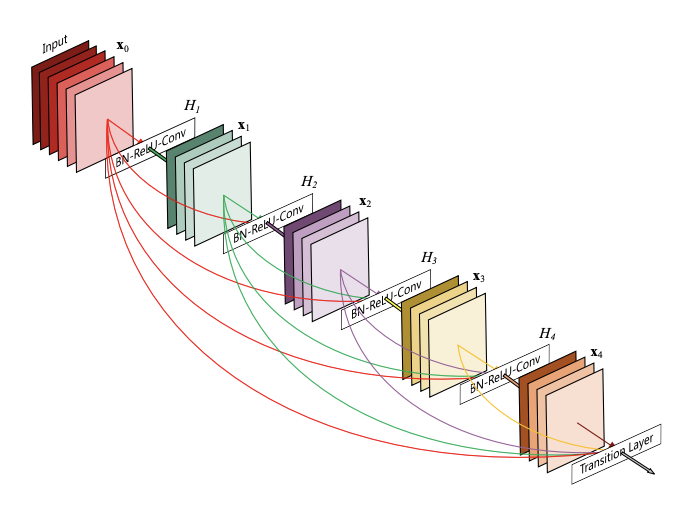
\includegraphics[width=.5\linewidth]{figures/models/denseblock}
%	\caption[Densely Connected Block]{Densely Connected Block}
%	\label{fig:denseblock}
%\end{figure}

The densely connected layers are similarly to residual network grouped into resolution block called dense blocks, but for \gls{densenet} intermediate transition layers are added between dense block to downsample the feature size. 

\begin{figure}
	\centering
	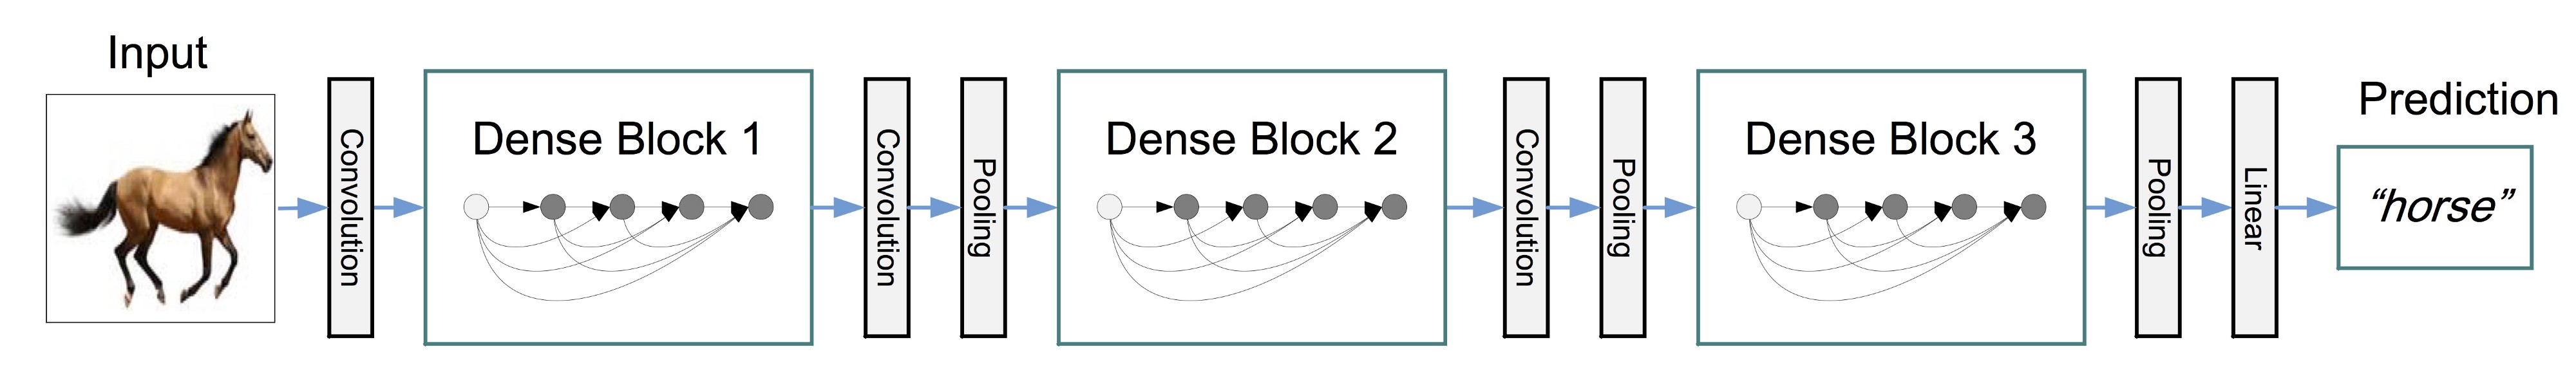
\includegraphics[width=\linewidth]{figures/models/densenet}
	\caption[Densely Connected Block]{Densely Connected Block}
	\label{fig:densenet}
\end{figure}

The collective knowledge from all preceding layers gives more diversified features compared to the correlated features of \gls{resnet}s. In \cite{huang_multi-scale_2017} the diversified features are shown to be more suited for early exiting,  as the information are better preserved using dense connection, hence even though information may have been collapsed to generate a short-term feature for the classifier. Thus placement of an intermediate classifier have less impact on the learned features for a later classifier. \gls{densenet} can be thinner as the number of channel can be fewer, thus more efficient compared to traditional and residual networks. Additionally densely connected blocks have a regularizing effect thus reducing overfitting the training data, hence perform better on smaller training sets. 

Table \ref{tbl:densenet121} describes the block and layers of the \gls{densenet} architecture. 

\small
\begin{minipage}[c]{\linewidth}
\begin{longtabu}{>{\bfseries}X|X[c]|X[2c]}
	\caption[\gls{densenet}-121 description]{\gls{densenet}-121 description. The table describes the blocks of \gls{densenet}-121. $k$ is the growth rate of the DenseBlock. A typical setting is $k=32$ yielding 256, 512 and 1024 output channels for denseblock(1-3) respectively. The transition layer downsamples the output channel by a factor of 2, thus the number of input channels for DenseBlock(2-4) becomes 128, 256 and 512 respectively.} \label{tbl:densenet121} \\
	\toprule
	\rowfont{\bfseries}
	Layers & Output size & Layer description \tabularnewline
	\hline
	\endfirsthead
	\multicolumn{3}{@{}l}{\textbf{\textcolor{black}{Table \ref{tbl:resnet50}:}} continued}\\
	\toprule
	\rowfont{\bfseries}
	Layers & Output size & Layer description \tabularnewline
	\hline
	\endhead % all the lines above this will be repeated on every page
	\hline
	\multicolumn{3}{@{}l}{continued \ldots}\\
	\endfoot
	\hline
	\endlastfoot
	Convolution & $112\times 112$& $7\times 7, \:\mathrm{stride}\: 2$ \tabularnewline \hline
	Pooling & $56\times 56$& $3\times 3, \:\mathrm{maxpool},\:  \mathrm{stride}\: 2$ \tabularnewline \hline
	\multirow{3}{*}{DenseBlock (1)} 	& \multirow{3}{*}{$56 \times 56$} & \multirow{3}{*}{
		$\begin{bmatrix}
		1 \times 1, k \\ 3 \times 3, k \\
		\end{bmatrix} \times 6$ }		\tabularnewline										
	& &  	\tabularnewline
	& & 	\tabularnewline
	\hline
	
	Transition  	& $56 \times 56$ & $1 \times 1\: \mathrm{conv}$ \tabularnewline \tabucline{2-3}							
	Layer (1) & $28\times 28$ & $2\times 2\: \mathrm{average\: pool,\: stride}\: 2$	\tabularnewline
	
	\hline
	
	\multirow{3}{*}{DenseBlock (2)} 	& \multirow{3}{*}{$28 \times 28$} & \multirow{3}{*}{
		$\begin{bmatrix}
		1 \times 1, k \\ 3 \times 3, k \\
		\end{bmatrix} \times 12$ }		\tabularnewline										
	& &  	\tabularnewline
	& & 	\tabularnewline
	\hline
	
	Transition  	& $28 \times 28$ & $1 \times 1\: \mathrm{conv}$ \tabularnewline \tabucline{2-3}							
	Layer (2) & $14\times 14$ & $2\times 2\: \mathrm{average\: pool,\: stride}\: 2$	\tabularnewline
	
	\hline
	
	\multirow{3}{*}{DenseBlock (3)} 	& \multirow{3}{*}{$14 \times 14$} & \multirow{3}{*}{
		$\begin{bmatrix}
		1 \times 1, k \\ 3 \times 3, k \\
		\end{bmatrix} \times 24$ }		\tabularnewline										
	& &  	\tabularnewline
	& & 	\tabularnewline
	\hline
	
	Transition  	& $14 \times 14$ & $1 \times 1\: \mathrm{conv}$ \tabularnewline \tabucline{2-3}							
	Layer (3) & $7\times 7$ & $2\times 2\: \mathrm{average\: pool,\: stride}\: 2$	\tabularnewline
	
	\hline
	
	\multirow{3}{*}{DenseBlock (4)} 	& \multirow{3}{*}{$7 \times 7$} & \multirow{3}{*}{
		$\begin{bmatrix}
		1 \times 1, k \\ 3 \times 3, k \\
		\end{bmatrix} \times 16$ }		\tabularnewline										
	& &  	\tabularnewline
	& & 	\tabularnewline
	\hline
	
	Classification  	& $1 \times 1$ & $7 \times 7\: \mathrm{global\: average\: pool}$ \tabularnewline \tabucline{2-3}							
	Layer &  \multicolumn2{c}{$\mathrm{Avg.\: Pool,\:} 1000d\: \mathrm{fc,\: Softmax}$} \tabularnewline
	\bottomrule
\end{longtabu}
\color{caption-color}{\textit{Source: \citetitle{huang_densely_2016}, by \citeauthor{huang_densely_2016} \cite{huang_densely_2016}, describes a full list of Densely Connected Networks (\gls{densenet}-121, \gls{densenet}-169, \gls{densenet}-201 and \gls{densenet}-264)}} \color{main-color}
\end{minipage}

In the same fashion as \gls{bresnet}'s, the exits are placed after a densely connected block to obtain feature of sufficient quality and exiting as quickly as possible. If used in Edge-Device mode and the confidence was insufficient the transition layer after the DenseBlock is executed, before data is being preprocess for offloading. \todo{reformulate}

\begin{figure}
	\centering
	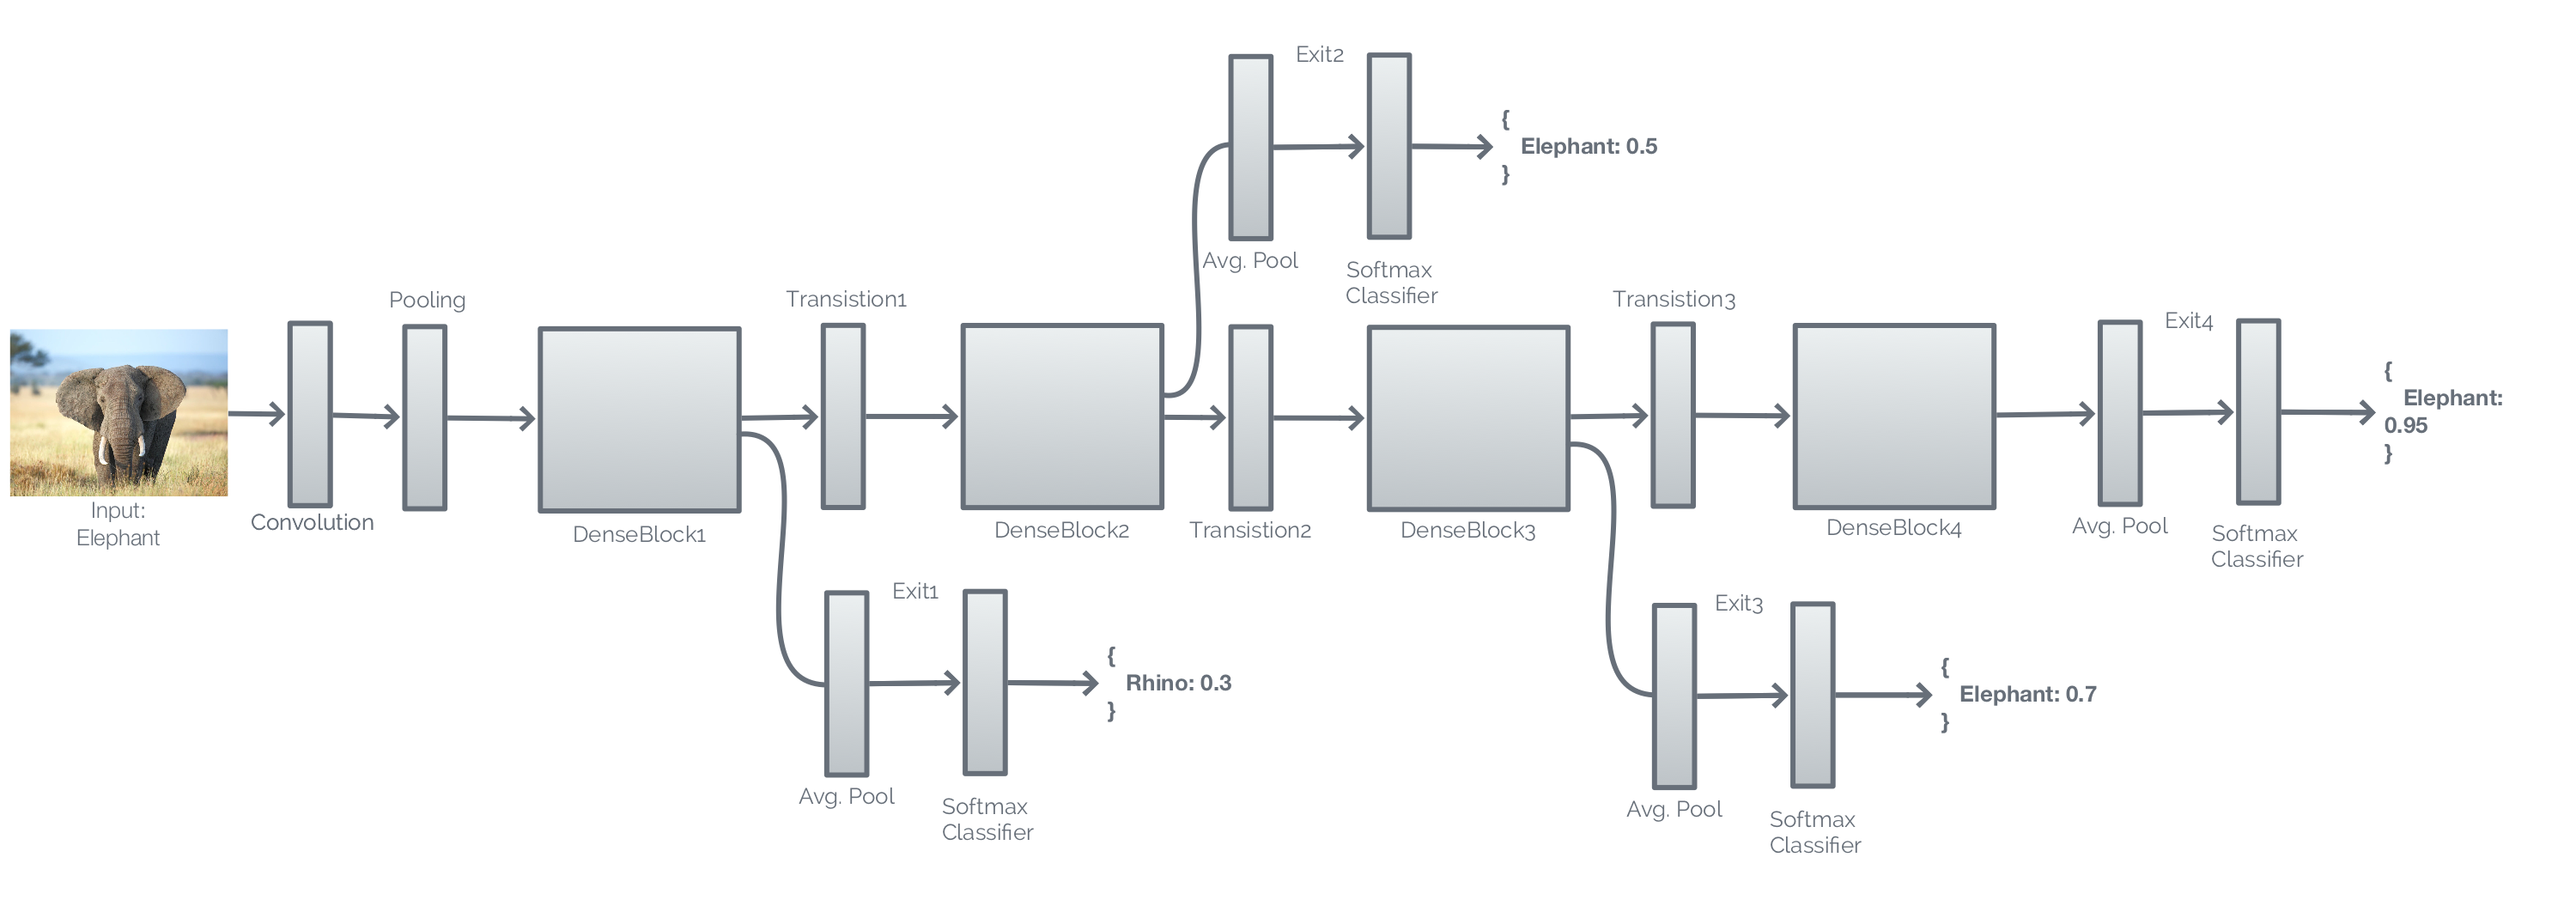
\includegraphics[width=\linewidth]{figures/models/b-densenet}
	\caption[B-\gls{densenet} architecture]{\gls{bdensenet}: \gls{densenet}-121 extended to implement the \gls{branchynet} framework. The figure illustrates how classification confidence grows, as we go deeper in the model. The first exit actually fails to classify the elephant. }
	\label{fig:b-densenet}
\end{figure}

\section{Experimental Setup} \label{sec:ee-exp-setup}

All code is written in \gls{python} 3.7 \cite{van_rossum_python_1995} using the \gls{pytorch} 1.2
framework \cite{paszke_automatic_2017} and using the \gls{torchvision} 0.4 library \cite{marcel_torchvision_2010}. All code is available at:
{\color{sns-grey}\url{https://github.com/AlexKarlsen/thesis-src}}. 

Table \ref{tbl:platforms} lists the hardware and its characteristics used for the experiments. Table \ref{tbl:models} lists the models used in the experiment and compares the number of layers, parameters and \gls{flop}s of the models. The number of parameters and \gls{flop}s have been found using \gls{thop} \cite{zhu_thop_nodate}, by inference a random 4d tensor of size $ (\mathrm{batch,channels,width,height})=(1,3,224,224) $ to all models.
 
\begin{longtabu}{>{\bfseries}X[0.8]|X[0.8]|X[1.5]|X[r0.3]}
	\caption[Platform hardware comparison]{Platform hardware comparison of Window 10 Stationary PC and NVIDIA Jetson TX2 Edge Computer} \label{tbl:platforms} \\
	\toprule
	\rowfont{\bfseries}
	Platform & CPU & GPU & RAM  \tabularnewline
	\bottomrule
	\endfirsthead
	\multicolumn{3}{@{}l}{\textbf{\textcolor{black}{Table \ref{tbl:platforms}:}} continued}\\
	\toprule
	\rowfont{\bfseries}
	Platform & CPU & GPU & RAM  \tabularnewline
	\bottomrule
	\endhead % all the lines above this will be repeated on every page
	\bottomrule
	\multicolumn{3}{@{}l}{continued \ldots}\\
	\endfoot
	\hline
	\endlastfoot
	GPU Workstation	& Intel i5-6600K.	& NVIDIA GeForce GTX 1080, 2560 CUDA cores	& 16GB \tabularnewline
	\hline
	Jetson TX2	& ARM Cortex-A57 	& NVIDIA Pascal GPU, 256 CUDA cores 		& 8GB \tabularnewline
	\hline
	NUC		  	& Intel i7-7567U	& None										& 16GB \tabularnewline									
	\bottomrule
\end{longtabu}%equipped with a NVIDIA GeForce 1080 GTX \gls{gpu} using CUDA 10.1 and cuDNN 7.6.3.
\begin{longtabu}{>{\bfseries}X|X[r]|X[r]|X[r]}
	\caption[Model comparison]{ Model Parametric Comparison. The B-\gls{densenet} and \gls{msdnet} drastically reduces the mount of parameters and G\gls{flop}s compared to B-\gls{resnet}. The early exit models should be able to reduce inference delay, as they need less parameters and \gls{flop}s.}\label{tbl:models} \\
	\toprule
	\rowfont{\bfseries}
	Model  & Layers & Parameters (M) & G\gls{flop}s \tabularnewline
	\hline
	\endfirsthead
	\multicolumn{3}{@{}l}{\textbf{\textcolor{black}{Table \ref{tbl:models}:}} continued}\\
	\toprule
	\rowfont{\bfseries}
	Model & Layers & Parameters (M) & G\gls{flop}s \tabularnewline
	\hline
	\endhead % all the lines above this will be repeated on every page
	\hline
	\multicolumn{3}{@{}l}{continued \ldots}\\
	\endfoot
	\hline
	\endlastfoot
	ResNet & $ 101 $ & $ 42.705 $ & $ 7.864 $ \tabularnewline
	\hline
	DenseNet & $ 121 $ & $ 7.056 $ & $ 2.897 $ \tabularnewline
	\hline
	B-ResNet & $ 104 $ & $ 42.885 $ & $ 7.866 $ \tabularnewline 
	\hspace{3mm} Exit-0  & 11 &   0.251 & 0.807 \tabularnewline
	\hspace{3mm} Exit-1  & 13 &   1.270 & 1.041 \tabularnewline
	\hspace{3mm} Exit-2  & 70 &  26.193 & 5.206 \tabularnewline
	\hspace{3mm} Exit-3  & 11 &  15.170 & 0.812 \tabularnewline
	\hline
	B-DenseNet & $ 124 $ & $ 7.236 $ & $ 2.898 $\tabularnewline
	\hspace{3mm} Exit-0  & 14 & 0.370 & 1.183  \tabularnewline
	\hspace{3mm} Exit-1  & 26 & 1.004 & 0.836  \tabularnewline
	\hspace{3mm} Exit-2  & 50 & 3.072 & 0.668  \tabularnewline
	\hspace{3mm} Exit-3  & 34 & 2.789 & 0.211  \tabularnewline
	\hline
	MSDNet & $ 25 $ & $ 23.958 $ & $ 1.374 $ \tabularnewline
	\hspace{3mm} Exit-0  & 5 & 4.239 & 0.345 \tabularnewline
	\hspace{3mm} Exit-1  & 5 & 4.534 & 0.349 \tabularnewline
	\hspace{3mm} Exit-2  & 5 & 4.301 & 0.325 \tabularnewline
	\hspace{3mm} Exit-3  & 5 & 3.675 & 0.248 \tabularnewline
	\hspace{3mm} Exit-4  & 5 & 7.210 & 0.107 \tabularnewline
	\bottomrule
\end{longtabu}


\begin{enumdescript}
	\item[Training] All training of the models of table \ref{tbl:models} have been accomplished using the \gls{gpu}-workstation of table \ref{tbl:platforms}. In each epoch the training- and validation-, -loss and -accuracy have been logged and used for analysis in section \ref{sec:ee-results}. The trained models are available at: {\color{sns-grey}\url{https://drive.google.com/open?id=1EAl9qGxcm2U3kPhEsHp0HotgNn_LMWa1}}.
	The listed and described training hyperparameters have been used for all training sessions. 
	
	\begin{enumdescript}
		\item[Epochs] An epoch is a step of training in which every training sample have been presented to the model. A training time of 50 epochs have been selected to limit overall training time to give time for multiple attempts and training multiple model.
		
		Training the models on the available hardware took $\sim$30 to  $\sim$40 hours depending on the model. In total 5 models have been fully trained once the rest of training settings had been found.
		
		\item[Early Stopping] Early stopping is finding the best obtained model by alternating between training and validation phases for each epoch. The best model is the one obtaining the highest accuracy on the validation data. Early stopping is a mechanism to avoid overtraining a model, that then overfits the training data and obtain poor validation accuracy. For \gls{branchynet} we use the model with the highest average accuracy to not favor any part of the model.  
		
		\item[Exit Weights] The same unit weights have been selected for all exits of the model again not to favor any part of the model. In \cite{teerapittayanon_branchynet:_2016} they claim, that putting more weight on early branches have a regularizing impact on the later classifiers and can actually achieve better performance. However, they too have chosen the same unit weights for all branches, for comparison of multiple models and avoid time consuming search for specific branch weights on a per model basis.
		
		\item[Optimizer] The weights of \gls{dnn}s are typically trained using a variant of \gls{sgd} \cite{goodfellow_deep_2016}. \gls{sgdr} \cite{loshchilov_sgdr:_2016} have shown faster convergence on a number of datasets, due to its ability to escape local minimas. It follows a cyclic learning rate schedule in contrast to former decaying learning rate schedules. It has shown, in general, to perform better than adaptive optimizers such as Adam \cite{kingma_adam:_2014}, which implement adaptive learnining rate to avoid being stuck in local minimas. 
		
		\gls{sgdr} uses an aggressive cosine annealing schedule with warm restarts. Figure \ref{fig:cosineannealing} illustrates the learning rate schedule.
		
		\begin{minipage}[t]{\linewidth}
			\centering
			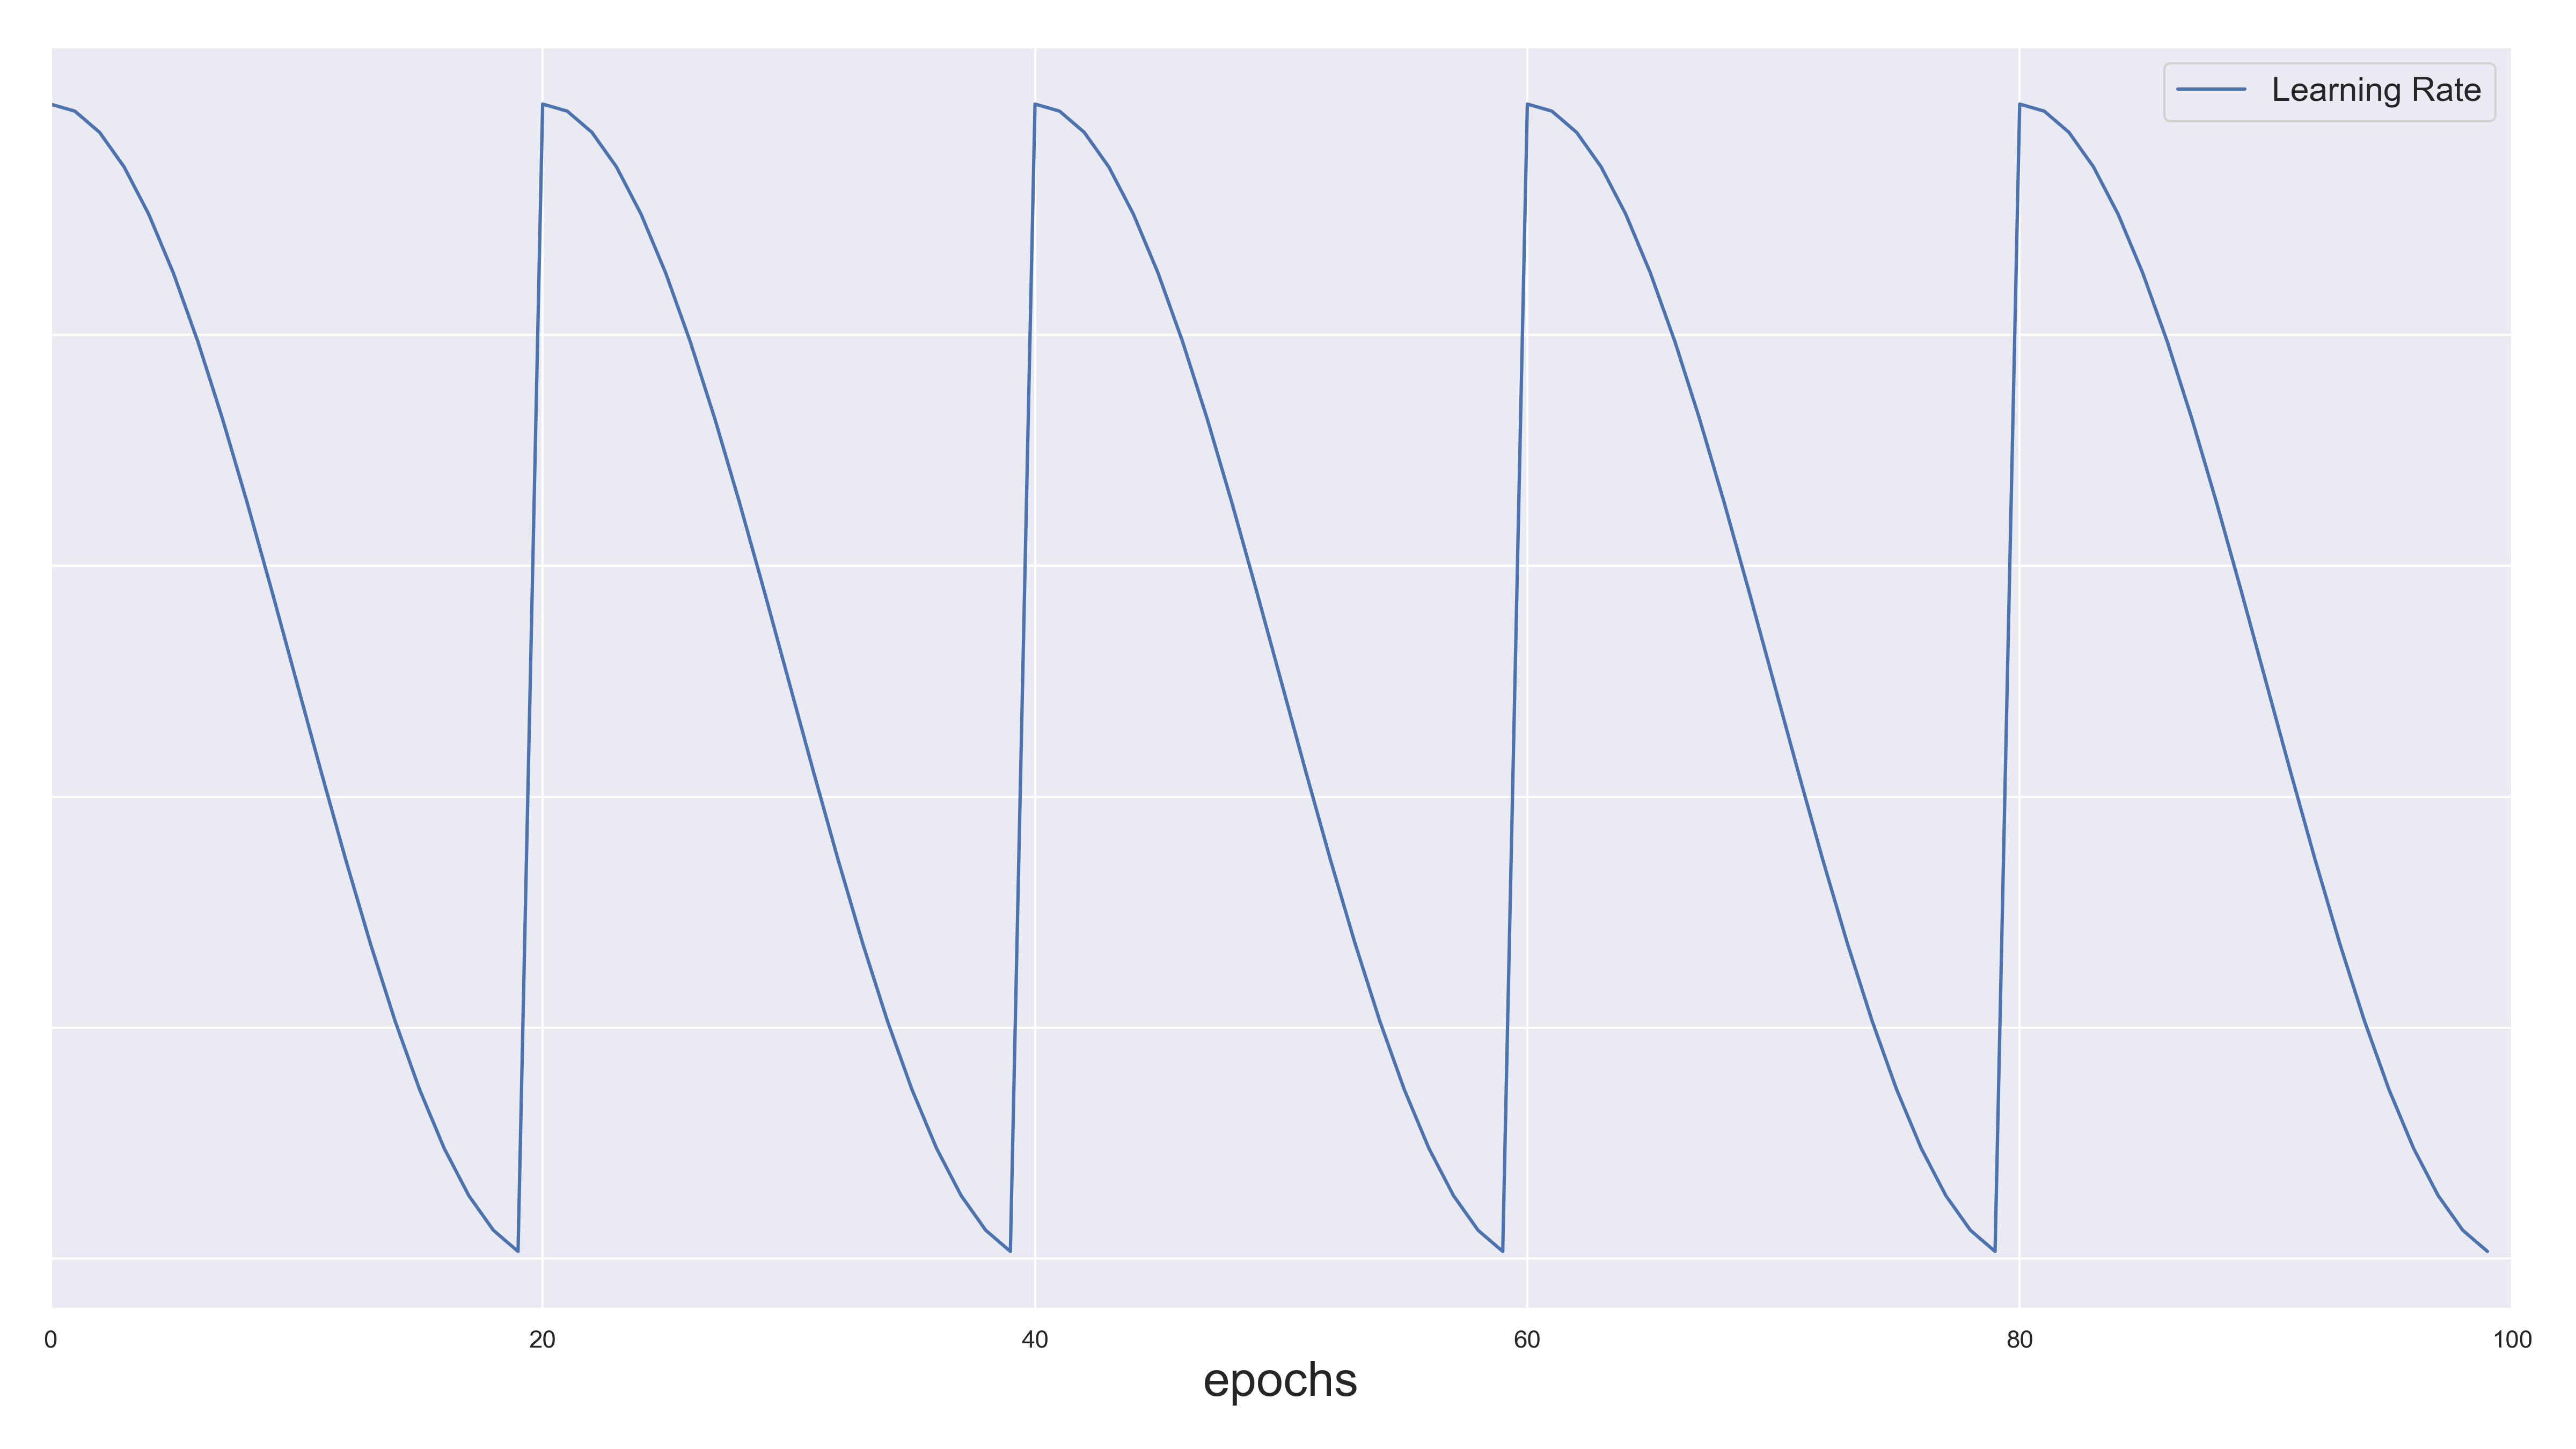
\includegraphics[width=.7\linewidth]{figures/lr.png}
			\captionof{figure}[Cosine Annealing Learning Rate]{Cosine Annealing Learning Rate} 
			\label{fig:cosineannealing}
		\end{minipage}
		
		\item[Batch Size] Batch Size are recommend to be between 1 and a few hundreds \cite{bengio_practical_2012}. To better utilize \gls{gpu}s a batch size in the power of 2 gives better runtime, e.g. 32 to 256 \cite{goodfellow_deep_2016}. Larger batch sizes have been driving by advancements in parallelism \cite{dean_large_2012}, which can improve the training time, however smaller batch size, have shown better generalization performance due to a regularizing effect \cite{masters_revisiting_nodate}, which especially large model, that tends to overfit can benefit from \cite{goodfellow_deep_2016}. 
		
		A batch size of 16 was found to be the maximum power of 2 possible with the computational budget of 8Gb RAM. The standard choice of 32 caused memory exhaustion. However, a batch size of 16 provide decent training times and may provide additional regularization over 32. Smaller batch sizes were not experimented with due to time constraints. The batch size of 16 was chosen for all \gls{dnn} training sessions.
		
		\item[Datasets] \gls{min100} is a subset of the \gls{ilsvrc2012} dataset \cite{russakovsky_imagenet_2015} created for this project, to reduce training time from several weeks to only days on available hardware. The subset is inspired by MiniImageNet \cite{vinyals_matching_2016}, that uses a subset of 100 classes with 600 samples for each class. \gls{min100} contains 100 out of 1.000 randomly sampled classes, which gives 127.300 out of 1.2m training samples and 5.000 out of 50.000 validation samples. A full list of classes are found in the table \ref{tbl:min100}. 
		
		Compared to other sufficiently dense classification datasets e.g \gls{tinyimagenet} \cite{li_cs231n:_2018}, \gls{cifar10} and \gls{cifar100} \cite{krizhevsky_cifar-10_nodate}, the image sizes of these datasets are respectively $(64\times 64$), $(32\times 32)$, $(32\times 32)$ pixels, all of which are considered too small for this project. Other datasets such as MS COCO and Pascal VOC are better suited for object detection/segmentation, as images are not cropped to only focus on a single object, thus too challenging for classification. In fact Pascal VOC was initially tested, the model however, clearly overfitted the training data due to data sparsity. 
		
		\item[Image Augmentation] A models ability generalize a specific classification problem has a close connection with the number of available training samples. Data augmentation haven proven to be powerful tool in order to virtually create more training data \cite{perez_effectiveness_2017}. Enlarging a training dataset by data augmentation can help create new versions of an image, that are different from but still similar to the original image, without actually having to acquire and annotate new samples \cite{goodfellow_deep_2016}.  
		
		\begin{minipage}[t]{\linewidth}
			\centering
			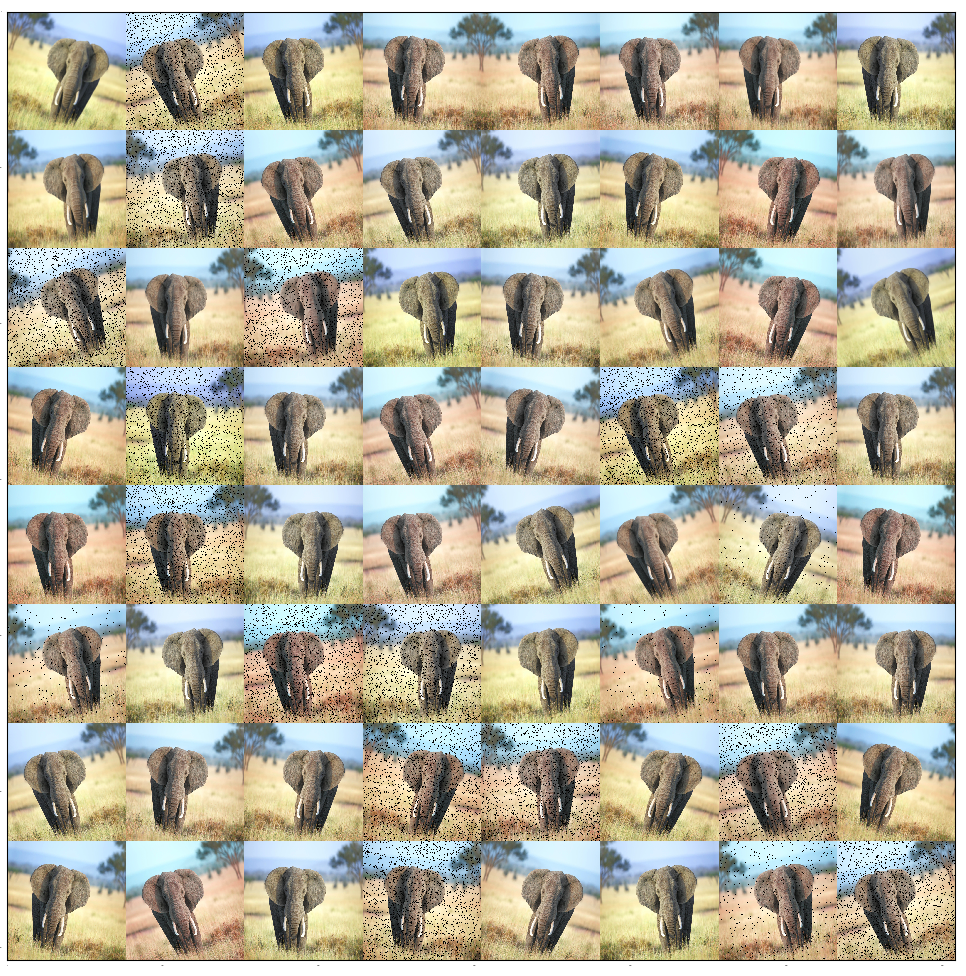
\includegraphics[width=.7\linewidth]{figures/augmentation/augmentation_high_resolution.png}
			\captionof{figure}[Image Augmentaion Example]{Image Augmentation of an elephant}
			\label{fig:augmentation}
		\end{minipage}
		
		Image augmentation involves transformations using tools from image processing to randomly apply noise injection, and color space transformations including contrast and saturation distortions, as well as geometric transformations, such as simple transformations of flipping the image to more complex affine transformations to create different image perspectives \cite{shorten_survey_2019}. Figure \ref{fig:augmentation} shows 64 random augmentations of an image of an elephant, achieved using \gls{imgaug} \cite{jung_imgaug:_nodate}. 
		
		New methods have been proposed where image transformations are learned to improve generalization e.g. AutoAugment \cite{cubuk_autoaugment:_2018}. 
		
		Other methods involves actually enlarging the training dataset by synthetically creating more data using a \gls{gan}. \gls{gan}s can help overcome limited data given the available training data or a 3D model, by artificially constructing synthetic samples in different background, light setting and from alternate perspectives.
		
		Methods that do not cover enriching the available training, but alters the learning procedure are called regularization and covers; weight decay, dropout, batch normalization etc. We do not experiment with these regularization technique, but uses the settings set in the implementation of the models.
		
		\item[Transfer Learning] Transfer learning is the procedure of using a pre-trained model to train on a new dataset, under the assumption, that features learned on one image dataset can be reused for another dataset \cite{yosinski_how_2014}. Typically models have been pre-trained on the ImageNet dataset. The density of the dataset enables models to learn general features suitable for other domains \cite{kornblith_better_2019}. Transfer learning are especially suited for when the new data domain is of limited quantity and the similarities between the two data domains are strong. If the similarity is weak a model can be partially trained, the shallow layers containing general features are frozen and only the deeper layers with more specialized features are fine-tuned for the new data domain \cite{li_cs231n:_2018}. Thus, transfer learning can reduce the training time to learn general features of shallow layers and possibly learn more specific features at deeper layers, adapted to the new dataset.
	\end{enumdescript}
	
	\item[Inference] The inference experiment have been conducted by letting all samples inference the model, the output and measured time of all exits have been logged and used for analysis in section \ref{sec:ee-results}. All hardware of table \ref{tbl:platforms} and all trained models of table \ref{tbl:models} have been used. The inference experiment does not require nearly the same amount of setting as the training does, those required are listed here:
	\begin{enumdescript}
		\item[Batch Size] A batch size of 1 have been chosen to simulate a real scenario, and to measure time of each samples
		\item[Dataset] The validation dataset of \gls{min100} containing 5000 samples have been used.
	\end{enumdescript} 
	
\end{enumdescript}

In the next section we present the results of our experiments with early exiting and conventional models.

\section{Results} \label{sec:ee-results}

The results section consists of two main parts. The first one covers the result from training the \gls{dnn}s. The second part covers experimentation using our trained networks. 

\subsection{Training Results}

We trained the three early exiting models \gls{bresnet}, \gls{bdensenet} and \gls{msdnet}, along with conventional versions of the \gls{resnet}101 and \gls{densenet}-121. The \gls{dnn}s were trained on the \gls{min100} training set..

First we trained {bresnet} using transfer learning from the ImageNet dataset. We froze the features of the network and only trained the classifiers of all the exits. Figure \ref{fig:frozen-b-resnet-miniimagenet-100} show the results from the training. The figure shows, that the features learned from a conventional single exit model, are not suitable for an early exit model. None of the intermediate classifiers are able to obtain acceptable accuracy on neither the training nor the validation set. The features for the shallower part of the network are not optimized for the early classifiers. This study clearly reveals the need to train the entire model, to obtain an early exit model with decent accuracy.  

\begin{figure}
	\centering
	\captionsetup[subfigure]{justification=centering, farskip=1pt,captionskip=1pt}
	
\includegraphics[width=.5\textwidth]{figures/training_plots/frozen_b-resnet_exit_legend}
	\subfloat[Train loss\label{fig:frozen-b-resnet-train-loss}]{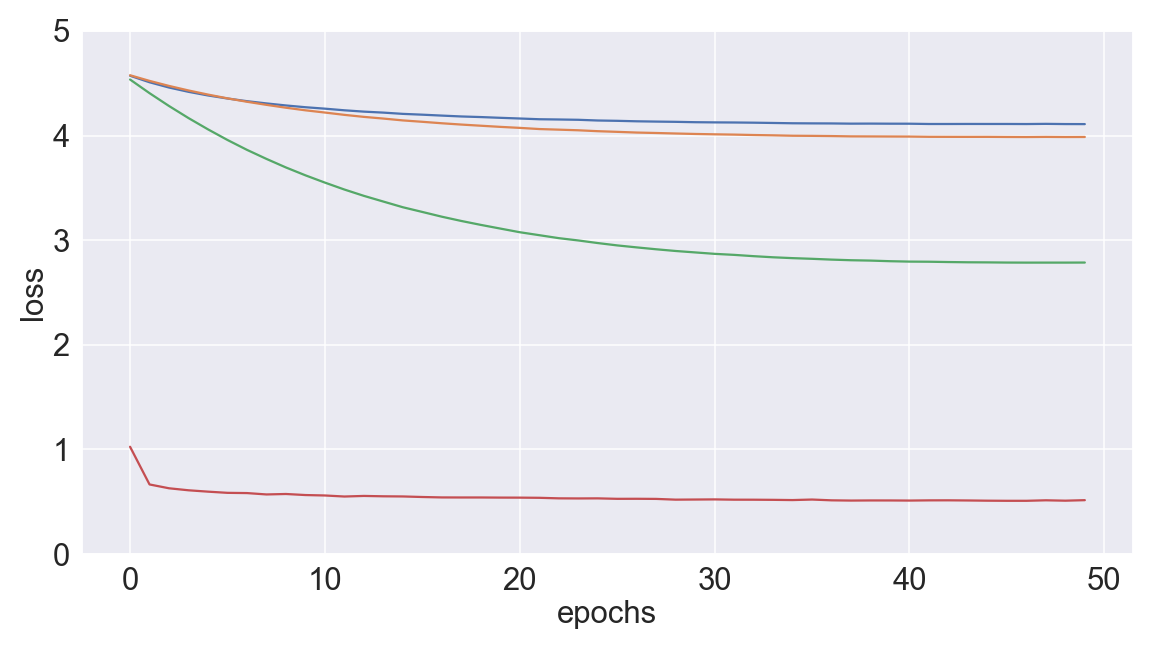
\includegraphics[width=.49\textwidth]{figures/training_plots/frozen_b-resnet_train-loss}}
	\subfloat[Test loss \label{fig:frozen-b-resnet-test-loss}]{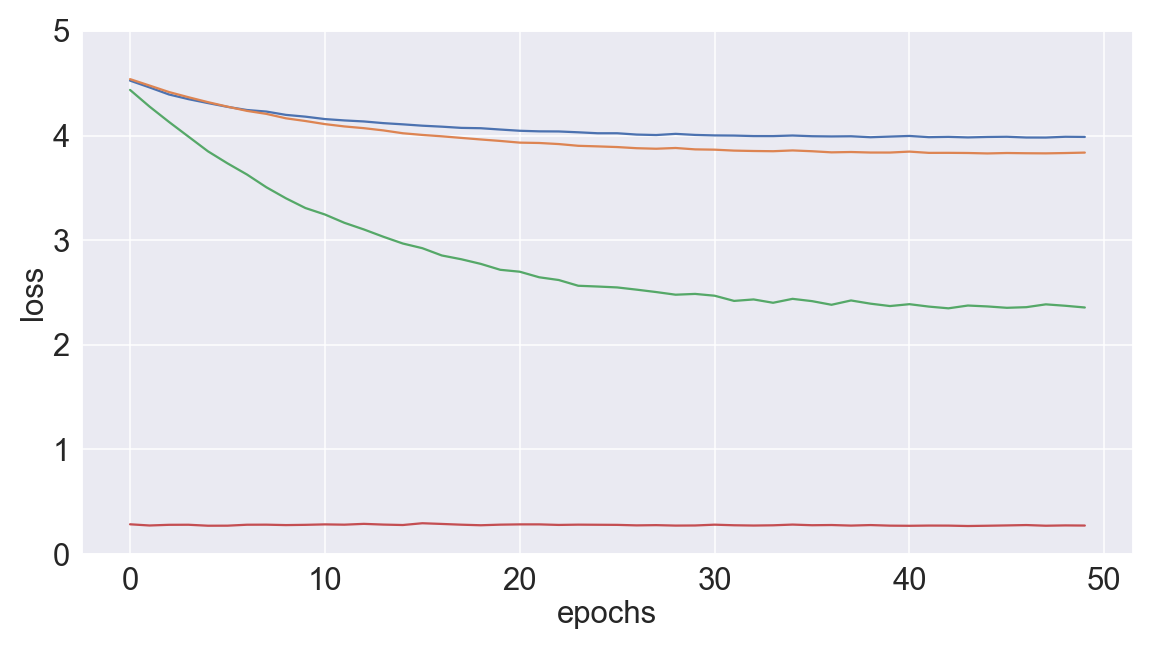
\includegraphics[width=.49\textwidth]{figures/training_plots/frozen_b-resnet_test-loss}}
	\hfill
	\subfloat[Train accuracy\label{fig:frozen-b-resnet-train-acc}]{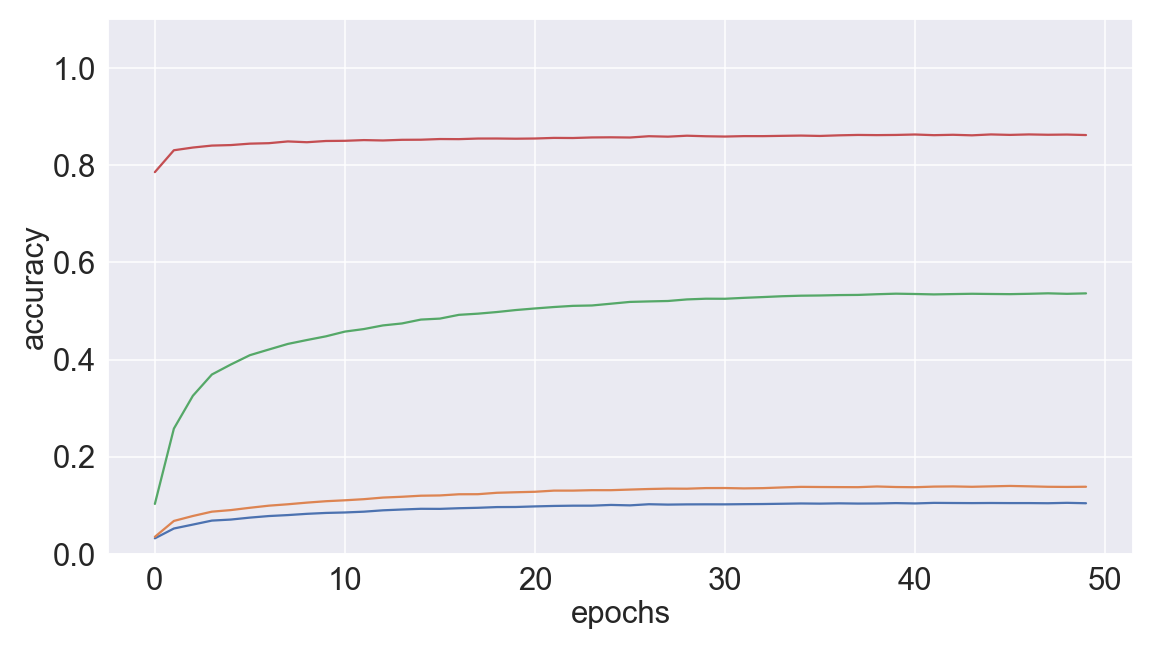
\includegraphics[width=.49\textwidth]{figures/training_plots/frozen_b-resnet_train-accuracy}}
	\subfloat[Test accuracy\label{fig:frozen-b-resnet-test-acc}]{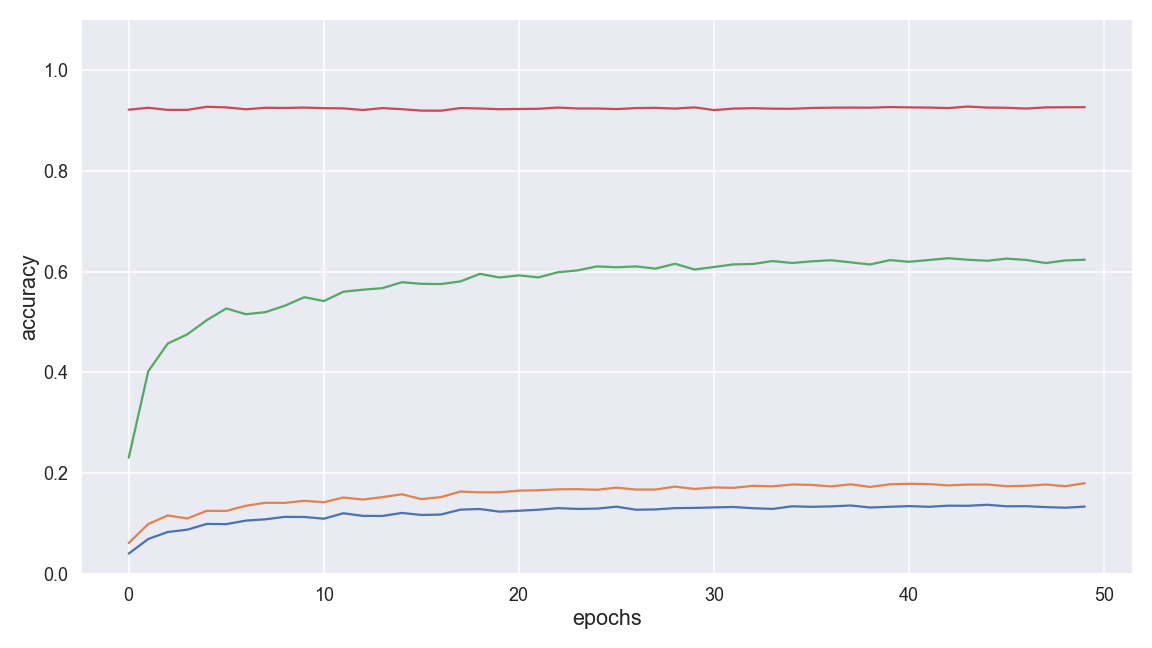
\includegraphics[width=.49\textwidth]{figures/training_plots/frozen_b-resnet_test-accuracy}}
	\caption[Frozen Bresnet Training summary]{Frozen \gls{bresnet} Training summary: shows the progression of model attributes over times of epochs, \protect\subref{fig:frozen-b-resnet-train-loss} train loss, \protect\subref{fig:frozen-b-resnet-test-loss} test loss, \protect\subref{fig:frozen-b-resnet-train-acc} train accuracy, \protect\subref{fig:frozen-b-resnet-test-acc}, test accuracy.}
	\label{fig:frozen-b-resnet-miniimagenet-100}
\end{figure}

As found in \cite{teerapittayanon_branchynet:_2016}, we unfreeze the model, to allow the features of the model to be optimized for the intermediate classifiers of the early exit model. Figure \ref{fig:b-resnet-miniimagenet-100} show the training results. The accuracy at early exits classifiers are greatly improved by 140 \% to almost 390 \%. However, the accuracy of the final classifier are reduced by 4 \%. The reduction in accuracy may be caused by;
\begin{enumerate}
	\item The features of the third and largest resolution block just before exit-2, see table \ref{tbl:resnet101}, may be optimized too much for exit-2, thus collapses the information, that the last block should use to learn more descriptive features. 
	\item It could be a sign of overfitting, due to the size of dataset is only $\frac{1}{10}$ of the dataset used to train the original model. 
\end{enumerate}
However, the last two exits obtain a training accuracy close to 1. However, there is no notable degradation in validation loss or accuracy, which would have been the clearest sign of overfitting. We did also train conventional versions of the two models on the same datasets, and since both models are able to obtain over 0.9 in accuracy, we argue, that the most probable reason is optimization to earlier exit, as the same trend is shown in \cite{huang_multi-scale_2017}.

\begin{figure}
	\centering
	\captionsetup[subfigure]{justification=centering, farskip=1pt,captionskip=1pt}
	
\includegraphics[width=.5\textwidth]{figures/training_plots/b-resnet_exit_legend}
	\subfloat[Train loss\label{fig:b-resnet-train-loss}]{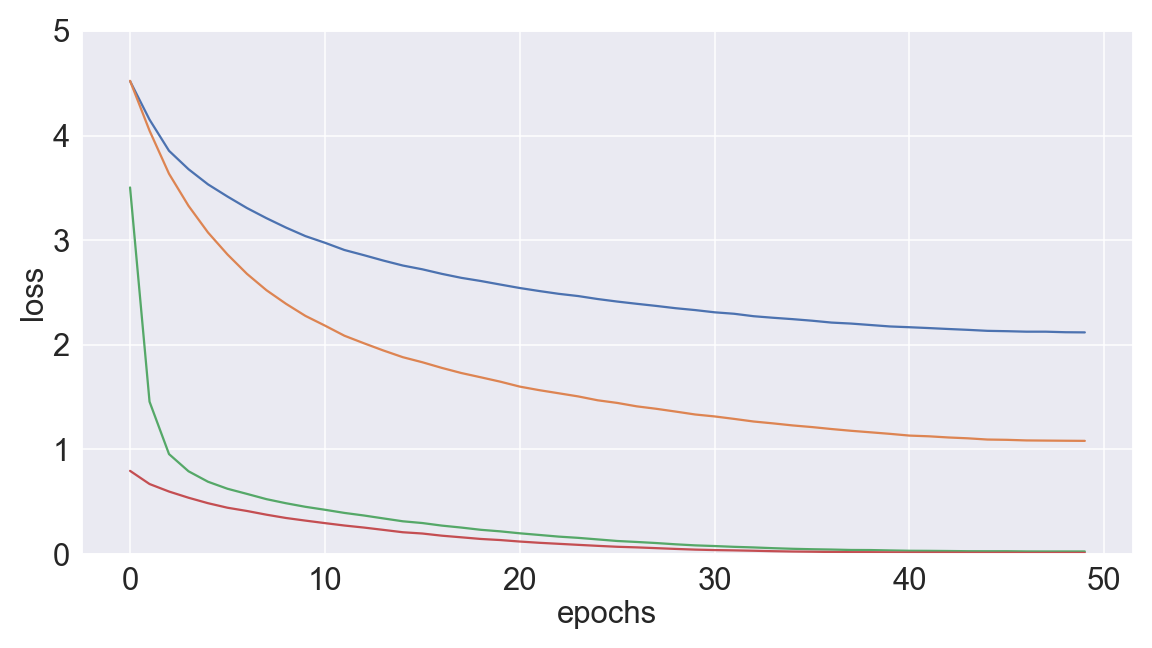
\includegraphics[width=.49\textwidth]{figures/training_plots/b-resnet_train-loss}}
	\subfloat[Test loss \label{fig:b-resnet-test-loss}]{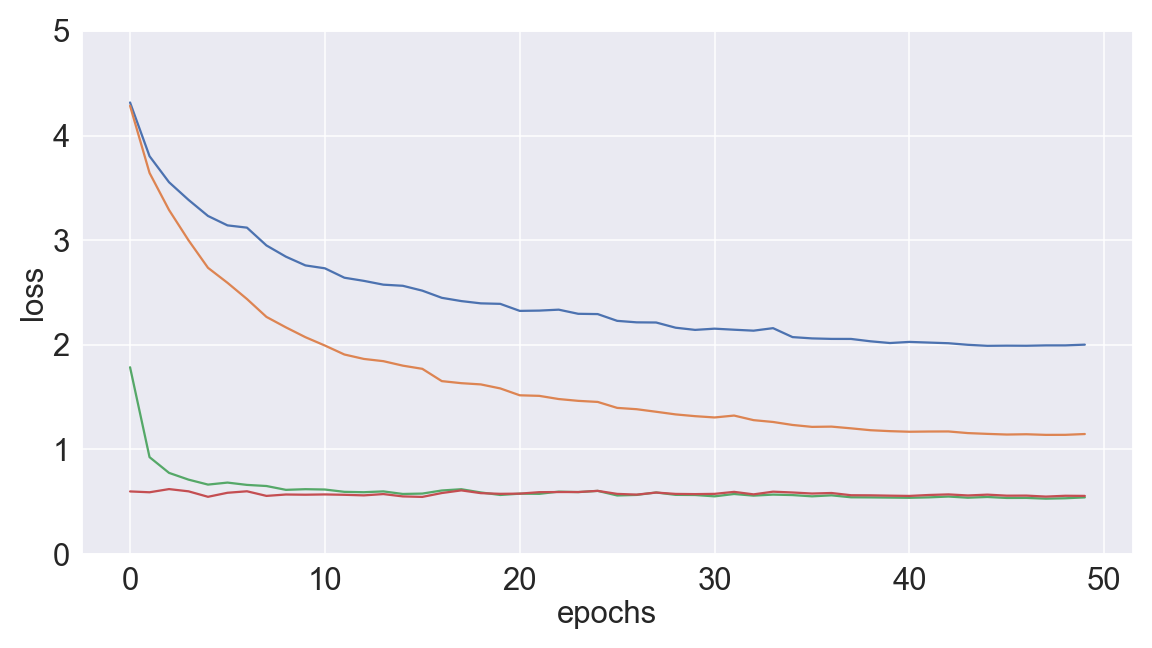
\includegraphics[width=.49\textwidth]{figures/training_plots/b-resnet_test-loss}}
	\hfill
	\subfloat[Train accuracy\label{fig:b-resnet-train-acc}]{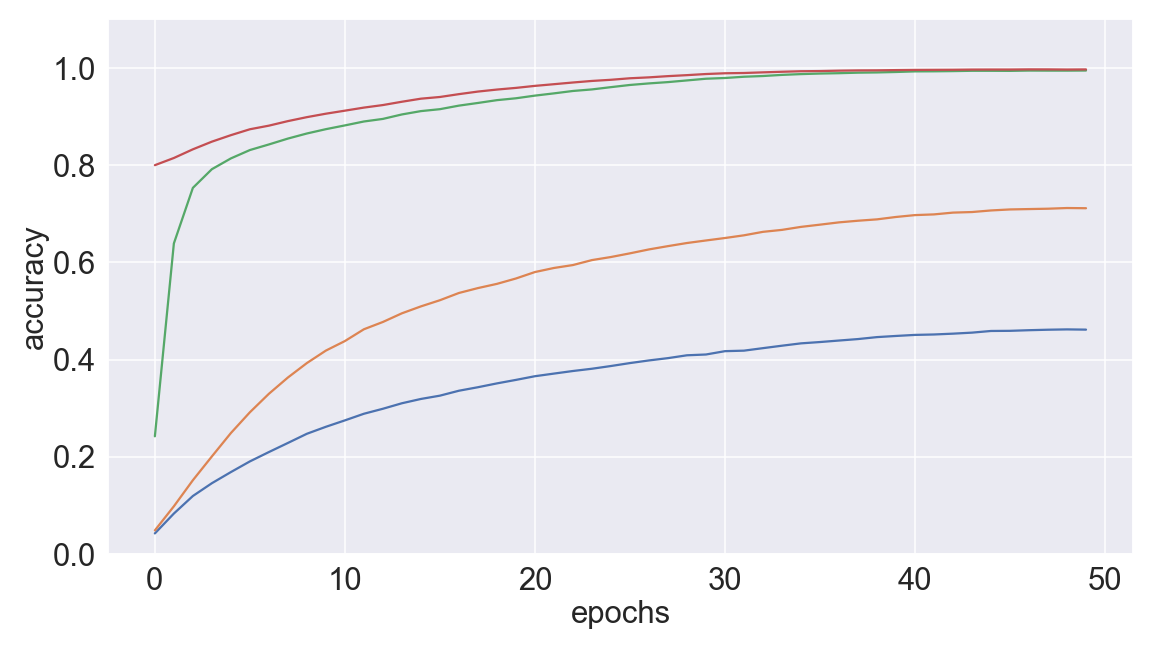
\includegraphics[width=.49\textwidth]{figures/training_plots/b-resnet_train-accuracy}}
	\subfloat[Test accuracy\label{fig:b-resnet-test-acc}]{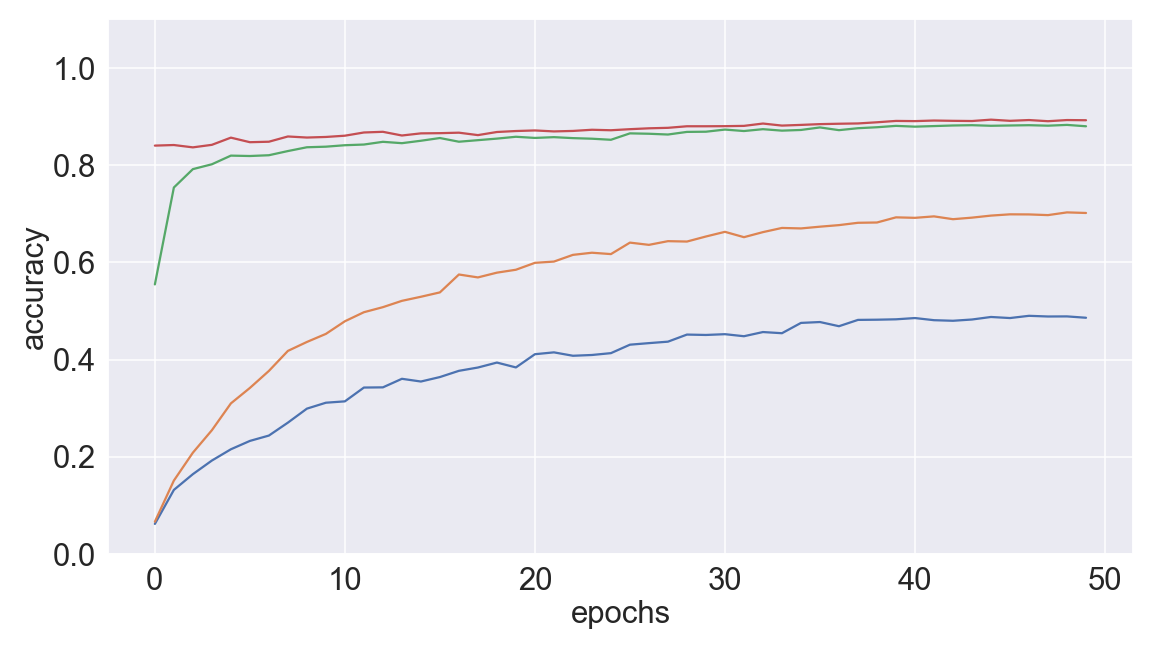
\includegraphics[width=.49\textwidth]{figures/training_plots/b-resnet_test-accuracy}}
	\caption[B-ResNet Training summary]{B-ResNet Training summary: shows the progression of model attributes over times of epochs, \protect\subref{fig:b-resnet-train-loss} train loss, \protect\subref{fig:b-resnet-test-loss} test loss, \protect\subref{fig:b-resnet-train-acc} train accuracy, \protect\subref{fig:b-resnet-test-acc}, test accuracy.}
	\label{fig:b-resnet-miniimagenet-100}
\end{figure}

Table \ref{tbl:frozen-vs-unfrozen}  shows the improvement of the higest validation score obtained in the training process. Comparing the two show, that we are able to improve the accuracy at early exits, thus the features located in the shallower part of the model now provides information that enables the classifiers to better discriminate the classes. 

\begin{longtabu}{>{\bfseries}X[2]|X[r]|X[r]|X[r]|X[r]}
	\caption[Comparison of Transfer Learning Approaches]{Comparison of transfer learning approaches frozen model vs. fine-tuning on validation accuracy} \label{tbl:frozen-vs-unfrozen} \\
	\toprule
	\rowfont{\bfseries}
	Model & Exit-0 & Exit-1 & Exit-2 & Exit-3 \tabularnewline
	\bottomrule
	\endfirsthead
	\multicolumn{3}{@{}l}{\textbf{\textcolor{black}{Table \ref{tbl:frozen-vs-unfrozen}:}} continued}\\
	\toprule
	\rowfont{\bfseries}
	Model & Exit-0 & Exit-1 & Exit-2 & Exit-1 \tabularnewline
	\bottomrule
	\endhead % all the lines above this will be repeated on every page
	\bottomrule
	\multicolumn{3}{@{}l}{continued \ldots}\\
	\endfoot
	\hline
	\endlastfoot
	Frozen B-\gls{resnet}	& 0.14	& 0.18	& 0.63 & 0.93 \tabularnewline
	\hline
	Unfrozen B-\gls{resnet}	& 0.49 	& 0.70 & 0.88 & 0.89 \tabularnewline
	\hline
	Gain & 3.50 & 3.89 & 1.40 &  0.96  \tabularnewline							
	\bottomrule
\end{longtabu}

As the two last exits of \gls{resnet} is almost equally accurate, not much gain is obtained by running the model all the way to the end. Figure \ref{fig:b-densenet-miniimagenet-100} show the training result of B-\gls{densenet}. B-\gls{densenet} on the other hand always have a gain in accuracy by continuing the inference process all the way to the end, and are also able to achieve better accuracy at earlier exits than B-\gls{resnet}. However, again at the cost of less accurate end exit. The figure shows the same importance of the densely connected layers for an early exit model as in \cite{huang_multi-scale_2017}. Eventhough the two first exits of \gls{bdensenet} have a higher accuracy, the last two exits obtain higher accuracy for the Figure \ref{fig:b-densenet-miniimagenet-100} show the training result of \gls{bdensenet}, see table \ref{tbl:training-compariosn}. \gls{msdnet}, the early exiting version of \gls{densenet}, shows further improvement to early exits accuracy.     

\begin{figure}
	\centering
	\captionsetup[subfigure]{justification=centering, farskip=1pt,captionskip=1pt}
	
\includegraphics[width=.5\textwidth]{figures/training_plots/b-densenet_exit_legend}
	\subfloat[Train loss\label{fig:b-densenet-train-loss}]{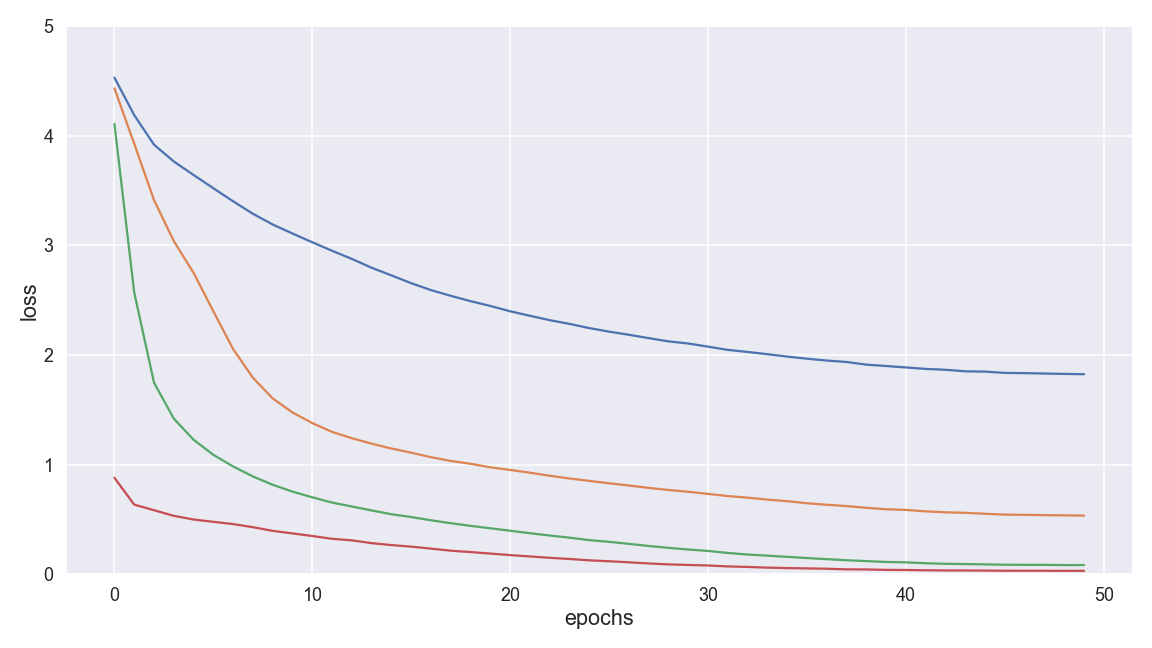
\includegraphics[width=.49\textwidth]{figures/training_plots/b-densenet_train-loss}}
	\subfloat[Test loss \label{fig:b-densenet-test-loss}]{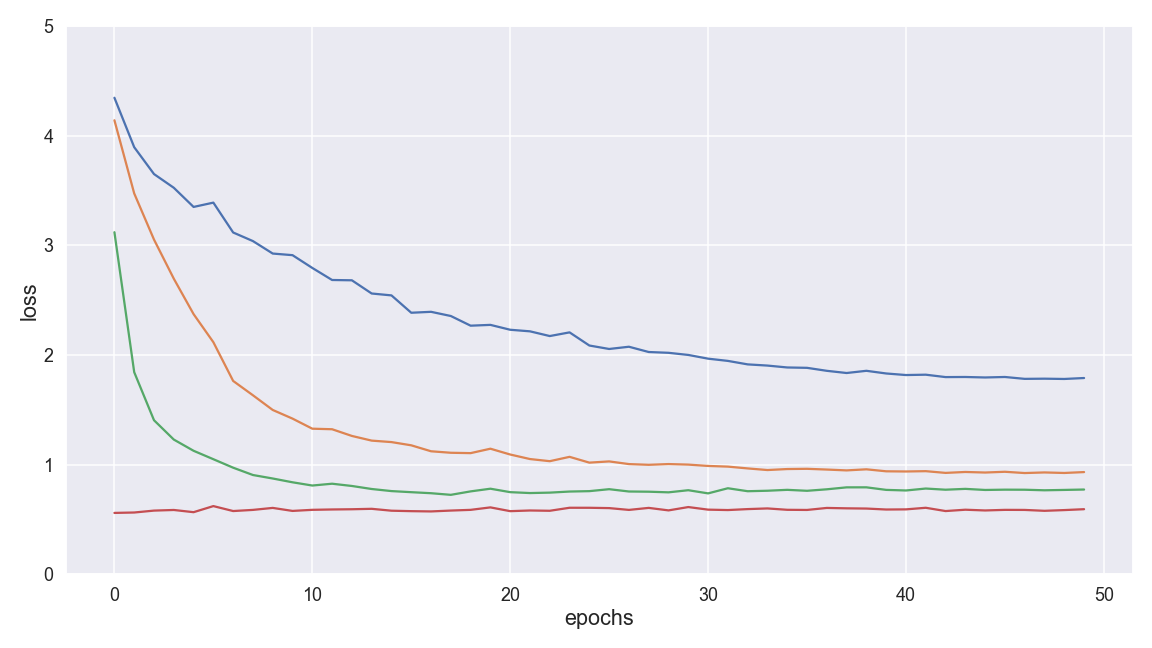
\includegraphics[width=.49\textwidth]{figures/training_plots/b-densenet_test-loss}}
	\hfill
	\subfloat[Train accuracy\label{fig:b-densenet-train-acc}]{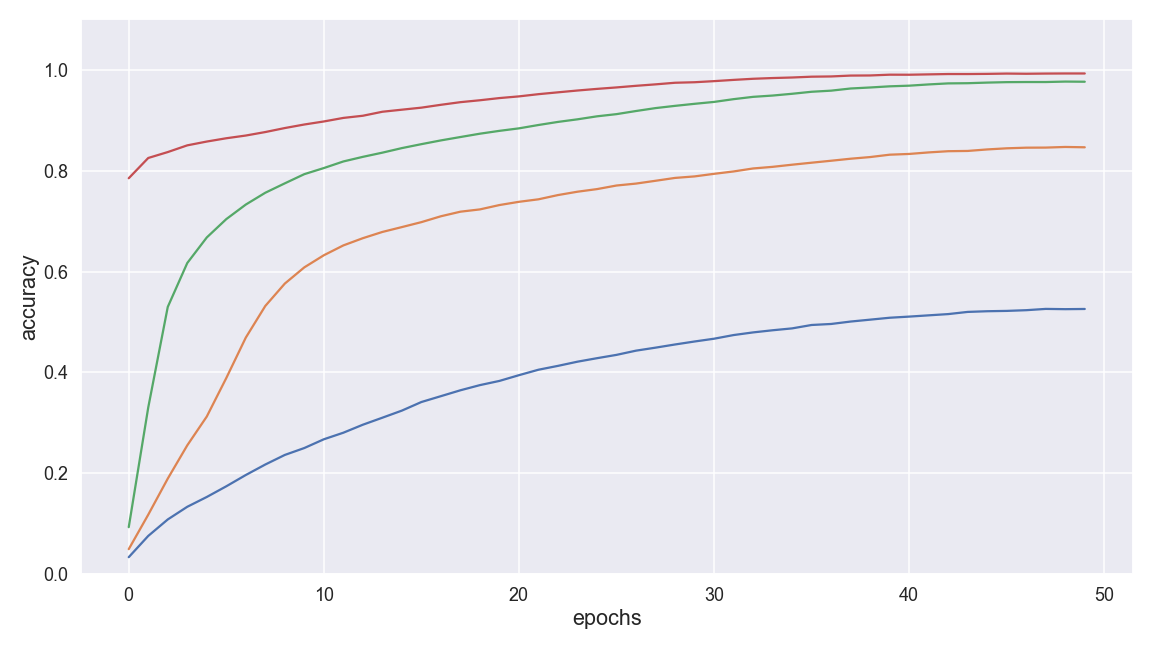
\includegraphics[width=.49\textwidth]{figures/training_plots/b-densenet_train-accuracy}}
	\subfloat[Test accuracy\label{fig:b-densenet-test-acc}]{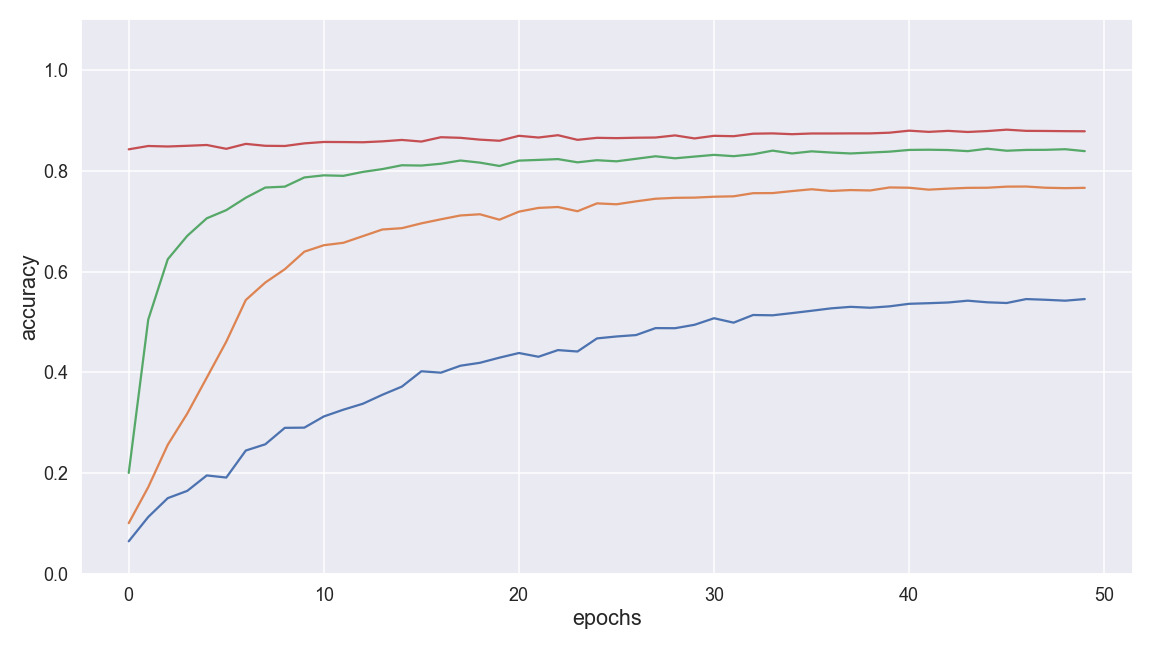
\includegraphics[width=.49\textwidth]{figures/training_plots/b-densenet_test-accuracy}}
	\caption[B-densenet Training summary]{B-densenet Training summary: shows the progression of model attributes over times of epochs, \protect\subref{fig:b-densenet-train-loss} train loss, \protect\subref{fig:b-densenet-test-loss} test loss, \protect\subref{fig:b-densenet-train-acc} train accuracy, \protect\subref{fig:b-densenet-test-acc}, test accuracy.}
	\label{fig:b-densenet-miniimagenet-100}
\end{figure}

Figure \ref{fig:msdnet-miniimagenet-100} show the results of training the \gls{msdnet}. The model specifically designed for early exiting shows indeed improvements for classifiers at early exit, but the overall accuracy i.e. the accuracy of the final classifier is slightly smaller compared to the other two models.

\begin{figure}
	\centering
	\captionsetup[subfigure]{justification=centering, farskip=1pt,captionskip=1pt}
	
\includegraphics[width=.5\textwidth]{figures/training_plots/msdnet_exit_legend}
	\subfloat[Train loss\label{fig:msdnet-train-loss}]{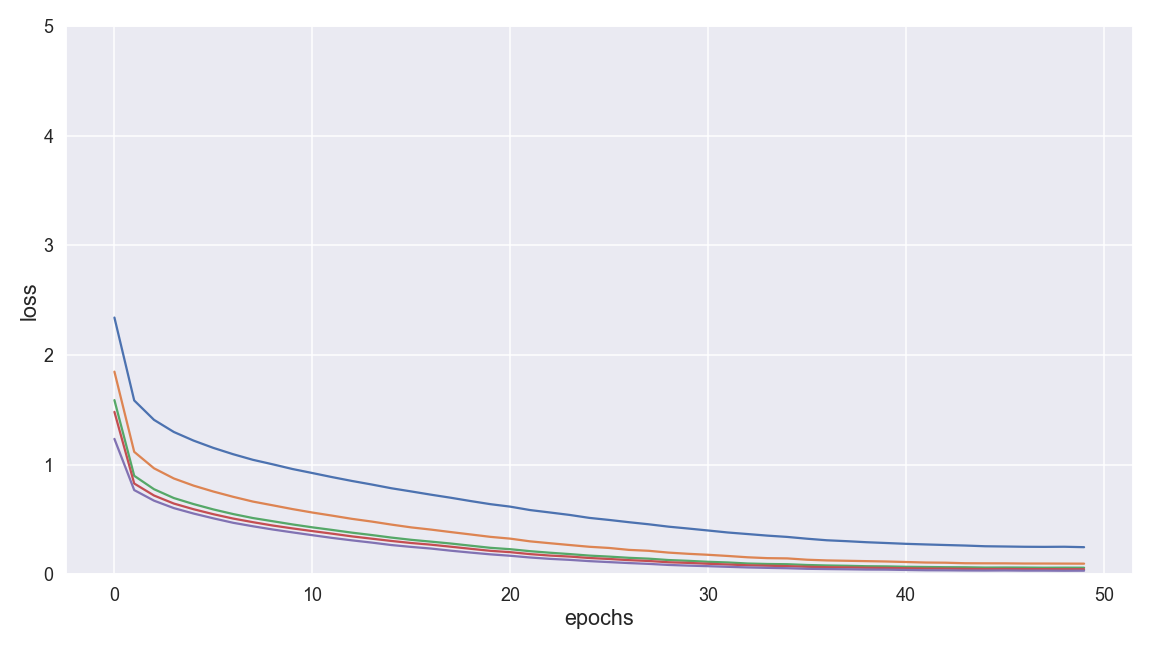
\includegraphics[width=.49\textwidth]{figures/training_plots/msdnet_train-loss}}
	\subfloat[Test loss \label{fig:msdnet-test-loss}]{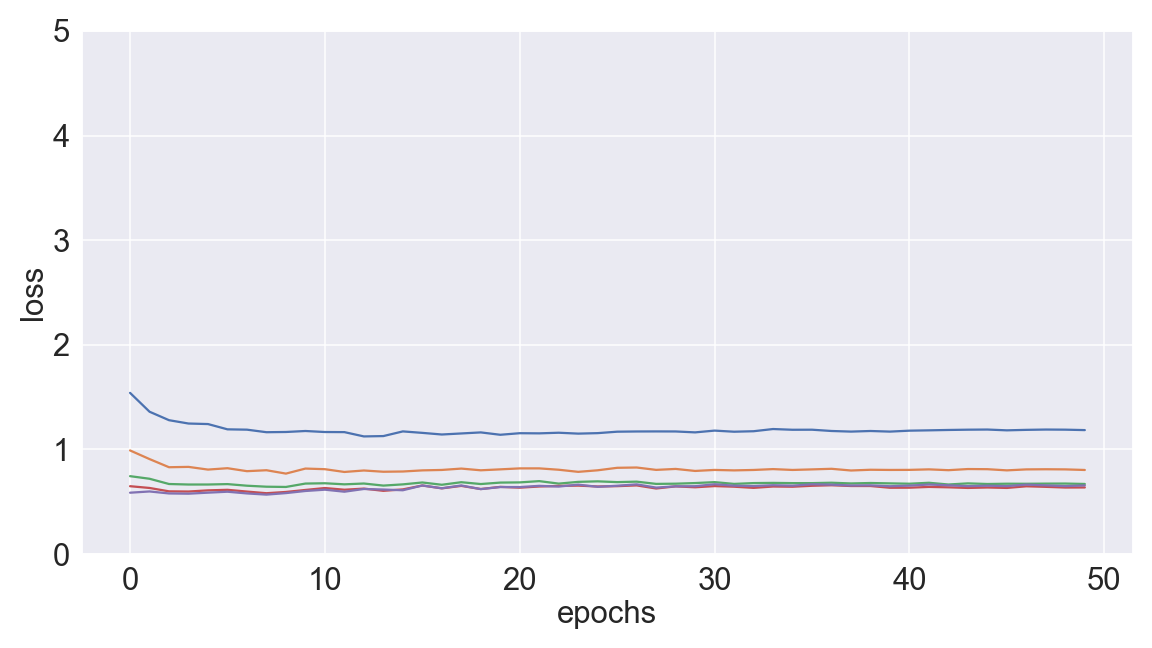
\includegraphics[width=.49\textwidth]{figures/training_plots/msdnet_test-loss}}
	\hfill
	\subfloat[Train accuracy\label{fig:msdnet-train-acc}]{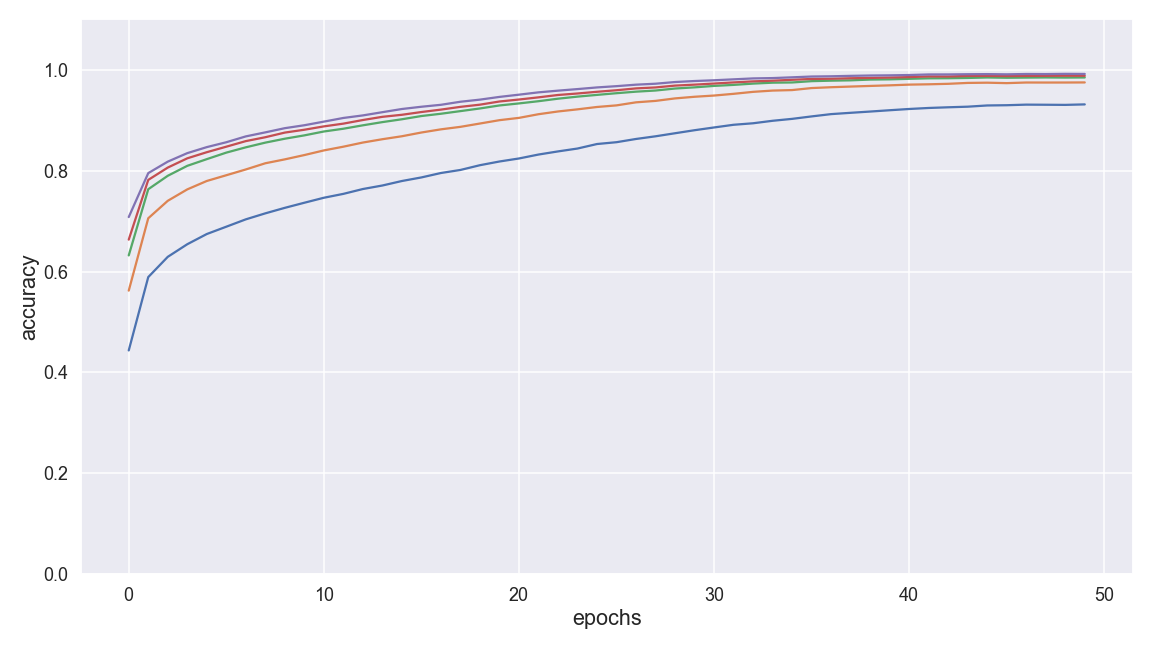
\includegraphics[width=.49\textwidth]{figures/training_plots/msdnet_train-accuracy}}
	\subfloat[Test accuracy\label{fig:msdnet-test-acc}]{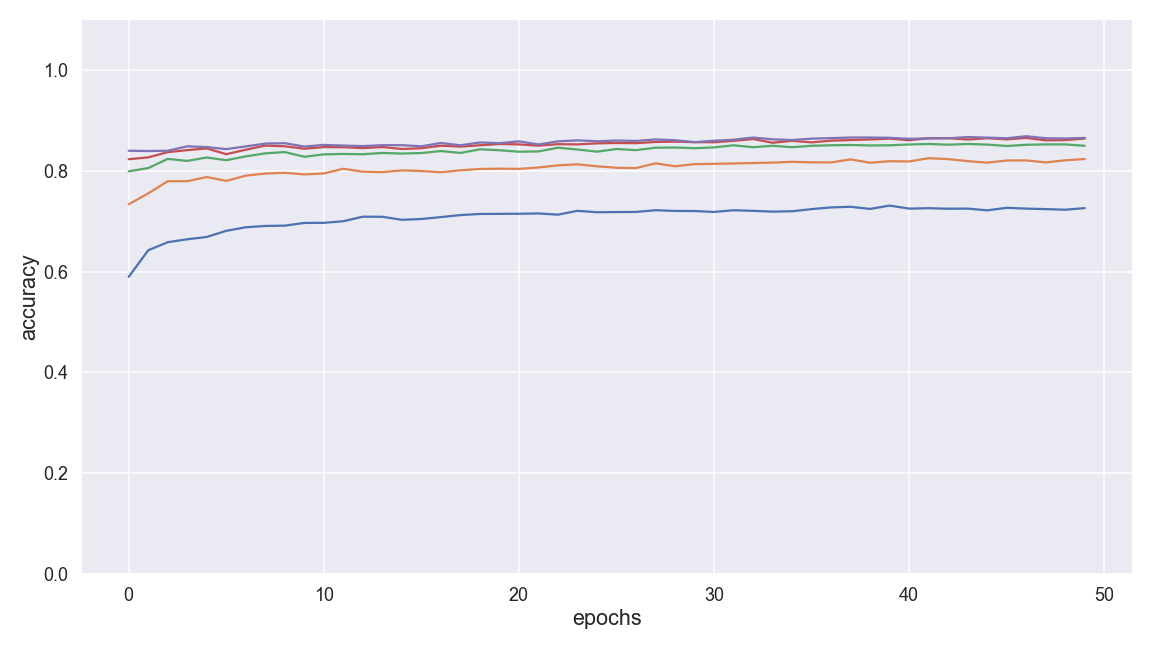
\includegraphics[width=.49\textwidth]{figures/training_plots/msdnet_test-accuracy}}
	\caption[MSDNet Training summary]{MSDNet Training summary: shows the progression of model attributes over times of epochs, \protect\subref{fig:msdnet-train-loss} train loss, \protect\subref{fig:msdnet-test-loss} test loss, \protect\subref{fig:msdnet-train-acc} train accuracy, \protect\subref{fig:msdnet-test-acc}, test accuracy.}
	\label{fig:msdnet-miniimagenet-100}
\end{figure}

Table \ref{tbl:training-compariosn} compares the best obtained validation accuracy in the training processes of the three models.


\begin{longtabu}{>{\bfseries}X[2]|X|X|X|X|X}
	\caption[Early Exiting Validation Accuracy from Training]{Early Exiting Validation Accuracy from Training} \label{tbl:training-compariosn} \\
	\toprule
	\rowfont{\bfseries}
	Model & Exit-0 & Exit-1 & Exit-2 & Exit-3 & Exit-4 \tabularnewline
	\bottomrule
	\endfirsthead
	\multicolumn{3}{@{}l}{\textbf{\textcolor{black}{Table \ref{tbl:frozen-vs-unfrozen}:}} continued}\\
	\toprule
	\rowfont{\bfseries}
	Model & Exit-0 & Exit-1 & Exit-2 & Exit-3 & Exit-4 \tabularnewline
	\bottomrule
	\endhead % all the lines above this will be repeated on every page
	\bottomrule
	\multicolumn{3}{@{}l}{continued \ldots}\\
	\endfoot
	\hline
	\endlastfoot
	B-\gls{resnet} & 0.49 	& 0.70 & 0.88 & 0.89 & N/A \tabularnewline
	\hline
	B-\gls{densenet}	& 0.55 	& 0.77 & 0.84 & 0.88 & N/A \tabularnewline
	\hline
	\gls{msdnet} & 0.73 & 0.82 & 0.85 &  0.87 & 0.87 \tabularnewline							
	\bottomrule
\end{longtabu}

In the next section we evaluate the trained models on the \gls{min100} validation set.

\subsection{Inference Results}

In this section we evaluate the accuracy of the early exit models. All validation samples are inferred to all model of table \ref{tbl:models}. Figure \ref{fig:exit-accuracy} show top-1 and top-5 accuracy of all exits of the three models.  

\begin{figure}
	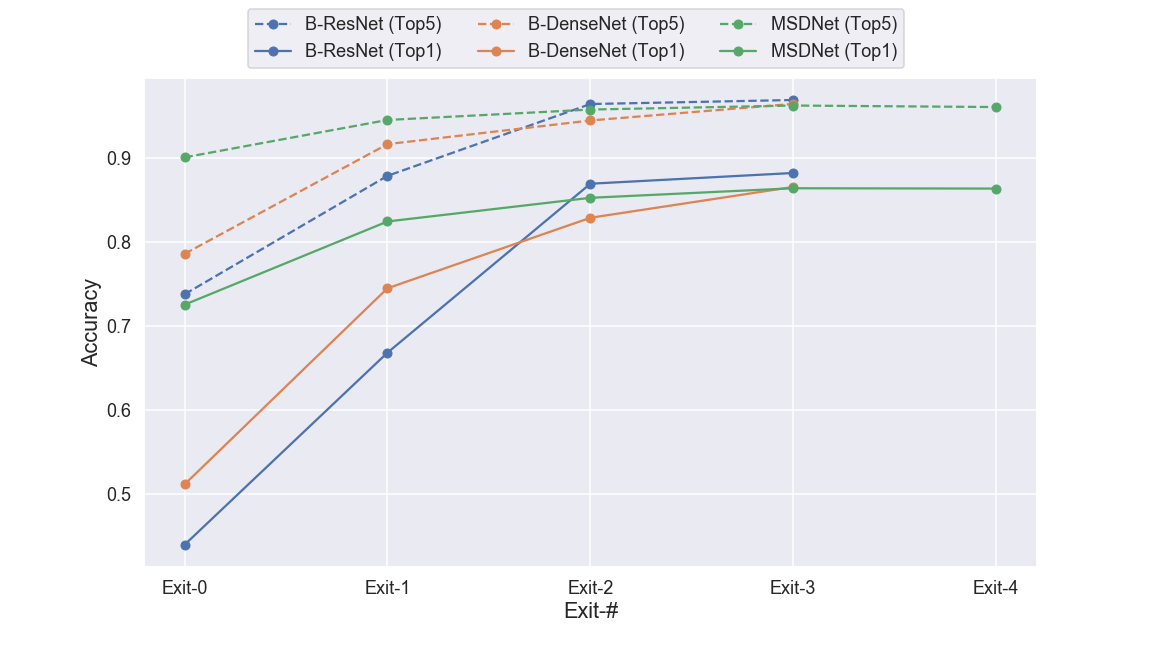
\includegraphics[width=\linewidth]{figures/inference_plots/accuracy-comparison}
	\caption[Accuracy of Early Exit Models]{Accuracy of Early Exit Models, B-\gls{resnet}, B-\gls{densenet} and \gls{msdnet}}
	\label{fig:exit-accuracy}
\end{figure}

As expected the models become more accurate, as the samples are predicted deeper in the network, as the increasingly complex features deep within the network have more discriminative characteristics. As stated in \cite{huang_multi-scale_2017} the densely connected features are important factors for obtaining intermediate classifiers with decent accuracy. The \gls{bdensenet} and \gls{msdnet} have as expected more accurate early classifiers, however the end-exit of \gls{bresnet} achieves superior top-1 accuracy compared to the other models. Close to 50 \% of the samples can be accurately classified at the first exit of any of the model, which justifies the assumption for early exiting and promisingly, we should be able to save time. 

\subsubsection{Inference Time Analysis}

We setup a test, where we inference the entire \gls{min100} validation set the in all 5 models on three different platforms. Table \ref{tbl:inference-stats} show statistical values mean, standard deviation, minimum and maximum for the model inference time on the different platforms. From the table one can see, that the early exiting framework adds only a small additional delay, when comparing the last exit the \gls{branchynet} version with its conventional pendant. For the \gls{gpu}-enabled platforms, \gls{gpu} Workstation Jetson TX2, only additional 1.1ms and 2.4ms respectively on average. On the NUC the \gls{bresnet} is 7.5 ms slower. 
\small{
\begin{longtabu}{>{\bfseries}X[2.6]|[1pt]X[r]|X[0.8r]|X[r]|X[1.2r]|[1pt]X[r]|X[0.7r]|X[r]|X[1.2r]|[1pt]X[r]|X[0.7r]|X[r]|X[1.2r]}
	\caption[Inference time statistics]{Inference time statistics (mean, standard deviation, minimum, maximum) of the five models on the three platforms }\label{tbl:inference-stats} \\
	\toprule
	\rowfont{\bfseries}
	& \multicolumn4{c|[1pt]}{GPU Workstation} &  \multicolumn4{c|[1pt]}{Jetson TX2} & \multicolumn4{c}{Intel NUC} \tabularnewline
	\tabucline{2-13}
	\rowfont{\bfseries} Model & Mean & Std.  & Min & Max & Mean & Std. & Min & Max & Mean & Std.  & Min & Max  \tabularnewline
	\hline
	\endfirsthead
	\multicolumn{3}{@{}l}{\textbf{\textcolor{black}{Table \ref{tbl:inference-stats}:}} continued}\\
	\toprule
	\rowfont{\bfseries}
	& \multicolumn4{c|[1pt]}{GPU Workstation} &  \multicolumn4{c|[1pt]}{Jetson TX2} & \multicolumn4{c}{Intel NUC} \tabularnewline
	\tabucline{2-13}
	\rowfont{\bfseries} Model & Mean & Std.  & Min & Max & Mean & Std.  & Min & Max & Mean & Std.  & Min & Max  \tabularnewline
	\hline
	\endhead % all the lines above this will be repeated on every page
	\hline
	\multicolumn{3}{@{}l}{continued \ldots}\\
	\endfoot
	\hline
	\endlastfoot
	ResNet  	& 36.01 & 1.72 & 33.24 & 69.02 & 64.19 & 1.95 & 61.28 & 110.17 & 215.76 & 21.98 & 132.98 & 275.55 \tabularnewline
	\hline
	DenseNet 	& 47.74 & 1.95 & 4.48 & 86.88 & 70.48 & 3.04 & 59.56 & 132.45 &  72.30 &  2.61 &  69.02 & 107.63 \tabularnewline
	\hline
	B-ResNet & & & &&&&&&&& &  \tabularnewline 
	\hspace{3mm} Exit-0 &  4.20 & 0.63 &  3.81 &  39.40 &  8.61 & 0.31 &  8.39 &  15.54 &  38.25 &  1.85 &  29.26 &  74.94 \tabularnewline
	\hspace{3mm} Exit-1 &  9.40 & 1.28 &  8.19 &  70.23 & 19.30 & 1.08 & 16.42 &  38.41 &  66.69 &  3.15 &  50.41 & 110.80 \tabularnewline
	\hspace{3mm} Exit-2 & 33.59 & 2.78 & 30.25 & 103.55 & 56.77 & 2.73 & 52.34 & 102.58 & 196.43 &  8.81 & 150.11 & 254.86 \tabularnewline
	\hspace{3mm} Exit-3 & 37.14 & 2.94 & 33.65 & 109.94 & 67.04 & 2.86 & 62.47 & 116.74 & 223.32 & 10.35 & 170.95 & 289.67 \tabularnewline
	\hline
	B-DenseNet &  & & &&&&&&&& & \tabularnewline
	\hspace{3mm} Exit-0 &  5.83 & 1.09 &  5.15 &  54.61 & 11.05 & 0.48 & 10.52 & 17.31 &  28.83 & 1.59 & 26.05 & 41.93 \tabularnewline
	\hspace{3mm} Exit-1 & 17.03 & 1.89 & 14.60 &  76.78 & 30.26 & 2.02 & 23.75 & 47.54 &  46.71 & 2.31 & 43.47 & 71.85 \tabularnewline
	\hspace{3mm} Exit-2 & 36.31 & 3.01 & 32.72 & 104.79 & 55.38 & 3.22 & 48.10 & 87.81 &  64.26 & 2.80 & 60.65 & 99.41 \tabularnewline
	\hspace{3mm} Exit-3 & 49.14 & 3.36 & 45.13 & 127.07 & 72.41 & 3.89 & 64.77 & 120.29 & 72.21 & 2.97 & 68.37 & 112.06 \tabularnewline
	\hline
	MSDNet & & &&&&&&&&&& \tabularnewline
	\hspace{3mm} Exit-0 & 24.14 & 1.59 & 21.53 &  67.38 &  40.37 & 2.77 & 29.36 & 209.89 & 19.99 & 1.27 & 16.99 &  35.12 \tabularnewline
	\hspace{3mm} Exit-1 & 42.24 & 2.54 & 38.87 & 119.85 &  65.18 & 4.29 & 53.34 & 267.19 & 32.82 & 2.38 & 29.03 & 103.19 \tabularnewline
	\hspace{3mm} Exit-2 & 55.59 & 2.82 & 51.90 & 143.30 &  83.81 & 5.43 & 71.39 & 312.55 & 42.89 & 3.03 & 38.72 & 130.52 \tabularnewline
	\hspace{3mm} Exit-3 & 64.49 & 2.99 & 60.59 & 156.26 &  96.53 & 6.26 & 83.68 & 345.67 & 50.10 & 3.43 & 45.66 & 145.75 \tabularnewline
	\hspace{3mm} Exit-4 & 68.87 & 3.11 & 64.85 & 165.90 & 103.29 & 6.65 & 90.14 & 361.02 & 56.02 & 3.62 & 51.28 & 154.08 \tabularnewline
	\bottomrule
\end{longtabu}}
\normalsize

Figure \ref{fig:inference-time-dist} shows the inference timing results as histograms. The inference time for each exit are plotted. The inference time are very different on the three platforms, and is very much dependent on the hardware characteristics, this is elaborated upon in section \ref{sec:ee-summary}.

\begin{figure}
	\begin{minipage}{\textwidth}
		\centering
		
\includegraphics[width=.5\linewidth]{figures/inference_plots/time_dist_legend}
	\end{minipage}
	\begin{minipage}{0.33\textwidth}
		\captionsetup[subfigure]{farskip=0pt,captionskip=0pt, justification=centering}
		\centering
		GPU Workstation
		\subfloat[\gls{resnet} ]{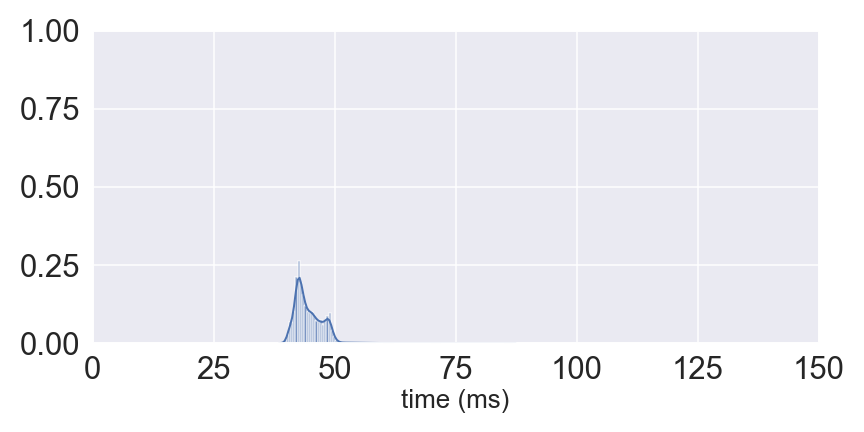
\includegraphics[width=\textwidth,height=.2\textheight,keepaspectratio]{figures/inference_plots/gpu_resnet_inference_time_distribution}}
		\hfill
		\subfloat[B-\gls{resnet}]{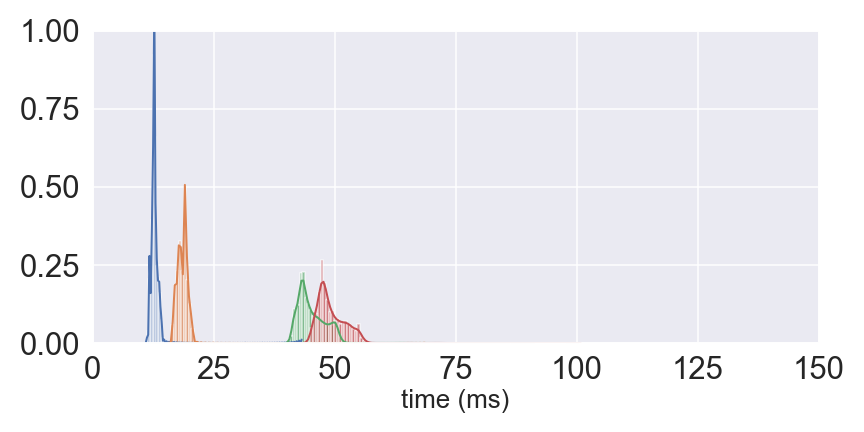
\includegraphics[width=\textwidth,height=.2\textheight,keepaspectratio]{figures/inference_plots/gpu_b-resnet_inference_time_distribution}}
		\hfill
		\subfloat[\gls{densenet} ]{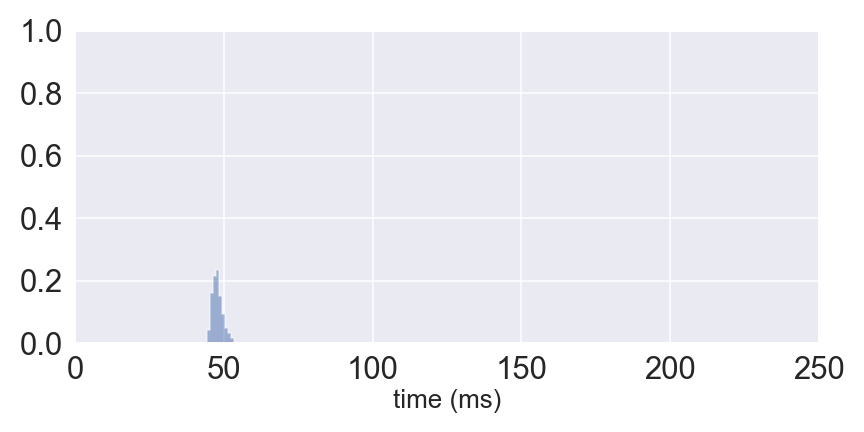
\includegraphics[width=\textwidth,height=.2\textheight,keepaspectratio]{figures/inference_plots/gpu_densenet_inference_time_distribution}}
		\hfill
		\subfloat[B-\gls{densenet}]{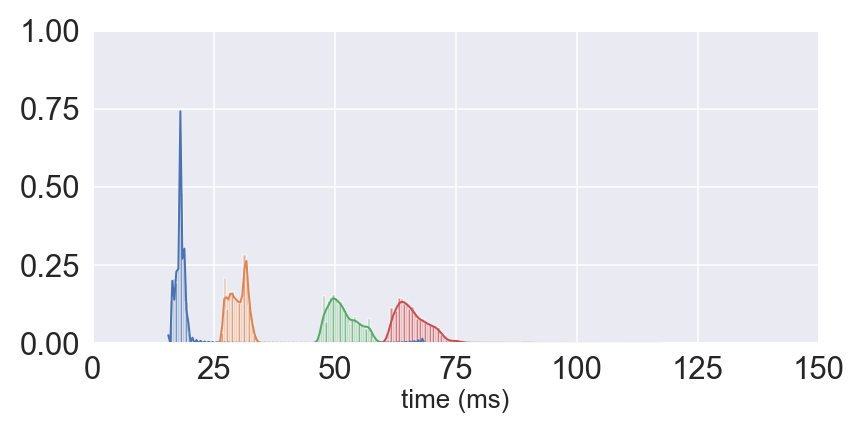
\includegraphics[width=\textwidth,height=.2\textheight,keepaspectratio]{figures/inference_plots/gpu_b-densenet_inference_time_distribution}}
		\hfill
		\subfloat[\gls{msdnet}]{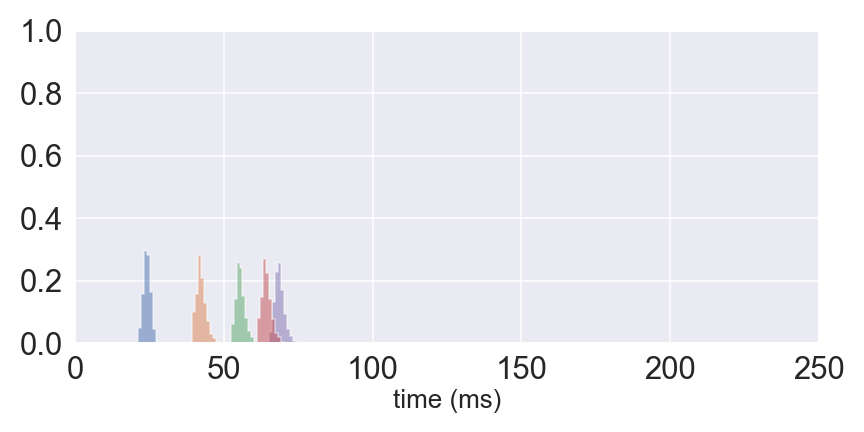
\includegraphics[width=\textwidth,height=.2\textheight,keepaspectratio]{figures/inference_plots/gpu_msdnet_inference_time_distribution}}
	\end{minipage}
	\begin{minipage}{0.33\textwidth}
		\captionsetup[subfigure]{farskip=0pt,captionskip=0pt,justification=centering}
		\centering
		Jetson TX2
		\subfloat[\gls{resnet} ]{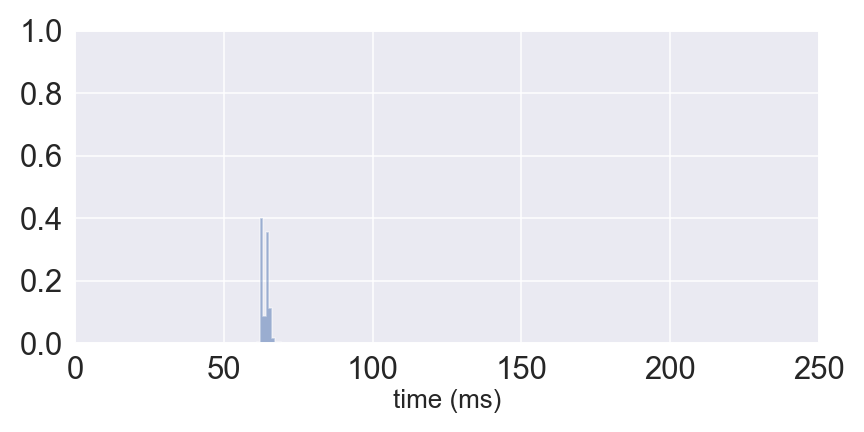
\includegraphics[width=\textwidth,height=.2\textheight,keepaspectratio]{figures/inference_plots/jetson_resnet_inference_time_distribution}}
		\hfill
		\subfloat[B-\gls{resnet}]{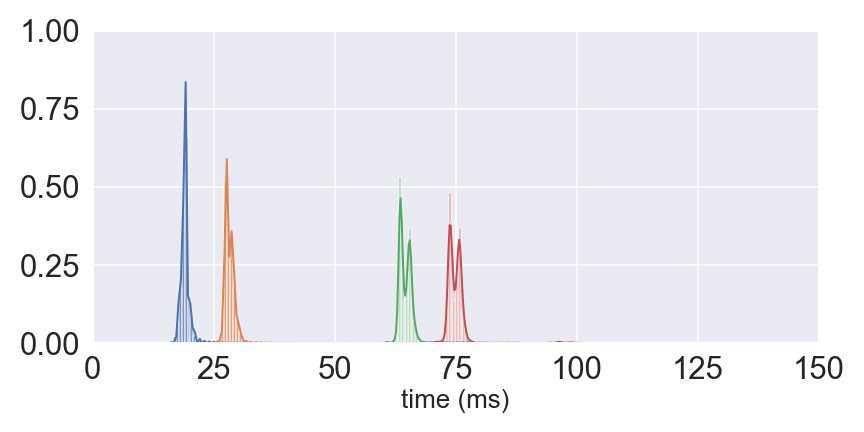
\includegraphics[width=\textwidth,height=.29\textheight,keepaspectratio]{figures/inference_plots/jetson_b-resnet_inference_time_distribution}}
		\hfill
		\subfloat[\gls{densenet} ]{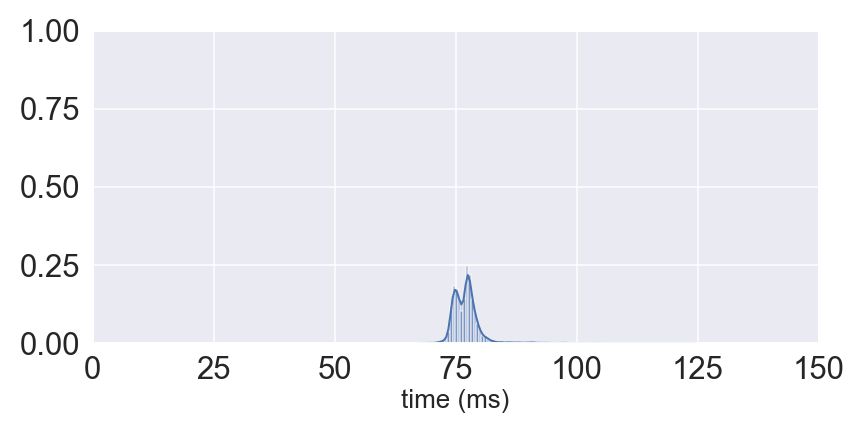
\includegraphics[width=\textwidth,height=.2\textheight,keepaspectratio]{figures/inference_plots/jetson_densenet_inference_time_distribution}}
		\hfill
		\subfloat[B-\gls{densenet}]{\includegraphics[width=\textwidth,height=.2\textheight,keepaspectratio]{figures/inference_plots/jetson_b-densenet_inference_time_distribution}}
		\hfill
		\subfloat[\gls{msdnet}]{\includegraphics[width=\textwidth,height=.2\textheight,keepaspectratio]{figures/inference_plots/jetson_msdnet_inference_time_distribution}}
	\end{minipage}
	\begin{minipage}{.33\textwidth}
		\captionsetup[subfigure]{farskip=0pt,captionskip=0pt,justification=centering}
		\centering
		Intel NUC
		\subfloat[\gls{resnet} ]{\includegraphics[width=\textwidth,keepaspectratio]{figures/inference_plots/nuc_resnet_inference_time_distribution}}
		\hfill
		\subfloat[B-\gls{resnet}]{\includegraphics[width=\textwidth,height=.2\textheight,keepaspectratio]{figures/inference_plots/nuc_b-resnet_inference_time_distribution}}
		\hfill
		\subfloat[\gls{densenet} ]{\includegraphics[width=\textwidth,keepaspectratio]{figures/inference_plots/nuc_densenet_inference_time_distribution}}
		\hfill
		\subfloat[B-\gls{densenet}]{\includegraphics[width=\textwidth,keepaspectratio]{figures/inference_plots/nuc_b-densenet_inference_time_distribution}}
		\hfill
		\subfloat[\gls{msdnet}]{\includegraphics[width=\textwidth,keepaspectratio]{figures/inference_plots/nuc_msdnet_inference_time_distribution}}	
	\end{minipage}
	\caption[Platform Inference Time of \gls{dnn}s]{Inference Time Distribution, left column: GPU Workstation (a-e), center column: Jetson TX2 (f-j), right column NUC (k-o)}
	\label{fig:inference-time-dist}
\end{figure}

Still the challenge remains, how to determine when to let samples exit? As mentionend in section \ref{sec:ee-branchy-vs-cascaded}, it has been done in literature using a threshold measure of confidence \cite{leroux_cascading_2017, teerapittayanon_branchynet:_2016}. In the next section, we investigate how to allow samples to exit the model prematurely using the output from the softmax classfier. We experiment with our two different score function: score-max and score-margin.

\subsubsection{Confidence Threshold Analysis}

Selecting threshold is a vital hyper-parameter for the accuracy-latency trade-off of early exiting models. If a too high threshold is selected only a few samples can confidently exit the model at an early exit, thus no significant delay improvements may be found. Contrary if too low a threshold is selected a huge delay improvement may be found, however at the cost of overall model accuracy. 

This analysis is theoretical, as the early exiting mechanism is in fact not exploited. All samples are allowed to pass all the way to the end of the network, thus all samples are classified at each exit, where both the prediction and score is logged. The prediction is evaluated against the ground truth and the score the two different score threshold measures, \emph{Score-max} and \emph{Score-Margin}. If the score is higher than the threshold, the samples is marked as exited. \Cref{fig:resnet_confidence,fig:resnet_score-margin,fig:densenet_confidence,fig:densenet_score-margin,fig:msdnet_confidence,fig:msdnet_score-margin} compares the performance of each exit on all samples. The figures show for each of the early exit models under test. We plot the two thresholds score metrics for all exit of the models. The figures shows the frequency of exited samples, that have been correctly classified ({\color{sns-green}green}), and incorrectly classified samples, that the model have exited due to satisfying score ({\color{sns-red}red}). The samples, that could not be exited with proper confidence score given the magnitude of the threshold ({\color{sns-blue}blue}). The line plotted on each subfigure, shows the change in accuracy for the exit, as we raise the confidence score requirements ({\color{sns-orange}orange}).  

The aim is to find the metric, that reduces the amount of incorrectly exited samples ({\color{sns-red}red}). Whenever samples are exited incorrectly, the overall accuracy of the models are reduced, if it could have been correctly classifed at later exit. The growing frequency of correctly exited samples ({\color{sns-green}green}) at later exits, exemplifies exactly this improved accuracy at deeper layers of the models. As the value of the threshold are raised, it results in a higher accuracy for the exit, as the number incorrectly exited grows faster, than the number of correctly exited samples. 

Generally \emph{score-margin} has more desirable traits, as less samples are incorrectly exited ({\color{sns-red}red}), at the expense of additional samples not exited ({\color{sns-blue}blue}). \emph{Score-margin} is thus slower, but also more accurate, as fewer samples are incorrectly exited. The results matches \cite{park_big/little_2015}, which shows a stronger correlation between \emph{score-margin} and accuracy, than confidence score and accuracy.

We comparing the three models, we can see the impact of densely connected layer of \gls{bdensenet} and \gls{msdnet}, that are able to obtain higher scores at early exits, thus accurately exiting more samples prematurely. \gls{bresnet} on the other hand are able to achieve higher end accuracy.

The theoretical analysis is followed up by a practical test, where samples are exited if the threshold is passed. The test evaluates the threshold impact on accuracy and latency. 

\newcounter{imagenumber}
\begin{minipage}{\textwidth}
	\begin{figure}
		\centering
		\paragraph{B-ResNet}
		\includegraphics[width=\linewidth]{figures/threshold_plots/threshold_analysis_legend}
	\end{figure}
	
	\begin{minipage}{0.5\textwidth}
		\begin{figure}
			\captionsetup[subfloat]{farskip=1pt,captionskip=1pt, justification=centering}
			\centering
			\forloop{imagenumber}{0}{\value{imagenumber} < 4}{
				
				\subfloat[Exit-\arabic{imagenumber}\label{fig:confidence_resnet_exit_\arabic{imagenumber}}]{\includegraphics[width=.9\linewidth]{figures/threshold_plots/threshold_analysis_b-resnet_confidence_\arabic{imagenumber}}}
				\hfill
			}
			\caption[ResNet Confidence Threshold]{Confidence Threshold}
			\label{fig:resnet_confidence}
		\end{figure}
	\end{minipage}
	\begin{minipage}{0.5\textwidth}
		\begin{figure}
			\captionsetup[subfloat]{farskip=1pt,captionskip=1pt, justification=centering}
			\centering
			\forloop{imagenumber}{0}{\value{imagenumber} < 4}{
				
				\subfloat[Exit-\arabic{imagenumber}\label{fig:score-margin_resnet_exit_\arabic{imagenumber}}]{\includegraphics[width=.9\linewidth]{figures/threshold_plots/threshold_analysis_b-resnet_score-margin_\arabic{imagenumber}}}
				\hfill
			}
			\caption[ResNet Score-margin Threshold]{Score-margin Threshold}
			\label{fig:resnet_score-margin}
		\end{figure}
	\end{minipage}
\end{minipage}

\begin{minipage}{\textwidth}
	\begin{figure}
		\centering
		\paragraph{B-DenseNet}
	\end{figure}
	\begin{minipage}{0.5\textwidth}
		\begin{figure}
			\captionsetup[subfloat]{farskip=1pt,captionskip=1pt, justification=centering}
			\centering
			\forloop{imagenumber}{0}{\value{imagenumber} < 4}{
				
				\subfloat[Exit-\arabic{imagenumber}\label{fig:confidence_dense_exit_\arabic{imagenumber}}]{\includegraphics[width=.9\linewidth]{figures/threshold_plots/threshold_analysis_b-densenet_confidence_\arabic{imagenumber}}}
				\hfill
			}
			\caption[DenseNet Confidence Threshold]{Confidence Threshold}
			\label{fig:densenet_confidence}
		\end{figure}
	\end{minipage}
	\begin{minipage}{0.5\textwidth}
		\begin{figure}
			\captionsetup[subfloat]{farskip=1pt,captionskip=1pt, justification=centering}
			\centering
			\forloop{imagenumber}{0}{\value{imagenumber} < 4}{
				
				\subfloat[Exit-\arabic{imagenumber}\label{fig:score-dense_resnet_exit_\arabic{imagenumber}}]{\includegraphics[width=.9\linewidth]{figures/threshold_plots/threshold_analysis_b-densenet_score-margin_\arabic{imagenumber}}}
				\hfill
			}
			\caption[DenseNet Score-margin Threshold]{Score-margin Threshold}
			\label{fig:densenet_score-margin}
		\end{figure}
	\end{minipage}
\end{minipage}

\noindent\makebox[\textwidth][c]{\begin{minipage}{0.9\textwidth}
		\begingroup
		\leftskip=0cm plus 0.5fil \rightskip=0cm plus -0.5fil
		\parfillskip=0cm plus 1fil
		\paragraph{MSDNet}\par
		\endgroup
		
		\begin{minipage}{0.5\textwidth}
			\begin{figure}
				\captionsetup[subfloat]{farskip=0pt,captionskip=0pt, justification=centering}
				\centering
				\forloop{imagenumber}{0}{\value{imagenumber} < 5}{
					
					\subfloat[Exit-\arabic{imagenumber}\label{fig:confidence_msd_exit_\arabic{imagenumber}}]{\includegraphics[width=.9\linewidth]{figures/threshold_plots/threshold_analysis_msdnet_confidence_\arabic{imagenumber}}}
					\hfill
				}
				\caption[MSDNet Confidence Threshold]{Confidence Threshold}
				\label{fig:msdnet_confidence}
			\end{figure}
		\end{minipage}
		\begin{minipage}{0.5\textwidth}
			\begin{figure}
				\captionsetup[subfloat]{farskip=1pt,captionskip=1pt, justification=centering}
				\centering
				\forloop{imagenumber}{0}{\value{imagenumber} < 5}{
					
					\subfloat[Exit-\arabic{imagenumber}\label{fig:score-msdnet_exit_\arabic{imagenumber}}]{\includegraphics[width=.9\linewidth]{figures/threshold_plots/threshold_analysis_msdnet_score-margin_\arabic{imagenumber}}}
					\hfill
				}
				\caption[MSDNet Score-margin Threshold]{Score-margin Threshold}
				\label{fig:msdnet_score-margin}
			\end{figure}
		\end{minipage}
\end{minipage}}

\subsubsection{Practical Threshold Exiting}

We setup a test, where we use our three models, \gls{bresnet}, \gls{bdensenet} and \gls{msdnet}. In this test a sample is exited when a threshold is passed, thus no additional prediction are tried for the sample, to evaluate early exiting capabilities in practice. If a samples reaches the last exit, it is classified irregardless of threshold being passed or not. Figure \ref{fig:model_c-threshold_comparison} presents the result using the score-max and figure \ref{fig:model_threshold_comparison} using the score-margin.

\begin{minipage}{\linewidth}
	\begin{figure}
		\captionsetup[subfloat]{justification=centering, captionskip=0pt, farskip=0pt}
		\centering
		\includegraphics[width=.5\linewidth]{figures/inference_plots/model_bar_legend}
	\end{figure}
	\begin{figure}
		\captionsetup[subfloat]{justification=centering, captionskip=0pt, farskip=1pt}
		\centering
		\subfloat[$T= 0.1$\label{fig:model-c-threshold_comparison_t_1}]{\includegraphics[width=.33\linewidth]{figures/inference_plots/model_confidence_comparison_1}}
		\hfill
		\subfloat[$T= 0.2$\label{fig:model-c-threshold_comparison_t_2}]{\includegraphics[width=.33\linewidth]{figures/inference_plots/model_confidence_comparison_2}}
		\hfill
		\subfloat[$T= 0.3$\label{fig:model-c-threshold_comparison_t_3}]{\includegraphics[width=.33\linewidth]{figures/inference_plots/model_confidence_comparison_3}}
		\hfill
		\subfloat[$T= 0.4$\label{fig:model-c-threshold_comparison_t_4}]{\includegraphics[width=.33\linewidth]{figures/inference_plots/model_confidence_comparison_4}}
		\hfill
		\subfloat[$T= 0.5$\label{fig:model-c-threshold_comparison_t_5}]{\includegraphics[width=.33\linewidth]{figures/inference_plots/model_confidence_comparison_5}}
		\hfill
		\subfloat[$T= 0.6$\label{fig:model-c-threshold_comparison_t_6}]{\includegraphics[width=.33\linewidth]{figures/inference_plots/model_confidence_comparison_6}}
		\hfill
		\subfloat[$T= 0.7$\label{fig:model-c-threshold_comparison_t_7}]{\includegraphics[width=.33\linewidth]{figures/inference_plots/model_confidence_comparison_7}}
		\hfill
		\subfloat[$T= 0.8$\label{fig:model-c-threshold_comparison_t_8}]{\includegraphics[width=.33\linewidth]{figures/inference_plots/model_confidence_comparison_8}}
		\hfill
		\subfloat[$T= 0.9$\label{fig:model-c-threshold_comparison_t_9}]{\includegraphics[width=.33\linewidth]{figures/inference_plots/model_confidence_comparison_9}}
		
		\caption[Model comparison of early exit capabilities using confidence threshold]{Model comparison of early exit capabilities using score-max}
		\label{fig:model_c-threshold_comparison}
	\end{figure}
	
\end{minipage}

\begin{minipage}{\linewidth}
	\begin{figure}
		\captionsetup[subfloat]{justification=centering, captionskip=0pt, farskip=0pt}
		\centering
		\includegraphics[width=.5\linewidth]{figures/inference_plots/model_bar_legend}
	\end{figure}
	\begin{figure}
		\captionsetup[subfloat]{justification=centering, captionskip=0pt, farskip=1pt}
		\centering
		\subfloat[$T= 0.1$\label{fig:model-threshold_comparison_t_1}]{\includegraphics[width=.33\linewidth]{figures/inference_plots/model_comparison_1}}
		\hfill
		\subfloat[$T= 0.2$\label{fig:model-threshold_comparison_t_2}]{\includegraphics[width=.33\linewidth]{figures/inference_plots/model_comparison_2}}
		\hfill
		\subfloat[$T= 0.3$\label{fig:model-threshold_comparison_t_3}]{\includegraphics[width=.33\linewidth]{figures/inference_plots/model_comparison_3}}
		\hfill
		\subfloat[$T= 0.4$\label{fig:model-threshold_comparison_t_4}]{\includegraphics[width=.33\linewidth]{figures/inference_plots/model_comparison_4}}
		\hfill
		\subfloat[$T= 0.5$\label{fig:model-threshold_comparison_t_5}]{\includegraphics[width=.33\linewidth]{figures/inference_plots/model_comparison_5}}
		\hfill
		\subfloat[$T= 0.6$\label{fig:model-threshold_comparison_t_6}]{\includegraphics[width=.33\linewidth]{figures/inference_plots/model_comparison_6}}
		\hfill
		\subfloat[$T= 0.7$\label{fig:model-threshold_comparison_t_7}]{\includegraphics[width=.33\linewidth]{figures/inference_plots/model_comparison_7}}
		\hfill
		\subfloat[$T= 0.8$\label{fig:model-threshold_comparison_t_8}]{\includegraphics[width=.33\linewidth]{figures/inference_plots/model_comparison_8}}
		\hfill
		\subfloat[$T= 0.9$\label{fig:model-threshold_comparison_t_9}]{\includegraphics[width=.33\linewidth]{figures/inference_plots/model_comparison_9}}
		
		\caption[Model comparison of early exit capabilities]{Model comparison of early exit capabilities using score-margin}
		\label{fig:model_threshold_comparison}
	\end{figure}
	
\end{minipage}

The subfigures of figure \ref{fig:model_c-threshold_comparison} and \ref{fig:model_threshold_comparison} show the raised score requirements. Each subfigure presents a subplot of the frequency of correctly exited samples and a subplot of incorrectly exit samples at each exit for all three models. Note, for each model i.e. same colored bars sum to one across the subplot, which is equivalent to all samples of the test. From the figures we can tell, that less samples are incorrect classified, as we select a higher threshold and thus forcing the model to use later exits. \gls{bdensenet} and especially \gls{msdnet} designed for early-exiting, are able to more frequently exit samples at early exits even at low thresholds values. Given this insight we use timings from the test to evaluate threshold impact on the accuracy-latency trade-off.

%\subsubsection{Accuracy-Latency Trade-Off Analysis}

Figure \ref{fig:threshold-acc-lat-trade-off} show the inference accuracy and latency on the three different platforms. Irregardless of platform, the results clearly exemplifies the accuracy-latency trade-off imposed by the early exit model. As we raise the score requirements, we improve the models' accuracy, however we introduce more latency, as we enforce the frequency of samples, requiring a later exit to reach a satisfying score, to grow. 

% B-\gls{densenet} benefits more from early exiting, when a threshold of 0.9 is chosen, it gives up 4 percentage point in accuracy and reducing inference latency by 29 \%. The B-\gls{resnet} have about the same compromise in terms of accuracy, however only a reduction of 18 \% inference latency. B-\gls{resnet} still perform better in terms of both accuracy and inference time on the \gls{gpu}-enabled devices.

\begin{figure}
	\captionsetup[subfigure]{justification=centering,farskip=0pt,captionskip=0pt}
	\centering
	\includegraphics[width=.4\linewidth]{figures/threshold_plots/inference_legend}
	\subfloat[GPU Workstation\label{fig:early_exit_vs_conv}]{\includegraphics[width=\textwidth,height=.22\textheight,keepaspectratio]{figures/threshold_plots/gpu_inference}}
	\hfill
	\subfloat[Jetson TX2\label{fig:jetson-early_exit_vs_conv}]{\includegraphics[width=\textwidth,height=.22\textheight,keepaspectratio]{figures/threshold_plots/jetson_inference}}
	\hfill
	\subfloat[NUC\label{fig:nuc-early_exit_vs_conv}]{\includegraphics[width=\textwidth,height=.22\textheight,keepaspectratio]{figures/threshold_plots/nuc_inference}}
	\caption[Threshold Accuracy-Latency Trade-off]{Threshold Accuracy-Latency Trade-off on \protect\subref{fig:early_exit_vs_conv} GPU Workstation, \protect\subref{fig:jetson-early_exit_vs_conv} Jetson TX2 and \protect\subref{fig:nuc-early_exit_vs_conv} NUC }
	\label{fig:threshold-acc-lat-trade-off}
\end{figure}

In figure \ref{fig:threshold-acc-lat-trade-off-by-time} we combine the subplot of figure \ref{fig:threshold-acc-lat-trade-off}, by plotting the accuracy against the mean time. The figure makes it easier tom compare the accuracy-latency trade-off. The conventional models are clearly more accurate, however also expectantly slower, than their more flexible exiting counterpart. \gls{bresnet} is the best model on the \gls{gpu}-workstation and the Jetson. On the NUC, we can see \gls{bresnet} requires much time to outperform the other two, where \gls{msdnet} is outstanding the best model. 

\begin{figure}
	\captionsetup[subfigure]{justification=centering,farskip=0pt,captionskip=0pt}
	\centering
	\includegraphics[width=.4\linewidth]{figures/threshold_plots/inference_by_time_legend}
	\subfloat[GPU Workstation\label{fig:gpu-early_exit_vs_time}]{\includegraphics[width=\textwidth,height=.22\textheight,keepaspectratio]{figures/threshold_plots/gpu_inference_by_time}}
	\hfill
	\subfloat[Jetson TX2\label{fig:jetson-early_exit_vs_time}]{\includegraphics[width=\textwidth,height=.22\textheight,keepaspectratio]{figures/threshold_plots/jetson_inference_by_time}}
	\hfill
	\subfloat[NUC\label{fig:nuc-early_exit_vs_time}]{\includegraphics[width=\textwidth,height=.22\textheight,keepaspectratio]{figures/threshold_plots/nuc_inference_by_time}}
	\caption[Threshold Accuracy-Latency Trade-off]{Threshold Accuracy-Latency Trade-off on \protect\subref{fig:early_exit_vs_conv} GPU Workstation, \protect\subref{fig:jetson-early_exit_vs_conv} Jetson TX2 and \protect\subref{fig:nuc-early_exit_vs_conv} NUC }
	\label{fig:threshold-acc-lat-trade-off-by-time}
\end{figure}

We have shown, that early exit model can be used to reduce the latency with a compromise in accuracy, adjusted by a score threshold. The question, that remains is still, can we use early exits to meet delay requirement for time-critical application. 

\subsubsection{Reliability vs. Computation Latency}

We setup another test to evaluate early exit model for time-critical applications. Having a time-budget sets a different requirement, that a prediction must be acquired before a deadline. As defined in equation \ref{label}, we want to maximize the accuracy subject to this time constraint. In the test we inference the validation samples to all model on all platforms. We measure the time to reach a prediction at all exits of the model. We plot, in figure \ref{fig:delay-threshold}, the reliability (eq. \ref{label}) against delay thresholds.

\begin{figure}
	\captionsetup[subfigure]{justification=centering, farskip=0pt,captionskip=0pt}
	\centering
	\includegraphics[height=.05\textheight]{figures/delay_plots/delay_threshold_legend}
	\hfill
	\subfloat[GPU Workstation]{\includegraphics[width=\textwidth,height=.22\textheight,keepaspectratio]{figures/delay_plots/gpu__delay_threshold}}
	\hfill
	\subfloat[Jetson TX2]{\includegraphics[width=\textwidth,height=.22\textheight,keepaspectratio]{figures/delay_plots/jetson__delay_threshold}}
	\hfill
	\subfloat[NUC]{\includegraphics[width=\textwidth,height=.22\textheight,keepaspectratio]{figures/delay_plots/nuc__delay_threshold}}
	\caption[Delay Threshold]{Time Threshold}
	\label{fig:delay-threshold}
\end{figure}

The result show staircase-like functions of reliability as we relax the delay constraint, which increases the reliability when more time ia available. The steps of the functions are loacted close to the mean time-to-prediction for a later exit of the model, see table \ref{label}. The dashed lines show the conventional model, clearly under very stringent delay requirement, we are able to improve the reliability using early exit models. However, if the last exit of the early exit model is always reachable, then the conventional models achieve superior reliability. 

In the next section, we summarize, discuss and conclude our findings of investigating the early exit model capabilities in this chapter. In the next chapter we use early exiting in edge offloading scenarios to improve the reliability of time-critical applicaitons at the edge.

\section{Summary} \label{sec:ee-summary}

To summarize this chapter about the early exit \gls{dnn}, we have successfully trained three early exiting models on the \gls{min100} dataset. We did show, that freezing the model base, did not allow for features to be optimized the classifiers at early exits. Training the entire model, on the other hand did show satisfying validation accuracy. The \gls{msdnet} is able to obtain the best accuracy on the early exits, but \gls{bresnet} is able to obtain higher accuracy at the final exit. 

We measured inference time on three hardware platforms, which gave very different results. The inference timings are dependent on the hardware characteristics. The GPU Workstation are enabled with the strongest \gls{gpu}, thus have the most parallelization capabilities and able to run \gls{resnet} faster, as it requires enormous amounts of \gls{flop}s well-suited for \gls{gpu} acceleration. \gls{densenet} and \gls{msdnet} has much lower amount of parameter and required musch less \gls{flop}s and would be expected to run faster. However, the densely connected block uses concatenation which might be a more expensive operation on the \gls{gpu}. The Intel NUC, shows the opposite trend, in fact the \gls{msdnet} outperform the other models, as it requires far fewer G\gls{flop}s and are comprised of far fewer layers and parameters. The \gls{cpu}-only NUC cannot achieve the same level of parallelization to accelerate model inference.

We investigated confidence threshold as a measure to exit samples prematurely. We used both score-max and score-margin. The score-margin was able to remove most incorrectly exited samples, when choosing a sufficiently high threshold value. However, it was at the cost of some samples, that could have exited correctly, now not able to be exited. Additionally we compared the early exiting capabilities of the models. The model comprised of densely connected blocks \gls{bdensenet} and \gls{msdnet}, was able to correctly exit more sample at early exits, where the model designed for early exiting, \gls{msdnet} outperformed its competitor. We also studied the accuracy-latency trade-off, by letting samples exit the model at early exits. Early exit models can indeed save time compared with the conventional models, especially when selecting a low threshold value. Only if selecting 1 as threshold value will the early exit model be slower, than its conventional counterpart. We compared the models by plotting the accuracy by time, the \gls{bresnet} was found out to be the best model at making a compromise between accuracy and latency on the \gls{gpu}-enabled platforms. In sharp contrast to the \gls{cpu} of the NUC, where both the \gls{bdensenet} and \gls{msdnet} were better.

Finally, we evaluated the obtainable accuracy by a delay threshold. The conventional models are outperformed at stringent delay threshold. \gls{bresnet} is still the better on the \gls{gpu}-enabled platforms. However, not as exclusively as figure \ref{fig:threshold-acc-lat-trade-off-by-time} shows. At certain delay threshold \gls{bdensenet} is actually better. Figure \ref{fig:delay-threshold} encourages a model selection, where the most accurate model is chosen based on the required delay threshold. 

All analyses have led us to a scheme suitable for edge offloading, which is explained in the next chapter.

    \chapter{Results}

\section{BranchyNet Training}

%\begin{figure}
%	\centering
%	\captionsetup[subfigure]{justification=centering}
%	\subfloat[Train loss\label{fig:B-resnet-miniimagenet10-train-loss}]{\includegraphics[width=.49\textwidth]{figures/bresnet_mini10/BResNet_train_loss_miniimagenet10.png}}
%	\subfloat[Test loss \label{fig:B-resnet-miniimagenet10-test-loss}]{\includegraphics[width=.49\textwidth]{figures/bresnet_mini10/BResNet_test_loss_miniimagenet10.png}}
%	\hfill
%	\subfloat[Train accuracy\label{fig:B-resnet-miniimagenet10-train-acc}]{\includegraphics[width=.49\textwidth]{figures/bresnet_mini10/BResNet_train_acc_miniimagenet10.png}}
%	\subfloat[Test accuracy\label{fig:B-resnet-miniimagenet10-test-acc}]{\includegraphics[width=.49\textwidth]{figures/bresnet_mini10/BResNet_test_acc_miniimagenet10.png}}
%	\caption[B-ResNet MiniImageNet10 Training summary]{Training summary shows the progression of model attributes over times of epochs, \protect\subref{fig:B-resnet-miniimagenet10-train-loss} train loss, \protect\subref{fig:B-resnet-miniimagenet10-test-loss} test loss, \protect\subref{fig:B-resnet-miniimagenet10-train-acc} train accuracy, \protect\subref{fig:B-resnet-miniimagenet10-test-acc}, test accuracy.}
%	\label{fig:B-resnet-miniimagenet-10}
%\end{figure}

Training B-\gls{resnet} and B-\gls{densenet} shows the importance of the densely connected layers for an early exiting model. The early exits of B-\gls{densenet} have a higher accuracy compared to B-\gls{resnet}, however B-\gls{resnet} last two exits are more accurate, see figure \ref{fig:b-net-miniimagenet-100}. 

\begin{figure}
	\centering
	\captionsetup[subfigure]{justification=centering}
	\subfloat[B-Resnet\label{fig:B-resnet-miniimagenet100}]{\includegraphics[width=\linewidth]{figures/training_plots/resnet_miniimagenet100}}
\end{figure}

The two last exits of \gls{resnet} are almost equally accurate. The resolution block of exit-2 are very deep, and the features becomes optimized for this classifier, hence not much gain in accuracy is obtained by running the early exit model all the way to the end. \gls{densenet} on the other hand always have an accuracy gain by continuing the inference process.    

\begin{figure}
	%\ContinuedFloat
	\captionsetup[subfigure]{justification=centering}
	\subfloat[B-DenseNet\label{fig:B-densenet-miniimagenet100}]{\includegraphics[width=\linewidth]{figures/training_plots/densenet_miniimagenet100}}
\end{figure}

\begin{figure}
	%\ContinuedFloat
	\captionsetup[subfigure]{justification=centering}
	\subfloat[MSDNet\label{fig:msdnet-miniimagenet100}]{\includegraphics[width=\linewidth]{figures/training_plots/msd_miniimagenet100}}
	\caption[Training progress of BrancyNets]{Training progress for \protect\subref{fig:B-resnet-miniimagenet100} B-ResNet, \protect\subref{fig:B-densenet-miniimagenet100} B-DenseNet and \protect\subref{fig:msdnet-miniimagenet100} MSDNet} 
	\label{fig:b-net-miniimagenet-100}
\end{figure}


\section{Inference Testing}

In this test all validation samples are inferred to all three models. Each branch classifies the samples, but does not perform exit but continues the inference process. Figure \ref{fig:exit-accuracy} show the accuracy of each exit.  

\begin{figure}
	\includegraphics[width=\linewidth]{figures/inference_plots/exit_acc}
	\caption[Model Inference Accuracy]{Model Inference Accuracy}
	\label{fig:exit-accuracy}
\end{figure}

As expected the models become more accurate as we go deeper in the network. The features deep within the network have more discriminative characteristics. As stated in \cite{huang_multi-scale_2017} the densely connected features are important factors for obtaining intermediate classifiers with decent accuracy. The B-\gls{densenet} and \gls{msdnet} have as expected more accurate early classifiers, however the end-exit of B-\gls{resnet} achieves superior accuracy compared to the other models.

Still about half the samples can be accurately classified at the very first exit, which justifies the assumption for \gls{branchynet} and we can expectedly save time but let samples exit prematurely, see figure \ref{fig:exit-time}

\begin{figure}
	\includegraphics[width=\linewidth]{figures/inference_plots/exit_time}
	\caption[Model Inference Accuracy]{Model Inference Time}
	\label{fig:exit-time}
\end{figure}

Figure \ref{fig:exit-time} shows the average inference time for a classification at the corresponding exit. If the model decides to exit earlier in the network, the figure shows the time savings achievable. The inference time is hardware dependent and a full model comparison cannot be made solely by this test, later tests compares the inference time of the models on different platforms, however the trend seems to be, that B-\gls{resnet} is the fastest, followed by B-\gls{densenet} an lastly \gls{msdnet}. Table \ref{tbl:early-exit} shows the accuracy and mean time in tabular form.

\begin{longtabu}{>{\bfseries}X|X|X}
	\caption[Early exit models' last exit accuracy]{Early exit models' last exit accuracy}\label{tbl:early-exit} \\
	\toprule
	\rowfont{\bfseries}
	Model & Accuracy & Mean Time (ms) \tabularnewline
	\hline
	\endfirsthead
	\multicolumn{3}{@{}l}{\textbf{\textcolor{black}{Table \ref{tbl:early-exit}:}} continued}\\
	\toprule
	\rowfont{\bfseries}
	Model & Accuracy & Mean Time (ms) \tabularnewline
	\hline
	\endhead % all the lines above this will be repeated on every page
	\hline
	\multicolumn{3}{@{}l}{continued \ldots}\\
	\endfoot
	\hline
	\endlastfoot
	B-ResNet & \tabularnewline
	\hspace{3mm} Exit-0 & 0.489 & 12.87 \tabularnewline
	\hspace{3mm} Exit-1 & 0.703 & 18.61 \tabularnewline
	\hspace{3mm} Exit-2 & 0.883 & 45.31 \tabularnewline
	\hspace{3mm} Exit-3 & 0.893 & 49.45 \tabularnewline
	\hline
	B-DenseNet &  \tabularnewline
	\hspace{3mm} Exit-0 & 0.545 & 17.96 \tabularnewline
	\hspace{3mm} Exit-1 & 0.769 & 29.93 \tabularnewline
	\hspace{3mm} Exit-2 & 0.841 & 51.56 \tabularnewline
	\hspace{3mm} Exit-3 & 0.879 & 66.20 \tabularnewline
	\hline
	MSDNet & \tabularnewline
	\hspace{3mm} Exit-0 & 0.755 & 38.43 \tabularnewline
	\hspace{3mm} Exit-1 & 0.829 & 59.60 \tabularnewline
	\hspace{3mm} Exit-2 & 0.859 & 75.70 \tabularnewline
	\hspace{3mm} Exit-3 & 0.864 & 86.06 \tabularnewline
	\hspace{3mm} Exit-4 & 0.867 & 91.63 \tabularnewline
	\bottomrule
\end{longtabu}

The challenge is to known when to let samples exit, which can either be done at random or using the output from the softmax function, which can be interpreted as a confidence metric for the prediction. In the next test, we evaluate the two mentioned confidence scores as a threshold for exiting. 


%\paragraph{Pascal VOC}
%
%\begin{figure}
%	\centering
%	\captionsetup[subfigure]{justification=centering}
%	\subfloat[Train loss\label{fig:B-resnet-voc-train-loss}]{\includegraphics[width=.49\textwidth]{figures/BResNetVOC/BResNet_train_loss_VOC.png}}
%	\subfloat[Test loss \label{fig:B-resnet-voc-test-loss}]{\includegraphics[width=.49\textwidth]{figures/BResNetVOC/BResNet_test_loss_VOC.png}}
%	\hfill
%	\subfloat[Train accuracy\label{fig:B-resnet-voc-train-acc}]{\includegraphics[width=.49\textwidth]{figures/BResNetVOC/BResNet_train_acc_VOC.png}}
%	\subfloat[Test accuracy\label{fig:B-resnet-voc-test-acc}]{\includegraphics[width=.49\textwidth]{figures/BResNetVOC/BResNet_test_acc_VOC.png}}
%	\caption[B-ResNet VOC Training summary]{Training summary shows the progression of model attributes over times of epochs, \protect\subref{fig:B-resnet-voc-train-loss} train loss, \protect\subref{fig:B-resnet-voc-test-loss} test loss, \protect\subref{fig:B-resnet-voc-train-acc} train accuracy, \protect\subref{fig:B-resnet-voc-test-acc}, test accuracy.}
%\end{figure}
%
%Visualizing the training progression, clearly indicates that model overfitting to the training data. When a model overfits it suffers to generalize the true underlying distribution of the data. This can be caused by insufficient number of training samples or too complex a model. Since the model has shown promising results in image classification task previously, we can conclude, that the dataset is too sparse.
%
%Even though the model fails to generalize, the experiment still produce interesting results. Given an early exiting model as B-ResNet 50\% of the test samples can be correctly classified using only half of the \gls{dnn}.


\section{Threshold Analysis}

In this experiment the MiniImageNet100 validation set have been used to evaluate the two threshold metrics; \emph{Confidence Threshold} and \emph{Score-Margin Threshold}. \Cref{fig:resnet_confidence,fig:resnet_score-margin,fig:densenet_confidence,fig:densenet_score-margin,fig:msdnet_confidence,fig:msdnet_score-margin} compares the performance of each exit on all samples. The figures show for each of the three networks under test a plot of the two thresholds for all exit for the model. It shows the frequency of exited samples, that have been correctly classified ({\color{sns-green}green}) and incorrectly classified ({\color{sns-red}red}). As well as, samples that could not be classified with proper confidence given the threshold metric, hence not exited at the exit ({\color{sns-blue}blue}). Along with a plot of the change in accuracy for the exit as the confidence grows ({\color{sns-orange}orange}).  

\newcounter{imagenumber}
\begin{minipage}{\textwidth}
\begin{figure}
	\centering
	\paragraph{B-ResNet}
	\includegraphics[width=\linewidth]{figures/threshold_plots/threshold_analysis_legend}
\end{figure}

\begin{minipage}{0.5\textwidth}
	\begin{figure}
		\captionsetup[subfloat]{farskip=1pt,captionskip=1pt, justification=centering}
		\centering
		\forloop{imagenumber}{0}{\value{imagenumber} < 4}{
			
			\subfloat[Exit-\arabic{imagenumber}\label{fig:confidence_resnet_exit_\arabic{imagenumber}}]{\includegraphics[width=.9\linewidth]{figures/threshold_plots/threshold_analysis_b-resnet_confidence_\arabic{imagenumber}}}
			\hfill
		}
		\caption[ResNet Confidence Threshold]{Confidence Threshold}
		\label{fig:resnet_confidence}
	\end{figure}
\end{minipage}
\begin{minipage}{0.5\textwidth}
	\begin{figure}
		\captionsetup[subfloat]{farskip=1pt,captionskip=1pt, justification=centering}
		\centering
		\forloop{imagenumber}{0}{\value{imagenumber} < 4}{
			
			\subfloat[Exit-\arabic{imagenumber}\label{fig:score-margin_resnet_exit_\arabic{imagenumber}}]{\includegraphics[width=.9\linewidth]{figures/threshold_plots/threshold_analysis_b-resnet_score-margin_\arabic{imagenumber}}}
			\hfill
		}
		\caption[ResNet Score-margin Threshold]{Score-margin Threshold}
		\label{fig:resnet_score-margin}
	\end{figure}
\end{minipage}
\end{minipage}

\begin{minipage}{\textwidth}
	\begin{figure}
		\centering
		\paragraph{B-DenseNet}
	\end{figure}
	\begin{minipage}{0.5\textwidth}
		\begin{figure}
			\captionsetup[subfloat]{farskip=1pt,captionskip=1pt, justification=centering}
			\centering
			\forloop{imagenumber}{0}{\value{imagenumber} < 4}{
				
				\subfloat[Exit-\arabic{imagenumber}\label{fig:confidence_dense_exit_\arabic{imagenumber}}]{\includegraphics[width=.9\linewidth]{figures/threshold_plots/threshold_analysis_b-densenet_confidence_\arabic{imagenumber}}}
				\hfill
			}
			\caption[DenseNet Confidence Threshold]{Confidence Threshold}
			\label{fig:densenet_confidence}
		\end{figure}
	\end{minipage}
	\begin{minipage}{0.5\textwidth}
		\begin{figure}
			\captionsetup[subfloat]{farskip=1pt,captionskip=1pt, justification=centering}
			\centering
			\forloop{imagenumber}{0}{\value{imagenumber} < 4}{
				
				\subfloat[Exit-\arabic{imagenumber}\label{fig:score-dense_resnet_exit_\arabic{imagenumber}}]{\includegraphics[width=.9\linewidth]{figures/threshold_plots/threshold_analysis_b-densenet_score-margin_\arabic{imagenumber}}}
				\hfill
			}
			\caption[DenseNet Score-margin Threshold]{Score-margin Threshold}
			\label{fig:densenet_score-margin}
		\end{figure}
	\end{minipage}
\end{minipage}

\noindent\makebox[\textwidth][c]{\begin{minipage}{0.9\textwidth}
	\begingroup
	\leftskip=0cm plus 0.5fil \rightskip=0cm plus -0.5fil
	\parfillskip=0cm plus 1fil
	\paragraph{MSDNet}\par
	\endgroup
	
	\begin{minipage}{0.5\textwidth}
		\begin{figure}
			\captionsetup[subfloat]{farskip=0pt,captionskip=0pt, justification=centering}
			\centering
			\forloop{imagenumber}{0}{\value{imagenumber} < 5}{
				
				\subfloat[Exit-\arabic{imagenumber}\label{fig:confidence_msd_exit_\arabic{imagenumber}}]{\includegraphics[width=.9\linewidth]{figures/threshold_plots/threshold_analysis_msdnet_confidence_\arabic{imagenumber}}}
				\hfill
			}
			\caption[MSDNet Confidence Threshold]{Confidence Threshold}
			\label{fig:msdnet_confidence}
		\end{figure}
	\end{minipage}
	\begin{minipage}{0.5\textwidth}
		\begin{figure}
			\captionsetup[subfloat]{farskip=1pt,captionskip=1pt, justification=centering}
			\centering
			\forloop{imagenumber}{0}{\value{imagenumber} < 5}{
				
				\subfloat[Exit-\arabic{imagenumber}\label{fig:score-msdnet_exit_\arabic{imagenumber}}]{\includegraphics[width=.9\linewidth]{figures/threshold_plots/threshold_analysis_msdnet_score-margin_\arabic{imagenumber}}}
				\hfill
			}
			\caption[MSDNet Score-margin Threshold]{Score-margin Threshold}
			\label{fig:msdnet_score-margin}
		\end{figure}
	\end{minipage}
\end{minipage}}

The aim is to find the metric, that reduces the amount of incorrectly exited samples ({\color{sns-red}red}). Whenever samples are exited incorrectly, the overall accuracy of the models are reduced, if it could have been correctly classifed at later exit. The growing frequency of correctly exited samples ({\color{sns-green}green}) at later exits shows exactly this. As the threshold requirements are raised, it results in a higher accuracy for the exit, as the ratio between correctly exited and incorrectly exited grows. Even though all samples will be classified at the last exit, hence no sample is in fact exited at this last exit, still it shows the frequency of samples, that could not reach a confident score for the last exit. This means the accuracy for the last exit is not entirely correct.  Table \ref{tbl:early-exit} shows the accuracy of the exit, when all samples are exited at the exit. 

Generally \emph{score-margin} has more desirable traits, as less samples are incorrectly exited (red), only at the expense of a few additional samples not exited ({\color{sns-blue}blue}). The results matches \cite{park_big/little_2015}, which show a stronger correlation to actually being able to correctly predict samples given the \emph{score-margin threshold}. Henceforth the \emph{score-margin threshold} are used.

The former test is conducted b stamping all samples whether it could have been exited at the exited and if would have been correct or not. The test does not take into account if samples have been exited, then not reaching a later exit, if a exit is very confident yet incorrect. In the next test, this is accommodated for.

\begin{figure}
	\centering
	\includegraphics[width=\linewidth]{figures/threshold_plots/inference_threshold_test}
	\caption{Score-Margin Exiting}
	\label{fig:inferencethresholdtest}
\end{figure}



\section{Early Exiting vs. Conventional Inference}

Conventional versions of the \gls{resnet} and \gls{densenet} were trained on the \gls{min100}. Transfer learning was used with ImageNet weights, the model are used as a feature extractor, hence all weights were frozen and only the linear classifier was trained. The conventional models were used to compare with early exiting inference accuracy and latency on X different platforms.


\begin{longtabu}{>{\bfseries}X|X|X|X}
	\caption[Platform hardware comparison]{Platform hardware comparison of Window 10 Stationary PC and NVIDIA Jetson TX2 Edge Computer} \label{tbl:platforms} \\
	\toprule
	\rowfont{\bfseries}
	Platform & CPU & GPU & RAM  \tabularnewline
	\bottomrule
	\endfirsthead
	\multicolumn{3}{@{}l}{\textbf{\textcolor{black}{Table \ref{tbl:platforms}:}} continued}\\
	\toprule
	\rowfont{\bfseries}
	Platform & CPU & GPU & RAM  \tabularnewline
	\bottomrule
	\endhead % all the lines above this will be repeated on every page
	\bottomrule
	\multicolumn{3}{@{}l}{continued \ldots}\\
	\endfoot
	\hline
	\endlastfoot
	Windows PC & Intel i5 & NVIDIA GeForce GTX 1080, 2560 CUDA cores & 16GB \tabularnewline
	\hline
	Jetson TX2 & ARM Cortex-A57 & NVIDIA Pascal GPU, 256 CUDA cores & 8GB \tabularnewline
	\bottomrule
\end{longtabu}

The model inference characteristic on PC, see figure \ref{fig:early_exit_vs_conv}.

  \begin{figure}
  	\captionsetup[subfigure]{justification=centering}
  	\centering
  	\subfloat[Window PC\label{fig:early_exit_vs_conv}]{\includegraphics[width=\linewidth]{figures/threshold_plots/compare_exiting_vs_no_exiting}}
  	
  	
  \end{figure}

  \begin{figure}
	\captionsetup[subfigure]{justification=centering}
	\centering
	\subfloat[Jetson TX2\label{fig:jetson-early_exit_vs_conv}]{\includegraphics[width=\linewidth]{figures/threshold_plots/jetson_inference}}
\end{figure}

The figure clearly states the accuracy-latency trade-off imposed by early exiting. The conventional models are clearly more accurate, however also expectantly slower, than their more flexible exiting counterpart. B-\gls{densenet} benefits more from early exiting, when a threshold of 0.9 is chosen, it gives up 4 percentage point in accuracy and reducing inference latency by 29 \%. The B-\gls{resnet} have about the same compromise in terms of accuracy, however only a reduction of 18 \% inference latency. B-\gls{resnet} still perform better in terms of both accuracy and inference time. The \gls{resnet}. 

  \begin{figure}
	\captionsetup[subfigure]{justification=centering}
	\centering
	\subfloat[Jetson TX2 fine-grained\label{fig:jetson-fingrained}]{\includegraphics[width=\linewidth]{figures/threshold_plots/jetson_inference_finegrained}}
	\caption[]{}
\end{figure}

\section{Inference Time Analysis}

\begin{figure}
	\captionsetup[subfigure]{farskip=0pt,captionskip=0pt, justification=centering}
	\centering
	\subfloat{\includegraphics[width=.8\linewidth]{figures/threshold_plots/time_dist_legend}}
	\hfill
	\subfloat[Windows PC]{\includegraphics[width=\linewidth]{figures/threshold_plots/inference_time_distribution}}
	\hfill
	\subfloat[Jetson TX2]{\includegraphics[width=\linewidth]{figures/threshold_plots/jetson_inference_time_distribution}}
	\caption[Inference Time Distribution]{Inference Time Distribution}
	\label{fig:inference-time-dist}
\end{figure}

\section{Time Threshold}

For time-budgeted applications, where a classification must be derived within a timed threshold. We wish to maximize the accuracy subject to this time constraint. Figure \ref{fig:time-threshold} show the model accuracy under different time constraints and on different platforms.

How to choose threshold?
If given a time threshold, what accuracy are we then able to achieve? 

\begin{figure}
	\captionsetup[subfigure]{justification=centering}
	\centering
	\subfloat[GPU Workstation]{\includegraphics[width=\linewidth]{figures/threshold_plots/time_threshold_pc}}
	\hfill
	\subfloat[Jetson TX2]{\includegraphics[width=\linewidth]{figures/threshold_plots/time_threshold_jetson}}
	\caption[Time Threshold]{Time Threshold}
	\label{fig:time-threshold}
\end{figure}

From figure \ref{fig:inference-time-dist} we know the inference time distribution for each exit on different hardwares. Given a time constraint, we can selective choose the exit with the best chance to provide a prediction within a certain time frame, similar to Edgent \cite{li_edge_2018}. The difference at first is we only focus on on-device or on-edge execution  with no collaboration, hence we do not need a regression model of the per layer execution of the \gls{dnn}. For device-only execution our only concern is the inference time on the specific hardware, a simple selection would be the exit with the largest inference time mean within the time constraint, as accuracy is monotically increasing over available time.
\begin{maxi*}
			{}{Reliabilty\sim\tau_{computation}}
	{}{}
	\addConstraint{\tau_{computation}}{\leq T}
\end{maxi*}
 In an edge-offloading scenario we must consider communication latency. If the available networking conditions are good a later exit can be chosen to improve the reliability, however in scenarios, where networking conditions are poor an earlier exit must be chosen to meet latency requirements. 
 \begin{maxi*}
 	{}{Reliabilty\sim\tau_{computation}}
 	{}{}
 	\addConstraint{(\tau_{computation}+\tau_{communication})}{\leq T}
 \end{maxi*}
The selection of exit is based on distributions of inference time, this introduces some uncertainty, as not all samples might be able to meet the latency requirement, this can be caused be derivation in compute time, congestions in the network latency or server workload. One key feature of early exiting is the ability to obtain intermediate predictions, this allow for parallel execution while offloading. The end-device might only be able to reach an early exit within the time frame, where edge server reaches a later one. However, unexpectedly no reply is received by the end-device within the time frame, then the application can use the locally obtained prediction from an earlier exit. 

Or a collaborative scheme might be used, where the end-device locally processes the algorithm up to an early exit and obtains a prediction, then it offload the rest of the execution in a cascaded manner for remote execution, still if no reply is received by the end-device within the time frame a locally obtained prediction is available albeit less reliable than if the remote prediction would have arrived in time. Multiple early exits allows for successively sending back increasingly confident and reliable predictions, at a small overhead communication, the last received prediction would then be used by the application.    
 

\section{Transport Protocol} 

Offloading tasks over the network, irregardless fully or partially requires a transport protocol. The selection is typically a choice of either \gls{tcp} or \gls{udp}. \gls{tcp} is a reliable protocol, that guarantee no losses by retransmission of lost packets. \gls{udp} on the other hand is a best-effort protocol, that accept packets loss, thus not introducing retransmission communication overhead. 


Fully offloading \gls{jpeg} compressed images for classification require no losses for human-readability. Sending intermediate features of a \gls{dnn} may not be as intolerant to losses and might be able to function with the far more lightweight \gls{udp}. In current research literature the choice of \gls{tcp} seems given in advance.  

In this experiment the \gls{tcp} transmission time and retransmission rate is investigated under different communication environments. 

\begin{figure}
	\centering
	\includegraphics[width=\linewidth]{figures/tcp/tcpoverhead}
	\caption[TCP retransmission overhead]{TCP retransmission overhead}
\end{figure}
    
    \chapter{Edge Offloading \& Early Exiting}

Early exiting model have been used for two purposes in literature.

\begin{enumerate}
	\item Reducing average inference latency and power consumption by letting samples prematurely exit the model based on random distributions \cite{bibid} or samples passing a threshold measure of confidence \cite{teerapittayanon_branchynet:_2016}.
	\item Comply with application time constraints by exit selection or sub-model selection. By only inference samples up to a selected exit possible to meet stringent delay constraints and reduce waste of computation \cite{li_edge_2018}. 
\end{enumerate} 

We propose a more flexible edge offloading scheme, compared to upfront exit selection. We argue, that allowing the edge server to reach as far as possible, within the time budget and continuously sending back increasingly confident predictions, will in any case achieve at least the same accuracy. Even though a sub-model exit have been chosen with care, the risk of timeout is still present as both computation and communication delays are not constant. If unexpected delays do occur, it may cause timeouts and lead to lost predictions. However, our scheme reduces the risk of losing prediction by timeout, if an earlier, albeit less accurate predictions is available. 

Figure \ref{fig:offloading-scheme} illustrates the offloading scheme. To not waste idle time on edge server the data is offloaded from the end device, to edge server as soon as acquired. The edge server preprocesses the data, runs the \gls{dnn} inference process, and whenever a prediction is obtained, a thread is spawned to send back the result to the end device. The end device then decides the prediction based upon the information received from the edge server. Figure \ref{fig:offloading-scheme-successful} illustrates the continuous reply of predictions. Figure \ref{fig:offloading-scheme-timeout} illustrates a case, where a timeout occurs and only two predictions are available.

What about lost prediction? Should we have small model running on end?

Or collaboratively?

We send back top-5 to allow info-combination, since almost always the correct is within these 5 prediction. 

\begin{figure}
	\captionsetup[subfigure]{justification=centering}
	\subfloat[Continuois predictions\label{fig:offloading-scheme-successful}]{\includegraphics[width=\linewidth]{figures/models/timeline_all}}
	\hfill
	\subfloat[Timeout of Continuois predictions\label{fig:offloading-scheme-timeout}]{\includegraphics[width=\linewidth]{figures/models/timeline_timeout}}
	\caption[Offloading scheme]{offloading scheme}
	\label{fig:offloading-scheme}
\end{figure} 

\section{Implementation}

The offloading scheme is implemented as a client/server application using the \gls{python} Socket API. The client and server establishes a TCP socket. The client then loads a samples from the \gls{min100} validation set and sends it over the streaming protocol. The server preprocess the sample and runs the model inference. As prediction are obtained a thread is spawned to stream the results back to the end device. 

\section{Experimental Setup}

The client code is deployed on the NUC and server code on the Jetson TX2. The samples and intermediate predictions are timed an logged. 

\section{Results}



\subsection{Exit Score Analysis}

Having multiple predictions available give raise to the question, if we can use the additional information to improve model accuracy? An analysis of data have shown, that the score of an early exit is not always less than a later exit.
\begin{align*}
	s_{exit_{n}} \nless s_{exit_{n+1}}
\end{align*} 
\todo{How do I write the score of the prediction at an early exit is not always better than the later? And should I introduce the score and class label vectors earlier?}
Table \ref{tbl:latest-vs-max} show, that simply using the latest exit of the model is lightly better than using the highest scoring among all predictions, as uncertainty is introduced using earlier exits.  

\begin{longtabu}{>{\bfseries}X|X|X}
	\caption[]{} \label{tbl:latest-vs-max} \\
	\toprule
	\rowfont{\bfseries}
	Model & latest exit & max score   \tabularnewline
	\bottomrule
	\endfirsthead
	\multicolumn{3}{@{}l}{\textbf{\textcolor{black}{Table \ref{}:}} continued}\\
	\toprule
	\rowfont{\bfseries}
	Model & $Exit_N$ & max score    \tabularnewline
	\bottomrule
	\endhead % all the lines above this will be repeated on every page
	\bottomrule
	\multicolumn{3}{@{}l}{continued \ldots}\\
	\endfoot
	\hline
	\endlastfoot
	B-Resnet	& 0.8826	& 0.8794  \tabularnewline
	\hline
	B-DenseNet	& 0.8660 	& 0.8602 \tabularnewline 								
	\bottomrule
\end{longtabu}
Figure \ref{fig:exit-highscore} show the distribution of highest scoring exit given the amount of prediction received, and the distribution of samples correctly and incorrectly classified. Looking at the figure added uncertainty can be read directly from highest scoring exit is incorrect, where all predictions are received using the max score one must add the bars from all exits opposed to only using the red bar of $exit_N$. 

\begin{figure}
	\captionsetup[subfigure]{justification=centering}
	\centering
	\includegraphics[width=.7\linewidth]{figures/edge/exit0-4_legend}
	\subfloat[B-ResNet]{\includegraphics[width=.5\linewidth]{figures/edge/b-resnet_correctness}}
	\hfill
	\subfloat[B-DenseNet]{\includegraphics[width=.5\linewidth]{figures/edge/b-densenet_correctness}}
	\hfill
	\subfloat[MSDNet]{\includegraphics[width=.5\linewidth]{figures/edge/msdnet_correctness}}
	\caption[short text]{text}
	\label{fig:exit-highscore}
\end{figure}

Yet a study of samples revealed that in some cases an early exit correctly predicted a sample, which a later exit makes incorrect. An example is sample 57, where we denote a prediction vector $\mathbf{p}$ of binary values, where a 1 indicates a correct prediction and 0 the reverse. 
\begin{align*}
\mathbf{p}_{57}=
\begin{bmatrix}
exit_1 \\
exit_2 \\
exit_3 \\
exit_4
\end{bmatrix}
=
\begin{bmatrix}
1 \\
1 \\
0 \\
0
\end{bmatrix}
\end{align*}
Given this insight we define methods to combine the prediction information from multiple exit as efforts to improving the overall model accuracy. 

\subsection{Combining Prediction Information}

We define several proposals for using the additional predictions provided from the early exiting framework, with the purpose to improve the accuracy under time constraints. 

Each prediction contains two 5-dimensional vectors a class vector and a score vector. The class vector contains the sorted top-5 class labels. The score vector contains at the corresponding index the score associated with the class label. The scores are the output from the softmax classifier.
\begin{align*}
\mathbf{s}_{exit_n} = \begin{bmatrix}
s_{n,0} & s_{n,1} & s_{n,2} & s_{n,3} & s_{n,4}
\end{bmatrix} \\
\mathbf{c}_{exit_n} = \begin{bmatrix}
c_{n,0} & c_{n,1} & c_{n,2} & c_{n,3} & c_{n,4}
\end{bmatrix}
\end{align*}

To combine information from multiple predictions the vector must be expanded back to the original class space with $k$ classes. For the \gls{min100} $k=100$ expansion of the class vector $\mathbf{c}$ contains all class labels ordered and of course becomes identical for all exits.
\begin{align*}
\mathbf{c}_{exit_n}= 
\begin{bmatrix}
c_{n,0} & \dots & c_{n,4}
\end{bmatrix}_{1 \times 5}
\xrightarrow{expand} 
\mathbf{c} =
\begin{bmatrix}
0 & 1 & 2 & \dots & k-1
\end{bmatrix}_{1 \times k,\: k=100} 
\end{align*} 
For the score vector $\mathbf{s}$ we pad zero-value scores for all missing class labels.Thus, after expansion the vector only have non-zero values at the top-5 prediction indices.
\begin{align*}
\mathbf{s}_{exit_n} = 
\begin{bmatrix}
s_{n,0} & \dots s_{n,4}
\end{bmatrix}_{1 \times 5} 
\xrightarrow{expand}
\mathbf{s^*}_{exit_n}
\begin{bmatrix}
s_{n,0} & s_{n,1} & s_{n,2} &\dots & s_{n,k-1}
\end{bmatrix}_{1 \times k,\: k=100} 
\end{align*}
\todo{expansion to original class space, how to write that?}
\paragraph{Example: Expansion of a 10 class problem} 
\blockquote[]{	 	
	For this classification example, the number of classes $k=10$. From a prediction we get the two output vectors $\mathbf{c}$ and $\mathbf{s}$.
	\begin{align*}
	\mathbf{c} &= \begin{bmatrix}
	\phantom{0}0\phantom{.0} & \phantom{0}3\phantom{.0} & \phantom{0}6\phantom{.0} & \phantom{0}8\phantom{.0} & \phantom{0}9\phantom{.0}
	\end{bmatrix},\\
	\mathbf{s} &= \begin{bmatrix}
	0.80 & 0.10 & 0.05 & 0.03 & 0.01
	\end{bmatrix}
	\end{align*}
	We use or expansion method and two vectors $\mathbf{c}$ and $\mathbf{s}$ becomes expanded version two vectors $\mathbf{c^*}$ and $\mathbf{s^*}$.
	\begin{align*}
	\mathbf{c^*} &= \begin{bmatrix}
	\phantom{0}0\phantom{.0} & \phantom{0}1\phantom{.0} & \phantom{0}2\phantom{.0} & \phantom{0}3\phantom{.0} & \phantom{0}4\phantom{.0} & \phantom{0}5\phantom{.0} & \phantom{0}6\phantom{.0} & \phantom{0}7\phantom{.0} & \phantom{0}8\phantom{.0} & \phantom{0}9\phantom{.0}
	\end{bmatrix}_{1 \times 10},\\
	\mathbf{s^*} &= \begin{bmatrix}
	0.80 & 0.00 & 0.00 & 0.10 & 0.00 & 0.00 & 0.05 & 0.00 & 0.03 & 0.01
	\end{bmatrix}_{1 \times 10}
	\end{align*}
}
Given we receive $n$ prediction within the time frame, we can formulate $n \times k$ matrix S. 
%Each row contain the top-5 prediction from the corresponding exit and the columns contain the highest to lowest scoring of the top-5 prediction at all exits.
\begin{align*}
\mathbf{S}_{n,k} = \begin{bmatrix}
s_{0,0} & s_{0,1} & \dots  & s_{0,k-1} 	\\
s_{1,0} & s_{1,1} & \dots  & s_{1,k-1}	\\
\vdots 	& \vdots  & \ddots & \vdots 	\\
s_{n,0} & s_{n,1} & \dots  & s_{n,k-1}
\end{bmatrix}
\end{align*}      

\begin{description}
	
	\item[Lastest prediction] We define the method \emph{lastest prediction}, where we constraint ourselves to only use the most recent prediction $n$. We do not need to do any class expansion nor to formulate the matrix $\mathbf{S}$. We only need to consider the first index of the vector $\mathbf{c}_{exit_n}$. The class label becomes our prediction $p$.
	\begin{align*}
		p = \mathbf{c}_{exit_n,0}
	\end{align*}
	Equivalently we could expand our score vector to $\mathbf{s^*}$ and find the argument of the maxima.
	\begin{align*}
	p = \arg \max \mathbf{s^*}_{exit_n}	
	\end{align*}
	 Choosing the most confident prediction from the most recent result available, gives us the highest accuracy on average. However, we only use information form a single prediction, we might be able to formulate a mathematical function able to use information form multiple predictions to further improve the accuracy, as we have seen, that the later exit might make a correct prediction from an earlier exit incorrect. 
	 
	\item[Confidence (max)] This method is based on the naive assumption, that given a higher score, it will lead to a higher accuracy independent of the uncertainty of classifier at an earlier exits. We use class expansion and  formulation our score matrix $\mathbf{S}$. From $\mathbf{S}$ we find the prediction $p$ as the argument of the maxima.
	\begin{align*}
	p = \arg \max  \mathbf{S}
	\end{align*}
	
	\todo{How do I take first the row containing the max value, and then find the column/index of the maxium value?}
	Here we neglect the fact, that the later exits are in general more accurate and assume, that a higher confidence despite the exit leads to a correct prediction and we do not account for the uncertainty introduces be less accurate exits.

	\item[Confidence (add)] We define a method, that additive combines information from all available predictions and selects the highest scoring class. The score vector are be expanded to the class space and represented as a matrix. We sum all columns of $\mathbf{S}$ to a 1-dimensional vector $s_{sum}$ of length $k$. 
	
	\todo{how to sum column of matrix?}
	\begin{align*}
		\mathbf{s}_{sum} &= \sum_{i=0}^{k} \mathbf{S}_{n,i}, \text{for\:} n=0, 2, \dots, j\\ 
		&=	\begin{bmatrix}
		s^*_0 & s^*_1 \dots & s^*_{k-1}
		\end{bmatrix}_{1 \times k,\: k=100} 
	\end{align*}
	Our prediction becomes the argument of the maxima of $\mathbf{s}_{sum}$
	\begin{align*}
		p = \arg \max \mathbf{s}_{sum}
	\end{align*}
		

	\item[Confidence (add,weight)] Almost identical to \emph{confidence (add)}, but uses a weighted sum of all available exits to combine the information. Each exit are weighted to acknowledge the increasing accuracy as the predictions comes from a deeper exit in the model.  The weights can be represented by a column vector $\mathbf{w}$.
	\begin{align*}
		\mathbf{w}_{n} =
		\begin{bmatrix}
			w_0 &
			w_1 &
			\dots &
			w_n
		\end{bmatrix}^T
	\end{align*}
	The weights of row $n$ are multiplied all entries at row $n$ of $S$. Then we sum all columns of $\mathbf{S}$ to a 1-dimensional vector $s_{sum}$ of length $k$.  
	\begin{align*}
	\mathbf{s}_{ws} &= \sum_{i=0}^{k} w_n \cdot \mathbf{S}_{n,i}\\
	&= 		
	\begin{bmatrix}
	s_0 & s_1 \dots & s_{k-1}
	\end{bmatrix}_{1 \times k,\: k=100} 
	\end{align*}
	Our prediction becomes the argument of the maxima of $\mathbf{s}_{ws}$
	\begin{align*}
	p = \arg \max \mathbf{s}_{ws}
	\end{align*}
	
	\item[Score-margin (max)] We use the score-margin, defined in \ref{}, to find the best prediction among the available predictions. We do not need to expand our score vector nor to formulate the score matrix. Instead we define a $n$-dimensional column vector, where row $n$ represent the score-margin at the corresponding exit-$n$.  
	\begin{align*}
		\mathbf{s}_{sm} = \begin{bmatrix}
			\mathrm{ScoreMargin}(s_{0,0}, s_{0,1}) \\
			\mathrm{ScoreMargin}(s_{1,0}, s_{1,1}) \\
			\vdots \\
			\mathrm{ScoreMargin}(s_{n,0}, s_{n,1})
		\end{bmatrix}
	\end{align*}
	Our prediction becomes the argument of the maxima of the score-margin vector.
	\begin{align*}
		p = \arg \max \mathbf{s}_{sm}
	\end{align*}
	determines the score-margin between the two top-scoring predictions. We select the prediction from the exit with the highest score-margin. From the previous chapter, we know that the score-margin threshold gave a smaller proportion of incorrrectly exited samples at the small cost of samples, that could have been correctly classified using only highest scoring confidence.	
	\item[Score-margin (add)] Similarly we define a method, that determines the score-margin using the two highest scoring classes from each prediction and additive combines the informations.
	
	\item[Score-margin (add,weight)] Similarly we define a weighted sum version of the score-margin. 
\end{description}

\begin{figure}
	\captionsetup[subfigure]{justification=centering,farskip=1pt,captionskip=1pt}
	\centering
	\includegraphics[width=.7\linewidth, keepaspectratio]{figures/edge/theoretical_score_combination_legend}
	\subfloat[subcaption]{\includegraphics[width=.7\linewidth, height=.27\textheight, keepaspectratio]{figures/edge/b-resnet_theoretical_score_combinations}}
	\hfill
	\subfloat[subcaption]{\includegraphics[width=.7\linewidth,height=.27\textheight, keepaspectratio]{figures/edge/b-densenet_theoretical_score_combinations}}
	\hfill
	\subfloat[subcaption]{\includegraphics[width=.7\linewidth,height=.27\textheight, keepaspectratio]{figures/edge/msdnet_theoretical_score_combinations}}
	\caption[short text]{text}
	\label{fig:info-combi}
\end{figure}

The blue line optimum-top5 show the maximum achievable accuracy, if we were always able to pick the right class among the top5 predictions given the number of exit results received. The orange line optimum-top1 show the optimal line if, we were always able to pick the correct class among the top1 prediction given the number exit results received.

\subsection{Delay Constraint}

How far are we able to in inference process under different time constraints? 

\begin{figure}
	\centering
	\subfloat[]{\includegraphics[width=.7\linewidth]{figures/edge/b-resnet_exit-reached}}
	\hfill
	\subfloat[]{\includegraphics[width=.7\linewidth]{figures/edge/b-densenet_exit-reached}}
	\caption[short text]{text}
	\label{fig:exit-reached}
\end{figure}

\begin{figure}
	\centering
	\subfloat[subcaption]{\includegraphics[width=\linewidth]{figures/edge/b-resnet_information-combination.png}}
	\hfill
	\subfloat[subcaption]{\includegraphics[width=\linewidth]{figures/edge/b-densenet_information-combination.png}}
	\caption[short text]{text}
	\label{fig:info-combi}
\end{figure}

Should I create hybrid combinations? Maybe only combine info from exit-0 and -1 and always let exit-2 and -3 have the final say if available? What if we can combine info from those two and omit the poor ones? 

\section{Summary}

All offloading can lead to lost predictions under time stringent time constraints. If local processing is possible, then;

\begin{enumerate}
	\item \textbf{Collaborative Edge} where local inference of an early exit \gls{dnn} up to the first exit and then offload to the edge for remaining inference. The upside is, that running locally up to an exit, that should always be achievable guarantee a single prediction is available and mitigates lost prediction. The downsides are wasted idle time on edge server, as the slower end-device must do the most demanding early layers of the \gls{dnn}. Additionally offloading intermediate features that are typically larger than the original compressed images, hence the overall time becomes worse as communication is the bottleneck. This collaborative scheme require sophisticated compression of intermediate feature as in \cite{choi_near-lossless_2018} or a using \gls{bottlenet} layers.
	\item \textbf{Big/Little} A modified version of the Big/Little \gls{dnn}, where the end device offloads the compressed image to edge server and in parallel process a smaller and less accurate \gls{dnn} locally. The upside is, that the application can then always use the locally obtained prediction and choose to discard it as more accurate prediction arrives or combine information local and incoming predictions.
\end{enumerate}

\subsection{Transport Protocol} 

Offloading tasks over the network, irregardless fully or partially requires a transport protocol. The selection is typically a choice of either \gls{tcp} or \gls{udp}. \gls{tcp} is a reliable protocol, that guarantee no losses by retransmission of lost packets. \gls{udp} on the other hand is a best-effort protocol, that accept packets loss, thus not introducing retransmission communication overhead. 


Fully offloading \gls{jpeg} compressed images for classification require no losses for human-readability. Sending intermediate features of a \gls{dnn} may not be as intolerant to losses and might be able to function with the far more lightweight \gls{udp}. In current research literature the choice of \gls{tcp} seems given in advance.  

In this experiment the \gls{tcp} transmission time and retransmission rate is investigated under different communication environments. 

\begin{figure}
	\centering
	\includegraphics[width=\linewidth]{figures/tcp/tcpoverhead}
	\caption[TCP retransmission overhead]{TCP retransmission overhead}
\end{figure}
    %



    %\hypertarget{discussion}{%
\chapter{Discussion}\label{ch:discussion}}
\thispagestyle{fancy}


\paragraph{Early Exit}
The placement of early exits was placed after down-sampling layers or block, with the primarily reason to reduce the offloading data size of intermediate features for collaborative edge. Even though we ended up not pursuing collaborative architectures, reasons why will be discussed later, we got satisfying early exit accuracy. However, in other work \cite{huang_multi-scale_2017}, the placement of early exit is placed within the blocks and several more exits are added. We did not want to add too much overhead from introducing ealry exits to the model, hence we limited ourselves to only 4 on the model we implemented. In \cite{berestizshevsky_sacrificing_2019} the same placement of classifiers, as in ours, are used.

\paragraph{Comparison of AEE and related work}

We did not come up with a good combination function by hand. In \gls{ddnn} \cite{teerapittayanon_distributed_2017}, they use a \gls{dnn} to fuse the output from  early exits to combine the information. Although, the early exit came from a number of upstream devices at the same exit level, the sensor fusion may still be applicable for our scenario with. \todo{maybe unnecessary}

Compared to \gls{ddnn} \cite{teerapittayanon_distributed_2017}, our investigation of \gls{aee} is not used with model partitioning for collaborative edge based. Instead it is based on either local execution or remote offloading, to make full use of computing resource of the more powerful edge server. Still our solution is applicable for collaborative edge, where the end-device locally processes the algorithm up to an early exit and obtains a prediction, then offloads the rest of the execution in a cascaded manner for remote execution. A locally obtained prediction could possibly reduce the amount of missed predictions, if no reply is received from the edge within the time frame. However, we did try partitioning after the first exit, but encountered increased transmission delays and computation time. Further experimenting with this idea was dropped, as it would require implmenting feature compression or \gls{bottlenet} modules to reduce transmission time. Introducing feature compression would additionally require compression-aware retraining, as stated in \cite{choi_near-lossless_2018,choi_near-lossless_2018,eshratifar_bottlenet:_2019}  to avoid experiencing a high cost in accuracy.

It can be justified from looking at figure \ref{fig:resnet-offloading-vs-local} and \ref{fig:densenet-offloading-vs-local}, that show the local inference time of the first exit of \gls{bresnet} and \gls{bdensenet}, is always outperformed by the edge servers. Thus, our choice to not waste idle time on server, by offloading the entire task is the better one for very stringent deadlines. The early layers of the \gls{dnn} is typically also the most demanding, which will lead to worsened inference time exits, and communication of features from the earliest exits, is also heavier than both  features obtained at later exits and sending the compressed image upfront, at least, if no feature compression technique is used.

Instead an alternative solutions to handle the lost prediction dilemma, is a parallel execution of a shallower local \gls{dnn} and a deep remote \gls{dnn} i.e. a parallel Big/Little setup. The end device offloads the compressed image to edge server and in parallel process a smaller and less accurate \gls{dnn} locally. The upside is, that the application can always use the locally obtained prediction and choose to discard it, as more accurate prediction arrives from edge or if a good combination function is found, use the information to choose the best prediction. If offloading is not an possible, then the \gls{aee} offloading is the better option.

We have not considered real-time processing a stream of video frames, but only single image classfication. Comparing our inference scheme \gls{aee} with Edgent, where an upfront selection of exit is to handle the accuracy-latency trade-off. Edgent tries to utilize available time for the frame without postponing the next one. The selection of exit is based on regression models of inference time and a current state of bandwidth. The upfront exit selection is prone to loose predictions caused by unexpected communication delays. Our solutions have higher probability of having received a single prediction, when a timeout occurs. For instance, if the first exit is reachable for \gls{aee}, and if the prediction unexpectedly violates the deadline for a later exit, at least one prediction is available. Whereas for Edgent the same later selected exit, that turned out to not be reachable, then no prediction is received in time. In other words, an early prediction is better than no prediction and only in worst-case where the first exit is unreachable neither \gls{aee} nor Edgent will suffice. We argue, that the potential of early exiting is not fully utilizes by this submodel selection, as the latency overhead of our additional exits classifier is negligible. Additionally such upfront selection also takes some time away from offloading and inference.

Our approach does not address video streaming initially, if we encounter time-out in between to exits the computation is wasted, which optimally could have been used to process the next frame, if received. However, our solution fully utilize the available time, if a next frame is not we received. A future extension to our scheme is to let the server known the deadline and measured bandwidth, and have the server implement a decision based on elapsed time, if the server becomes aware, it cannot reach the next exit, it decides to terminate the inference process, and continue with the next received frame.

Edge/cloud offloading can potentially experience service outage. If an access point is no longer accessible, reconnection delays to a new or the same access point e.g. using WiFi can be expected to take at least 1s \cite{pei_why_2017}. Which will inevitably lead to lost predictions, if no local inference is feasible. If local is feasible we should switch to local execution, when experiences service outages, as in \gls{see} \cite{wang_see:_2019}. \gls{see} is a scheduling scheme to handle on device inference of early exit \gls{dnn}s, if experiencing service outages to offloading services.

\paragraph{Reduce communication time}

The communication latency could possibly be reduced, if the WiFi communcation was not handles by an intermediate access point. Instead the connection could be establish ad-hoc using WiFi Direct. Or we could change the \gls{tcp} transport layer to \gls{udp}.

\gls{tcp} was used for reliable transport to send a single jpeg image for processing, as jpeg is a lossless compression technique, then loosing packets could cause reconstructed images on server-side to be incorrectly classified and reduce the reliability. \gls{tcp} is not designed for video streaming applications, as retransmission of unacknowledged packet increase the communication delay. As shown in figure \ref{fig:tcp-overhead}, \gls{tcp} introduces a large overhead of retransmission, when networking conditions are poor. For video streaming \gls{udp} is more widely used. \gls{udp} is an unreliable protocol, which is applicable in scenarios where some packet loss can be tolerated. For future research streaming either jpeg compressed images over \gls{udp}, as in \cite{liu_maximizing_2019} would be interesting to reduce the communication latency. 
    \hypertarget{conclusion}{%
\chapter{Conclusion}\label{ch:conclusion}}
%\thispagestyle{fancy}


In conclusion, early exit \gls{dnn}s is shown to be a powerful tool to handle the accuracy-latency trade-off important for time-critical applications. The study reveals, that only a few samples actually require extremely deep models and can be exited with high confidence at a shallower depth. We show, that some models are more suitable for early exit, as they obtain a higher accuracy early exits. However, in our case the model achieving lowest early exit accuracy, obtains a higher end-accuracy. Additionally, it compliments the lower accuracy by faster inference on \gls{gpu}-enabled devices. The accuracy-latency trade-off can be controlled either by a score threshold to reduce the average latency, or by a delay constraint. 

Our inference scheme \gls{aee}, is able to improve the reliability under stringent deadlines using early exit \gls{dnn}s. The scheme can be used for both local inference and remote offloading. Offloading for remote inference show improvements over local execution for most models. The adaptability of the scheme handles latency uncertainties from computation and communication delays by best effort. It enables service for time-budgeted applications in time ranges not possible with the conventional \gls{dnn}. Our results reveal, that no single setting solves all problems. If deadlines are relaxed, and communication and computation latencies are low, then the conventional approach outperforms our scheme. This of course calls for model selection, depending on hardware platforms, connectivity and application deadlines. Our analysis of combining prediction from subsequent exits gave no significant improvements and did show using the deepest available exit is the better option.


    %
\section{BranchyNet Training}

%\begin{figure}
%	\centering
%	\captionsetup[subfigure]{justification=centering}
%	\subfloat[Train loss\label{fig:B-resnet-miniimagenet10-train-loss}]{\includegraphics[width=.49\textwidth]{figures/bresnet_mini10/BResNet_train_loss_miniimagenet10.png}}
%	\subfloat[Test loss \label{fig:B-resnet-miniimagenet10-test-loss}]{\includegraphics[width=.49\textwidth]{figures/bresnet_mini10/BResNet_test_loss_miniimagenet10.png}}
%	\hfill
%	\subfloat[Train accuracy\label{fig:B-resnet-miniimagenet10-train-acc}]{\includegraphics[width=.49\textwidth]{figures/bresnet_mini10/BResNet_train_acc_miniimagenet10.png}}
%	\subfloat[Test accuracy\label{fig:B-resnet-miniimagenet10-test-acc}]{\includegraphics[width=.49\textwidth]{figures/bresnet_mini10/BResNet_test_acc_miniimagenet10.png}}
%	\caption[B-ResNet MiniImageNet10 Training summary]{Training summary shows the progression of model attributes over times of epochs, \protect\subref{fig:B-resnet-miniimagenet10-train-loss} train loss, \protect\subref{fig:B-resnet-miniimagenet10-test-loss} test loss, \protect\subref{fig:B-resnet-miniimagenet10-train-acc} train accuracy, \protect\subref{fig:B-resnet-miniimagenet10-test-acc}, test accuracy.}
%	\label{fig:B-resnet-miniimagenet-10}
%\end{figure}

Training B-\gls{resnet} and B-\gls{densenet} shows the importance of the densely connected layers for an early exiting model. The early exits of B-\gls{densenet} have a higher accuracy compared to B-\gls{resnet}, however B-\gls{resnet} last two exits are more accurate, see figure \ref{fig:b-net-miniimagenet-100}. 

\begin{figure}
	\centering
	\captionsetup[subfigure]{justification=centering}
	\subfloat[B-Resnet\label{fig:B-resnet-miniimagenet100}]{\includegraphics[width=\linewidth]{figures/training_plots/resnet_miniimagenet100}}
\end{figure}

The two last exits of \gls{resnet} are almost equally accurate. The resolution block of exit-2 are very deep, and the features becomes optimized for this classifier, hence not much gain in accuracy is obtained by running the early exit model all the way to the end. \gls{densenet} on the other hand always have an accuracy gain by continuing the inference process.    

\begin{figure}
	%\ContinuedFloat
	\captionsetup[subfigure]{justification=centering}
	\subfloat[B-DenseNet\label{fig:B-densenet-miniimagenet100}]{\includegraphics[width=\linewidth]{figures/training_plots/densenet_miniimagenet100}}
\end{figure}

\begin{figure}
	%\ContinuedFloat
	\captionsetup[subfigure]{justification=centering}
	\subfloat[MSDNet\label{fig:msdnet-miniimagenet100}]{\includegraphics[width=\linewidth]{figures/training_plots/msd_miniimagenet100}}
	\caption[Training progress of BrancyNets]{Training progress for \protect\subref{fig:B-resnet-miniimagenet100} B-ResNet, \protect\subref{fig:B-densenet-miniimagenet100} B-DenseNet and \protect\subref{fig:msdnet-miniimagenet100} MSDNet} 
	\label{fig:b-net-miniimagenet-100}
\end{figure}


\section{Inference Testing}

In this test all validation samples are inferred to all three models. Each branch classifies the samples, but does not perform exit but continues the inference process. Figure \ref{fig:exit-accuracy} show the accuracy of each exit.  

\begin{figure}
	\includegraphics[width=\linewidth]{figures/inference_plots/exit_acc}
	\caption[Model Inference Accuracy]{Model Inference Accuracy}
	\label{fig:exit-accuracy}
\end{figure}

As expected the models become more accurate as we go deeper in the network. The features deep within the network have more discriminative characteristics. As stated in \cite{huang_multi-scale_2017} the densely connected features are important factors for obtaining intermediate classifiers with decent accuracy. The B-\gls{densenet} and \gls{msdnet} have as expected more accurate early classifiers, however the end-exit of B-\gls{resnet} achieves superior accuracy compared to the other models.

Still about half the samples can be accurately classified at the very first exit, which justifies the assumption for \gls{branchynet} and we can expectedly save time but let samples exit prematurely, see figure \ref{fig:exit-time}

\begin{figure}
	\includegraphics[width=\linewidth]{figures/inference_plots/exit_time}
	\caption[Model Inference Accuracy]{Model Inference Time}
	\label{fig:exit-time}
\end{figure}

Figure \ref{fig:exit-time} shows the average inference time for a classification at the corresponding exit. If the model decides to exit earlier in the network, the figure shows the time savings achievable. The inference time is hardware dependent and a full model comparison cannot be made solely by this test, later tests compares the inference time of the models on different platforms, however the trend seems to be, that B-\gls{resnet} is the fastest, followed by B-\gls{densenet} an lastly \gls{msdnet}. Table \ref{tbl:early-exit} shows the accuracy and mean time in tabular form.

\begin{longtabu}{>{\bfseries}X|X|X}
	\caption[Early exit models' last exit accuracy]{Early exit models' last exit accuracy}\label{tbl:early-exit} \\
	\toprule
	\rowfont{\bfseries}
	Model & Accuracy & Mean Time (ms) \tabularnewline
	\hline
	\endfirsthead
	\multicolumn{3}{@{}l}{\textbf{\textcolor{black}{Table \ref{tbl:early-exit}:}} continued}\\
	\toprule
	\rowfont{\bfseries}
	Model & Accuracy & Mean Time (ms) \tabularnewline
	\hline
	\endhead % all the lines above this will be repeated on every page
	\hline
	\multicolumn{3}{@{}l}{continued \ldots}\\
	\endfoot
	\hline
	\endlastfoot
	B-ResNet & \tabularnewline
	\hspace{3mm} Exit-0 & 0.489 & 12.87 \tabularnewline
	\hspace{3mm} Exit-1 & 0.703 & 18.61 \tabularnewline
	\hspace{3mm} Exit-2 & 0.883 & 45.31 \tabularnewline
	\hspace{3mm} Exit-3 & 0.893 & 49.45 \tabularnewline
	\hline
	B-DenseNet &  \tabularnewline
	\hspace{3mm} Exit-0 & 0.545 & 17.96 \tabularnewline
	\hspace{3mm} Exit-1 & 0.769 & 29.93 \tabularnewline
	\hspace{3mm} Exit-2 & 0.841 & 51.56 \tabularnewline
	\hspace{3mm} Exit-3 & 0.879 & 66.20 \tabularnewline
	\hline
	MSDNet & \tabularnewline
	\hspace{3mm} Exit-0 & 0.755 & 38.43 \tabularnewline
	\hspace{3mm} Exit-1 & 0.829 & 59.60 \tabularnewline
	\hspace{3mm} Exit-2 & 0.859 & 75.70 \tabularnewline
	\hspace{3mm} Exit-3 & 0.864 & 86.06 \tabularnewline
	\hspace{3mm} Exit-4 & 0.867 & 91.63 \tabularnewline
	\bottomrule
\end{longtabu}

The challenge is to known when to let samples exit, which can either be done at random or using the output from the softmax function, which can be interpreted as a confidence metric for the prediction. In the next test, we evaluate the two mentioned confidence scores as a threshold for exiting. 


%\paragraph{Pascal VOC}
%
%\begin{figure}
%	\centering
%	\captionsetup[subfigure]{justification=centering}
%	\subfloat[Train loss\label{fig:B-resnet-voc-train-loss}]{\includegraphics[width=.49\textwidth]{figures/BResNetVOC/BResNet_train_loss_VOC.png}}
%	\subfloat[Test loss \label{fig:B-resnet-voc-test-loss}]{\includegraphics[width=.49\textwidth]{figures/BResNetVOC/BResNet_test_loss_VOC.png}}
%	\hfill
%	\subfloat[Train accuracy\label{fig:B-resnet-voc-train-acc}]{\includegraphics[width=.49\textwidth]{figures/BResNetVOC/BResNet_train_acc_VOC.png}}
%	\subfloat[Test accuracy\label{fig:B-resnet-voc-test-acc}]{\includegraphics[width=.49\textwidth]{figures/BResNetVOC/BResNet_test_acc_VOC.png}}
%	\caption[B-ResNet VOC Training summary]{Training summary shows the progression of model attributes over times of epochs, \protect\subref{fig:B-resnet-voc-train-loss} train loss, \protect\subref{fig:B-resnet-voc-test-loss} test loss, \protect\subref{fig:B-resnet-voc-train-acc} train accuracy, \protect\subref{fig:B-resnet-voc-test-acc}, test accuracy.}
%\end{figure}
%
%Visualizing the training progression, clearly indicates that model overfitting to the training data. When a model overfits it suffers to generalize the true underlying distribution of the data. This can be caused by insufficient number of training samples or too complex a model. Since the model has shown promising results in image classification task previously, we can conclude, that the dataset is too sparse.
%
%Even though the model fails to generalize, the experiment still produce interesting results. Given an early exiting model as B-ResNet 50\% of the test samples can be correctly classified using only half of the \gls{dnn}.


\section{Threshold Analysis}

In this experiment the MiniImageNet100 validation set have been used to evaluate the two threshold metrics; \emph{Confidence Threshold} and \emph{Score-Margin Threshold}. \Cref{fig:resnet_confidence,fig:resnet_score-margin,fig:densenet_confidence,fig:densenet_score-margin,fig:msdnet_confidence,fig:msdnet_score-margin} compares the performance of each exit on all samples. The figures show for each of the three networks under test a plot of the two thresholds for all exit for the model. It shows the frequency of exited samples, that have been correctly classified ({\color{sns-green}green}) and incorrectly classified ({\color{sns-red}red}). As well as, samples that could not be classified with proper confidence given the threshold metric, hence not exited at the exit ({\color{sns-blue}blue}). Along with a plot of the change in accuracy for the exit as the confidence grows ({\color{sns-orange}orange}).  

\newcounter{imagenumber}
\begin{minipage}{\textwidth}
\begin{figure}
	\centering
	\paragraph{B-ResNet}
	\includegraphics[width=\linewidth]{figures/threshold_plots/threshold_analysis_legend}
\end{figure}

\begin{minipage}{0.5\textwidth}
	\begin{figure}
		\captionsetup[subfloat]{farskip=1pt,captionskip=1pt, justification=centering}
		\centering
		\forloop{imagenumber}{0}{\value{imagenumber} < 4}{
			
			\subfloat[Exit-\arabic{imagenumber}\label{fig:confidence_resnet_exit_\arabic{imagenumber}}]{\includegraphics[width=.9\linewidth]{figures/threshold_plots/threshold_analysis_b-resnet_confidence_\arabic{imagenumber}}}
			\hfill
		}
		\caption[ResNet Confidence Threshold]{Confidence Threshold}
		\label{fig:resnet_confidence}
	\end{figure}
\end{minipage}
\begin{minipage}{0.5\textwidth}
	\begin{figure}
		\captionsetup[subfloat]{farskip=1pt,captionskip=1pt, justification=centering}
		\centering
		\forloop{imagenumber}{0}{\value{imagenumber} < 4}{
			
			\subfloat[Exit-\arabic{imagenumber}\label{fig:score-margin_resnet_exit_\arabic{imagenumber}}]{\includegraphics[width=.9\linewidth]{figures/threshold_plots/threshold_analysis_b-resnet_score-margin_\arabic{imagenumber}}}
			\hfill
		}
		\caption[ResNet Score-margin Threshold]{Score-margin Threshold}
		\label{fig:resnet_score-margin}
	\end{figure}
\end{minipage}
\end{minipage}

\begin{minipage}{\textwidth}
	\begin{figure}
		\centering
		\paragraph{B-DenseNet}
	\end{figure}
	\begin{minipage}{0.5\textwidth}
		\begin{figure}
			\captionsetup[subfloat]{farskip=1pt,captionskip=1pt, justification=centering}
			\centering
			\forloop{imagenumber}{0}{\value{imagenumber} < 4}{
				
				\subfloat[Exit-\arabic{imagenumber}\label{fig:confidence_dense_exit_\arabic{imagenumber}}]{\includegraphics[width=.9\linewidth]{figures/threshold_plots/threshold_analysis_b-densenet_confidence_\arabic{imagenumber}}}
				\hfill
			}
			\caption[DenseNet Confidence Threshold]{Confidence Threshold}
			\label{fig:densenet_confidence}
		\end{figure}
	\end{minipage}
	\begin{minipage}{0.5\textwidth}
		\begin{figure}
			\captionsetup[subfloat]{farskip=1pt,captionskip=1pt, justification=centering}
			\centering
			\forloop{imagenumber}{0}{\value{imagenumber} < 4}{
				
				\subfloat[Exit-\arabic{imagenumber}\label{fig:score-dense_resnet_exit_\arabic{imagenumber}}]{\includegraphics[width=.9\linewidth]{figures/threshold_plots/threshold_analysis_b-densenet_score-margin_\arabic{imagenumber}}}
				\hfill
			}
			\caption[DenseNet Score-margin Threshold]{Score-margin Threshold}
			\label{fig:densenet_score-margin}
		\end{figure}
	\end{minipage}
\end{minipage}

\noindent\makebox[\textwidth][c]{\begin{minipage}{0.9\textwidth}
	\begingroup
	\leftskip=0cm plus 0.5fil \rightskip=0cm plus -0.5fil
	\parfillskip=0cm plus 1fil
	\paragraph{MSDNet}\par
	\endgroup
	
	\begin{minipage}{0.5\textwidth}
		\begin{figure}
			\captionsetup[subfloat]{farskip=0pt,captionskip=0pt, justification=centering}
			\centering
			\forloop{imagenumber}{0}{\value{imagenumber} < 5}{
				
				\subfloat[Exit-\arabic{imagenumber}\label{fig:confidence_msd_exit_\arabic{imagenumber}}]{\includegraphics[width=.9\linewidth]{figures/threshold_plots/threshold_analysis_msdnet_confidence_\arabic{imagenumber}}}
				\hfill
			}
			\caption[MSDNet Confidence Threshold]{Confidence Threshold}
			\label{fig:msdnet_confidence}
		\end{figure}
	\end{minipage}
	\begin{minipage}{0.5\textwidth}
		\begin{figure}
			\captionsetup[subfloat]{farskip=1pt,captionskip=1pt, justification=centering}
			\centering
			\forloop{imagenumber}{0}{\value{imagenumber} < 5}{
				
				\subfloat[Exit-\arabic{imagenumber}\label{fig:score-msdnet_exit_\arabic{imagenumber}}]{\includegraphics[width=.9\linewidth]{figures/threshold_plots/threshold_analysis_msdnet_score-margin_\arabic{imagenumber}}}
				\hfill
			}
			\caption[MSDNet Score-margin Threshold]{Score-margin Threshold}
			\label{fig:msdnet_score-margin}
		\end{figure}
	\end{minipage}
\end{minipage}}

The aim is to find the metric, that reduces the amount of incorrectly exited samples ({\color{sns-red}red}). Whenever samples are exited incorrectly, the overall accuracy of the models are reduced, if it could have been correctly classifed at later exit. The growing frequency of correctly exited samples ({\color{sns-green}green}) at later exits shows exactly this. As the threshold requirements are raised, it results in a higher accuracy for the exit, as the ratio between correctly exited and incorrectly exited grows. Even though all samples will be classified at the last exit, hence no sample is in fact exited at this last exit, still it shows the frequency of samples, that could not reach a confident score for the last exit. This means the accuracy for the last exit is not entirely correct.  Table \ref{tbl:early-exit} shows the accuracy of the exit, when all samples are exited at the exit. 

Generally \emph{score-margin} has more desirable traits, as less samples are incorrectly exited (red), only at the expense of a few additional samples not exited ({\color{sns-blue}blue}). The results matches \cite{park_big/little_2015}, which show a stronger correlation to actually being able to correctly predict samples given the \emph{score-margin threshold}. Henceforth the \emph{score-margin threshold} are used.

The former test is conducted b stamping all samples whether it could have been exited at the exited and if would have been correct or not. The test does not take into account if samples have been exited, then not reaching a later exit, if a exit is very confident yet incorrect. In the next test, this is accommodated for.

\begin{figure}
	\centering
	\includegraphics[width=\linewidth]{figures/threshold_plots/inference_threshold_test}
	\caption{Score-Margin Exiting}
	\label{fig:inferencethresholdtest}
\end{figure}



\section{Early Exiting vs. Conventional Inference}

Conventional versions of the \gls{resnet} and \gls{densenet} were trained on the \gls{min100}. Transfer learning was used with ImageNet weights, the model are used as a feature extractor, hence all weights were frozen and only the linear classifier was trained. The conventional models were used to compare with early exiting inference accuracy and latency on X different platforms.


\begin{longtabu}{>{\bfseries}X|X|X|X}
	\caption[Platform hardware comparison]{Platform hardware comparison of Window 10 Stationary PC and NVIDIA Jetson TX2 Edge Computer} \label{tbl:platforms} \\
	\toprule
	\rowfont{\bfseries}
	Platform & CPU & GPU & RAM  \tabularnewline
	\bottomrule
	\endfirsthead
	\multicolumn{3}{@{}l}{\textbf{\textcolor{black}{Table \ref{tbl:platforms}:}} continued}\\
	\toprule
	\rowfont{\bfseries}
	Platform & CPU & GPU & RAM  \tabularnewline
	\bottomrule
	\endhead % all the lines above this will be repeated on every page
	\bottomrule
	\multicolumn{3}{@{}l}{continued \ldots}\\
	\endfoot
	\hline
	\endlastfoot
	Windows PC & Intel i5 & NVIDIA GeForce GTX 1080, 2560 CUDA cores & 16GB \tabularnewline
	\hline
	Jetson TX2 & ARM Cortex-A57 & NVIDIA Pascal GPU, 256 CUDA cores & 8GB \tabularnewline
	\bottomrule
\end{longtabu}

The model inference characteristic on PC, see figure \ref{fig:early_exit_vs_conv}.

  \begin{figure}
  	\captionsetup[subfigure]{justification=centering}
  	\centering
  	\subfloat[Window PC\label{fig:early_exit_vs_conv}]{\includegraphics[width=\linewidth]{figures/threshold_plots/compare_exiting_vs_no_exiting}}
  	
  	
  \end{figure}

  \begin{figure}
	\captionsetup[subfigure]{justification=centering}
	\centering
	\subfloat[Jetson TX2\label{fig:jetson-early_exit_vs_conv}]{\includegraphics[width=\linewidth]{figures/threshold_plots/jetson_inference}}
\end{figure}

The figure clearly states the accuracy-latency trade-off imposed by early exiting. The conventional models are clearly more accurate, however also expectantly slower, than their more flexible exiting counterpart. B-\gls{densenet} benefits more from early exiting, when a threshold of 0.9 is chosen, it gives up 4 percentage point in accuracy and reducing inference latency by 29 \%. The B-\gls{resnet} have about the same compromise in terms of accuracy, however only a reduction of 18 \% inference latency. B-\gls{resnet} still perform better in terms of both accuracy and inference time. The \gls{resnet}. 

  \begin{figure}
	\captionsetup[subfigure]{justification=centering}
	\centering
	\subfloat[Jetson TX2 fine-grained\label{fig:jetson-fingrained}]{\includegraphics[width=\linewidth]{figures/threshold_plots/jetson_inference_finegrained}}
	\caption[]{}
\end{figure}

\section{Inference Time Analysis}

\begin{figure}
	\captionsetup[subfigure]{farskip=0pt,captionskip=0pt, justification=centering}
	\centering
	\subfloat{\includegraphics[width=.8\linewidth]{figures/threshold_plots/time_dist_legend}}
	\hfill
	\subfloat[Windows PC]{\includegraphics[width=\linewidth]{figures/threshold_plots/inference_time_distribution}}
	\hfill
	\subfloat[Jetson TX2]{\includegraphics[width=\linewidth]{figures/threshold_plots/jetson_inference_time_distribution}}
	\caption[Inference Time Distribution]{Inference Time Distribution}
	\label{fig:inference-time-dist}
\end{figure}

\section{Time Threshold}

For time-budgeted applications, where a classification must be derived within a timed threshold. We wish to maximize the accuracy subject to this time constraint. Figure \ref{fig:time-threshold} show the model accuracy under different time constraints and on different platforms.

How to choose threshold?
If given a time threshold, what accuracy are we then able to achieve? 

\begin{figure}
	\captionsetup[subfigure]{justification=centering}
	\centering
	\subfloat[GPU Workstation]{\includegraphics[width=\linewidth]{figures/threshold_plots/time_threshold_pc}}
	\hfill
	\subfloat[Jetson TX2]{\includegraphics[width=\linewidth]{figures/threshold_plots/time_threshold_jetson}}
	\caption[Time Threshold]{Time Threshold}
	\label{fig:time-threshold}
\end{figure}

From figure \ref{fig:inference-time-dist} we know the inference time distribution for each exit on different hardwares. Given a time constraint, we can selective choose the exit with the best chance to provide a prediction within a certain time frame, similar to Edgent \cite{li_edge_2018}. The difference at first is we only focus on on-device or on-edge execution  with no collaboration, hence we do not need a regression model of the per layer execution of the \gls{dnn}. For device-only execution our only concern is the inference time on the specific hardware, a simple selection would be the exit with the largest inference time mean within the time constraint, as accuracy is monotically increasing over available time.
\begin{maxi*}
			{}{Reliabilty\sim\tau_{computation}}
	{}{}
	\addConstraint{\tau_{computation}}{\leq T}
\end{maxi*}
 In an edge-offloading scenario we must consider communication latency. If the available networking conditions are good a later exit can be chosen to improve the reliability, however in scenarios, where networking conditions are poor an earlier exit must be chosen to meet latency requirements. 
 \begin{maxi*}
 	{}{Reliabilty\sim\tau_{computation}}
 	{}{}
 	\addConstraint{(\tau_{computation}+\tau_{communication})}{\leq T}
 \end{maxi*}
The selection of exit is based on distributions of inference time, this introduces some uncertainty, as not all samples might be able to meet the latency requirement, this can be caused be derivation in compute time, congestions in the network latency or server workload. One key feature of early exiting is the ability to obtain intermediate predictions, this allow for parallel execution while offloading. The end-device might only be able to reach an early exit within the time frame, where edge server reaches a later one. However, unexpectedly no reply is received by the end-device within the time frame, then the application can use the locally obtained prediction from an earlier exit. 

Or a collaborative scheme might be used, where the end-device locally processes the algorithm up to an early exit and obtains a prediction, then it offload the rest of the execution in a cascaded manner for remote execution, still if no reply is received by the end-device within the time frame a locally obtained prediction is available albeit less reliable than if the remote prediction would have arrived in time. Multiple early exits allows for successively sending back increasingly confident and reliable predictions, at a small overhead communication, the last received prediction would then be used by the application.    
 

\section{Transport Protocol} 

Offloading tasks over the network, irregardless fully or partially requires a transport protocol. The selection is typically a choice of either \gls{tcp} or \gls{udp}. \gls{tcp} is a reliable protocol, that guarantee no losses by retransmission of lost packets. \gls{udp} on the other hand is a best-effort protocol, that accept packets loss, thus not introducing retransmission communication overhead. 


Fully offloading \gls{jpeg} compressed images for classification require no losses for human-readability. Sending intermediate features of a \gls{dnn} may not be as intolerant to losses and might be able to function with the far more lightweight \gls{udp}. In current research literature the choice of \gls{tcp} seems given in advance.  

In this experiment the \gls{tcp} transmission time and retransmission rate is investigated under different communication environments. 

\begin{figure}
	\centering
	\includegraphics[width=\linewidth]{figures/tcp/tcpoverhead}
	\caption[TCP retransmission overhead]{TCP retransmission overhead}
\end{figure}
    %\thispagestyle{fancy}
\blinddocument
\blindmathpaper
    %\hypertarget{listings}{%
\section{Listings}\label{sec:listings}}

\begin{lstlisting}[language=python, caption=Python example]
    # Python code
    class Employee:
    'Common base class for all employees'
    empCount = 0
  
    def __init__(self, name, salary):
       self.name = name
       self.salary = salary
       Employee.empCount += 1
    
    def displayCount(self):
      print ("Total Employee %d" % Employee.empCount)
  
    def displayEmployee(self):
       print ("Name : ", self.name,  ", Salary: ", self.salary)      
  \end{lstlisting}
  
  \begin{lstlisting}[language=HTML, caption=HTML example]
  <!DOCTYPE html>
  <html>
    <head>
      <title>This is the title of the page.</title>
    </head>
    <body>
      <a href="http://example.com">This is a link.</a>
      <img src="./image.jpg" alt="This is an image.">
    </body>
  </html>
  \end{lstlisting}
  
  \begin{lstlisting}[language=SQL, caption=SQL example]
  CREATE TYPE person_t AS (
      firstName VARCHAR(50) NOT NULL,
      lastName VARCHAR(50) NOT NULL
  );
  
  CREATE Or REPLACE FUNCTION getFormattedName(person) RETURNS text AS 
      $$ SELECT 'P: ' || initcap($1.firstName); $$ 
  LANGUAGE SQL;
  \end{lstlisting}
  
  \begin{lstlisting}[language=JavaScript, caption=Javascript example]
  Name.prototype = {
    methodName: function(params){
      var doubleQuoteString = "some text";
      var singleQuoteString = 'some more text';
      // this is a comment
      if(this.confirmed != null && typeof(this.confirmed) == Boolean && this.confirmed == true){
        document.createElement('h3');
        $('#system').append("This looks great");
        return false;
      } else {
        throw new Error;
      }
      while true {
        new class Employee
      }
    }
  }
  \end{lstlisting}
  
  \begin{lstlisting}[language={[Sharp]C}, caption=C\# example]
  // Welcome to the Interactive C# Tutorial.
  // Start by choosing a chapter and write your code in this window.
  
  using System;
  
  public class Hello
  {
      public static void Main()
      {
          Console.WriteLine("Hello, World!");
      }
  }
  \end{lstlisting}
  
    %
\hypertarget{tables}{%
\section{Tables}\label{sec:tables}}
    \begin{longtabu}{>{\bfseries}X|XXXXXX[2]X[2]}
        \caption[Nam liber tempor cum soluta nobis eleifend option congue.]{Nam liber tempor cum soluta nobis eleifend option congue nihil imperdiet doming id quod mazim placerat facer possim assum. Lorem ipsum dolor sit amet, consectetuer adipiscing elit, sed diam nonummy nibh euismod tincidunt ut laoreet dolore magna aliquam erat volutpat.} \label{table} \\
        \toprule
        \rowfont{\bfseries}
        Test Nr. & Position & Radius & Rot & Grün & Blau & beste Fitness & Abweichung \tabularnewline
        \midrule
        \endfirsthead
        \multicolumn{3}{@{}l}{\textbf{\textcolor{black}{Table \ref{table}:}} continued}\\
        \toprule
        \rowfont{\bfseries}
        Test Nr. & Position & Radius & Rot & Grün & Blau & beste Fitness & Abweichung \tabularnewline
        \midrule
        \endhead % all the lines above this will be repeated on every page
        \hline
        \multicolumn{3}{@{}l}{continued \ldots}\\
        \endfoot
        \hline
        \endlastfoot
        1 & 20 \% & 20 \% & 20 \% & 20 \% & 20 \% & 7,5219 & 0,9115\tabularnewline
        2 & 0 \% & 25 \% & 25 \% & 25 \% & 25 \% & 8,0566 & 1,4462\tabularnewline
        3 & 0 \% & 0 \% & 33 \% & 33 \% & 33 \% & 8,7402 & 2,1298\tabularnewline
        4 & 50 \% & 20 \% & 10 \% & 10 \% & 10 \% & 6,6104 & 0,0000\tabularnewline
        5 & 70 \% & 0 \% & 10 \% & 10 \% & 10 \% & 7,0696 & 0,4592\tabularnewline
        6 & 20 \% & 50 \% & 10 \% & 10 \% & 10 \% & 7,0034 & 0,3930\tabularnewline
        1 & 20 \% & 20 \% & 20 \% & 20 \% & 20 \% & 7,5219 & 0,9115\tabularnewline
        
        2 & 0 \% & 25 \% & 25 \% & 25 \% & 25 \% & 8,0566 & 1,4462\tabularnewline
        3 & 0 \% & 0 \% & 33 \% & 33 \% & 33 \% & 8,7402 & 2,1298\tabularnewline
        4 & 50 \% & 20 \% & 10 \% & 10 \% & 10 \% & 6,6104 & 0,0000\tabularnewline
        5 & 70 \% & 0 \% & 10 \% & 10 \% & 10 \% & 7,0696 & 0,4592\tabularnewline
        6 & 20 \% & 50 \% & 10 \% & 10 \% & 10 \% & 7,0034 & 0,3930\tabularnewline
        \bottomrule
    \end{longtabu}

    
    %\hypertarget{figure}{%
\section{Figures}\label{sec:figures}}

\begin{figure}
    \caption[Short caption text for LoF]{\blindtext}
    \label{fig:fig1}
    \centering
    \includegraphics[width=\textwidth]{figures/img_lights.jpg}
\end{figure}
    %\hypertarget{quote}{%
\section{Block Quote}\label{sec:quote}}

\begin{quote}
\blindtext
--- somebody
\end{quote}
    \pagebreak

\addchap{References}
%\thispagestyle{fancy}
%\textcolor{caption-color}{\bibliography{_tex/biblio}}
\begin{scriptsize}
\printbibliography[heading=none]
\end{scriptsize}
        %\addchap{Appendix}
    \appendix
    \clearpage % or \cleardoublepage
    \appendixpage
    \addappheadtotoc
    % code to show appendices at section level in TOC
    \chapassect
    \begin{appendices}
    	\chapter{MiniImageNet100}
    	
    	\begin{longtabu}{X|X[4]}
    		\caption[\gls{min100} description]{\gls{min100} description.} \label{tbl:min100} \tabularnewline
    		\toprule
    		\rowfont{\bfseries}
    		Class Label & Synset \tabularnewline
    		\hline
    		\endfirsthead
    		\multicolumn{2}{@{}l}{\textbf{\textcolor{black}{Table \ref{tbl:min100}:}} continued}\tabularnewline
    		\toprule
    		\rowfont{\bfseries}
    		Class Label & Synset \tabularnewline
    		\hline
    		\endhead % all the lines above this will be repeated on every page
    		\hline
    		\multicolumn{2}{@{}l}{continued \ldots}\tabularnewline
    		\endfoot
    		\hline
    		\endlastfoot
    		n01443537 &                                                                                                goldfish, Carassius auratus \tabularnewline
    		n01518878 &                                                                                                  ostrich, Struthio camelus \tabularnewline
    		n01532829 &                                                                                  house finch, linnet, Carpodacus mexicanus \tabularnewline
    		n01580077 &                                                                                                                        jay \tabularnewline
    		n01688243 &                                                                                       frilled lizard, Chlamydosaurus kingi \tabularnewline
    		n01753488 &                                                          horned viper, cerastes, sand viper, horned asp, Cerastes cornutus \tabularnewline
    		n01784675 &                                                                                                                  centipede \tabularnewline
    		n01795545 &                                                                                                               black grouse \tabularnewline
    		n01796340 &                                                                                                                  ptarmigan \tabularnewline
    		n01843383 &                                                                                                                     toucan \tabularnewline
    		n01855032 &                                                                                    red-breasted merganser, Mergus serrator \tabularnewline
    		n01860187 &                                                                                                 black swan, Cygnus atratus \tabularnewline
    		n01877812 &                                                                                                    wallaby, brush kangaroo \tabularnewline
    		n02007558 &                                                                                                                   flamingo \tabularnewline
    		n02028035 &                                                                                                   redshank, Tringa totanus \tabularnewline
    		n02051845 &                                                                                                                    pelican \tabularnewline
    		n02056570 &                                                                                       king penguin, Aptenodytes patagonica \tabularnewline
    		n02074367 &                                                                                                       dugong, Dugong dugon \tabularnewline
    		n02085782 &                                                                                                           Japanese spaniel \tabularnewline
    		n02088094 &                                                                                                       Afghan hound, Afghan \tabularnewline
    		n02088632 &                                                                                                                   bluetick \tabularnewline
    		n02091635 &                                                                                                    otterhound, otter hound \tabularnewline
    		n02093647 &                                                                                                         Bedlington terrier \tabularnewline
    		n02099429 &                                                                                                     curly-coated retriever \tabularnewline
    		n02102318 &                                                                             cocker spaniel, English cocker spaniel, cocker \tabularnewline
    		n02105412 &                                                                                                                     kelpie \tabularnewline
    		n02105641 &                                                                                              Old English sheepdog, bobtail \tabularnewline
    		n02106382 &                                                                                Bouvier des Flandres, Bouviers des Flandres \tabularnewline
    		n02108551 &                                                                                                            Tibetan mastiff \tabularnewline
    		n02110063 &                                                                                       malamute, malemute, Alaskan malamute \tabularnewline
    		n02112706 &                                                                                                          Brabancon griffon \tabularnewline
    		n02113023 &                                                                                             Pembroke, Pembroke Welsh corgi \tabularnewline
    		n02123045 &                                                                                                           tabby, tabby cat \tabularnewline
    		n02124075 &                                                                                                               Egyptian cat \tabularnewline
    		n02177972 &                                                                                                                     weevil \tabularnewline
    		n02403003 &                                                                                                                         ox \tabularnewline
    		n02415577 &                            bighorn, bighorn sheep, cimarron, Rocky Mountain bighorn, Rocky Mountain sheep, Ovis canadensis \tabularnewline
    		n02445715 &                                                                                                 skunk, polecat, wood pussy \tabularnewline
    		n02484975 &                                                                                                      guenon, guenon monkey \tabularnewline
    		n02497673 &                                                                             Madagascar cat, ring-tailed lemur, Lemur catta \tabularnewline
    		n02788148 &                                                                       bannister, banister, balustrade, balusters, handrail \tabularnewline
    		n02814860 &                                                                                   beacon, lighthouse, beacon light, pharos \tabularnewline
    		n02823750 &                                                                                                                 beer glass \tabularnewline
    		n02877765 &                                                                                                                  bottlecap \tabularnewline
    		n02906734 &                                                                                                                      broom \tabularnewline
    		n02916936 &                                                                                                           bulletproof vest \tabularnewline
    		n02917067 &                                                                                                       bullet train, bullet \tabularnewline
    		n02939185 &                                                                                                          caldron, cauldron \tabularnewline
    		n02950826 &                                                                                                                     cannon \tabularnewline
    		n02966193 &                                                                 carousel, carrousel, merry-go-round, roundabout, whirligig \tabularnewline
    		n02977058 &  cash machine, cash dispenser, automated teller machine, automatic teller machine, automated teller, automatic teller, ATM \tabularnewline
    		n02992211 &                                                                                                         cello, violoncello \tabularnewline
    		n03063689 &                                                                                                                  coffeepot \tabularnewline
    		n03110669 &                                                                                               cornet, horn, trumpet, trump \tabularnewline
    		n03126707 &                                                                                                                      crane \tabularnewline
    		n03131574 &                                                                                                                  crib, cot \tabularnewline
    		n03179701 &                                                                                                                       desk \tabularnewline
    		n03259280 &                                                                                                                 Dutch oven \tabularnewline
    		n03424325 &                                                                                            gasmask, respirator, gas helmet \tabularnewline
    		n03447447 &                                                                                                                    gondola \tabularnewline
    		n03476684 &                                                                                                                 hair slide \tabularnewline
    		n03598930 &                                                                                                              jigsaw puzzle \tabularnewline
    		n03657121 &                                                                                                       lens cap, lens cover \tabularnewline
    		n03673027 &                                                                                                         liner, ocean liner \tabularnewline
    		n03692522 &                                                                                                      loupe, jewelers loupe \tabularnewline
    		n03710193 &                                                                                                        mailbox, letter box \tabularnewline
    		n03794056 &                                                                                                                  mousetrap \tabularnewline
    		n03837869 &                                                                                                                    obelisk \tabularnewline
    		n03874599 &                                                                                                                    padlock \tabularnewline
    		n03902125 &                                                                                                     pay-phone, pay-station \tabularnewline
    		n03903868 &                                                                                                pedestal, plinth, footstall \tabularnewline
    		n03930313 &                                                                                                       picket fence, paling \tabularnewline
    		n03958227 &                                                                                                                plastic bag \tabularnewline
    		n03976467 &                                                                                      Polaroid camera, Polaroid Land camera \tabularnewline
    		n04009552 &                                                                                                                  projector \tabularnewline
    		n04067472 &                                                                                                                       reel \tabularnewline
    		n04086273 &                                                                                             revolver, six-gun, six-shooter \tabularnewline
    		n04136333 &                                                                                                                     sarong \tabularnewline
    		n04141076 &                                                                                                             sax, saxophone \tabularnewline
    		n04147183 &                                                                                                                   schooner \tabularnewline
    		n04153751 &                                                                                                                      screw \tabularnewline
    		n04179913 &                                                                                                             sewing machine \tabularnewline
    		n04204238 &                                                                                                            shopping basket \tabularnewline
    		n04238763 &                                                                                                      slide rule, slipstick \tabularnewline
    		n04239074 &                                                                                                               sliding door \tabularnewline
    		n04254120 &                                                                                                             soap dispenser \tabularnewline
    		n04258138 &                                                                                 solar dish, solar collector, solar furnace \tabularnewline
    		n04398044 &                                                                                                                     teapot \tabularnewline
    		n04486054 &                                                                                                             triumphal arch \tabularnewline
    		n04501370 &                                                                                                                  turnstile \tabularnewline
    		n04507155 &                                                                                                                   umbrella \tabularnewline
    		n04548280 &                                                                                                                 wall clock \tabularnewline
    		n06359193 &                                                                                     web site, website, internet site, site \tabularnewline
    		n07716906 &                                                                                                           spaghetti squash \tabularnewline
    		n07720875 &                                                                                                                bell pepper \tabularnewline
    		n07754684 &                                                                                                       jackfruit, jak, jack \tabularnewline
    		n07871810 &                                                                                                        meat loaf, meatloaf \tabularnewline
    		n09246464 &                                                                                                      cliff, drop, drop-off \tabularnewline
    		n09256479 &                                                                                                                 coral reef \tabularnewline
    		n13133613 &                                                                                                      ear, spike, capitulum \tabularnewline
    		\bottomrule
    	\end{longtabu}
    	
    \end{appendices}
    
    
    


\end{document}